% ============================================================
% 自动生成的图表 LaTeX 引用文件
% 用法: % ============================================================
% 自动生成的图表 LaTeX 引用文件
% 用法: % ============================================================
% 自动生成的图表 LaTeX 引用文件
% 用法: % ============================================================
% 自动生成的图表 LaTeX 引用文件
% 用法: \input{figures/latex_includes.tex}
% ============================================================

% ==================== 技术路线图 ====================

\begin{figure}[H]
\centering
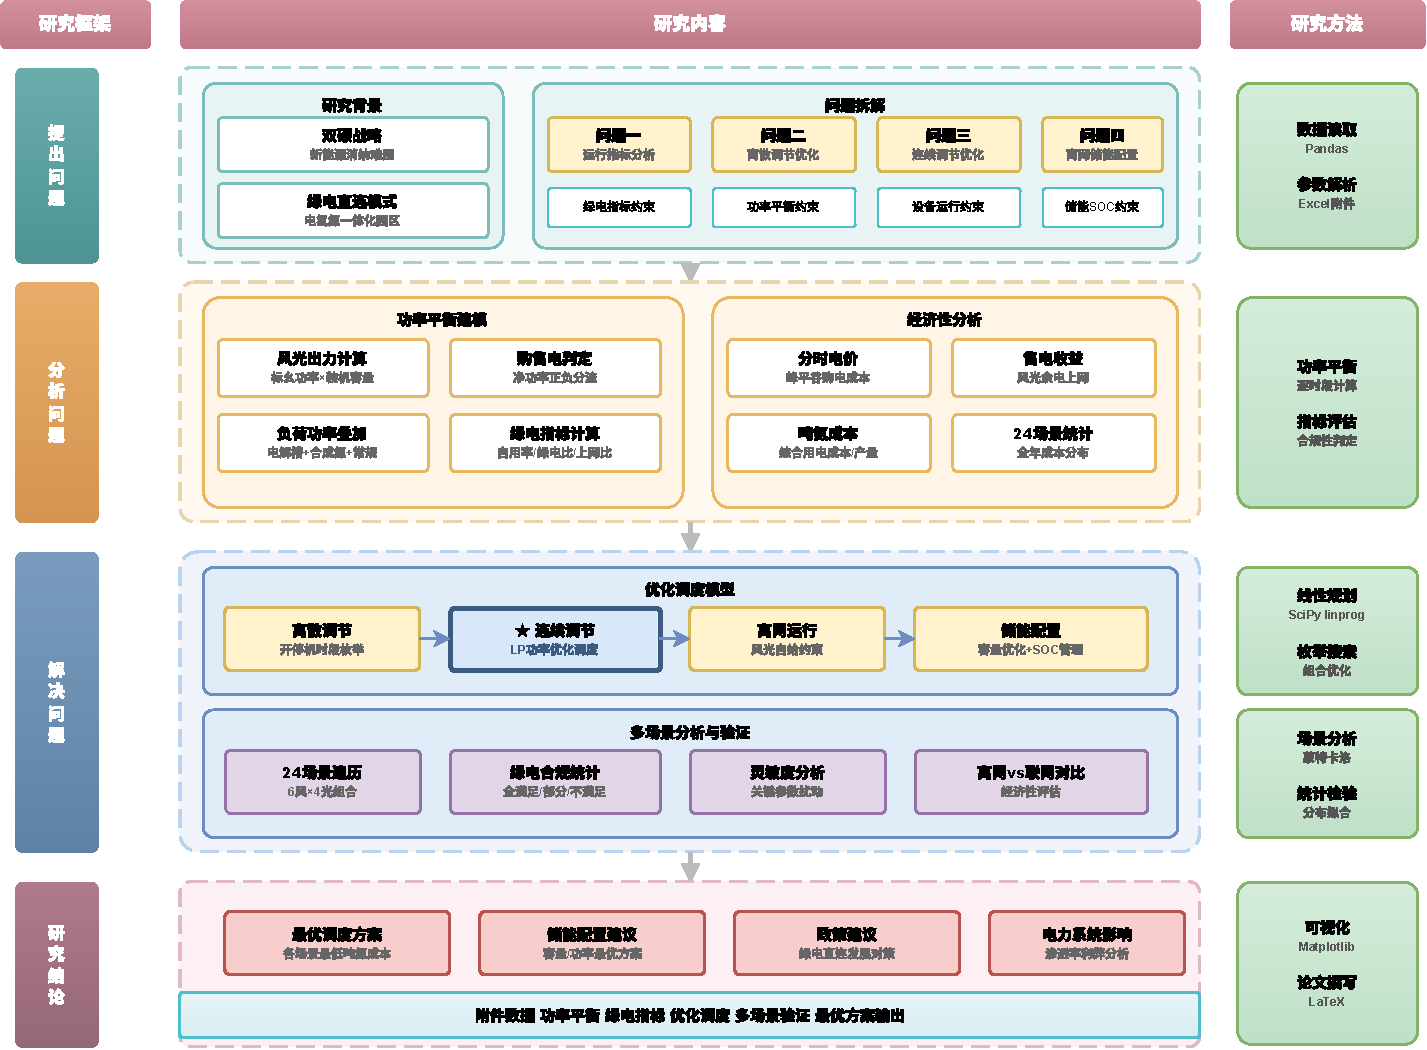
\includegraphics[width=\textwidth,height=0.45\textheight,keepaspectratio]{figures/fig_roadmap.pdf}
\caption{整体技术路线图}\label{fig:roadmap}
\end{figure}

% ==================== 园区系统架构图 ====================

\begin{figure}[H]
\centering
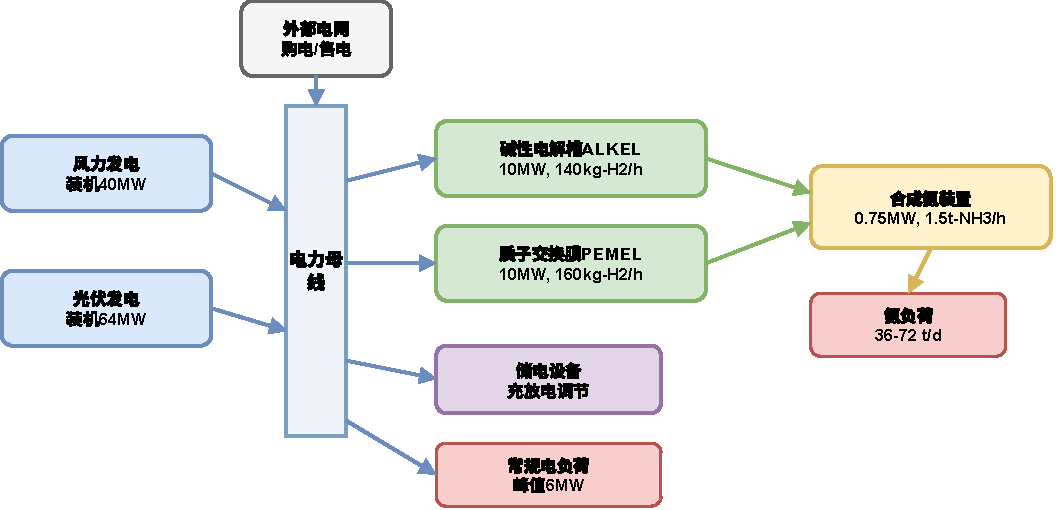
\includegraphics[width=0.9\textwidth,height=0.3\textheight,keepaspectratio]{figures/fig_system_arch.pdf}
\caption{绿电直连型电氢氨园区系统架构}\label{fig:system_arch}
\end{figure}

% ==================== 求解流程图 ====================

\begin{figure}[H]
\centering
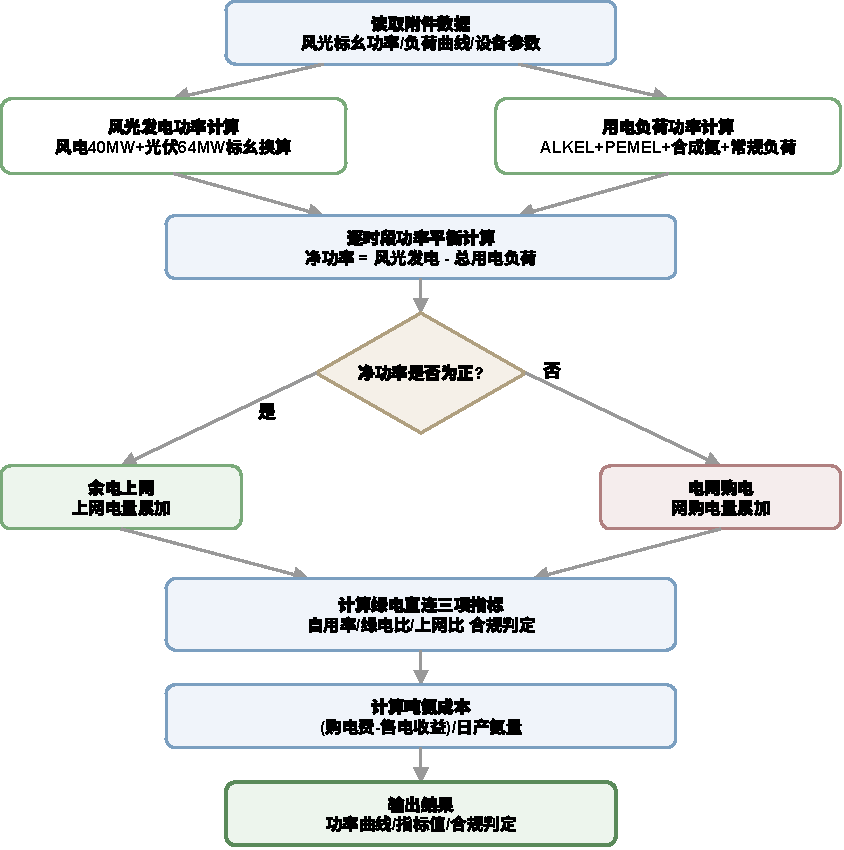
\includegraphics[width=0.85\textwidth,height=0.38\textheight,keepaspectratio]{figures/fig_flow_q1.pdf}
\caption{问题一求解流程图}\label{fig:flow_q1}
\end{figure}

\begin{figure}[H]
\centering
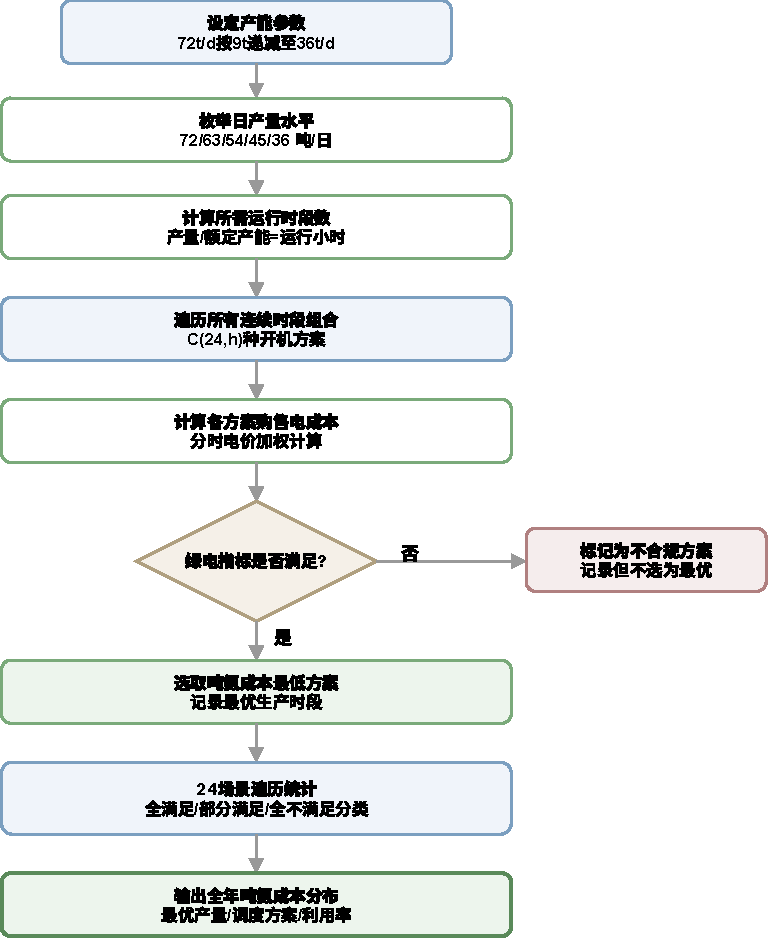
\includegraphics[width=0.85\textwidth,height=0.38\textheight,keepaspectratio]{figures/fig_flow_q2.pdf}
\caption{问题二求解流程图}\label{fig:flow_q2}
\end{figure}

\begin{figure}[H]
\centering
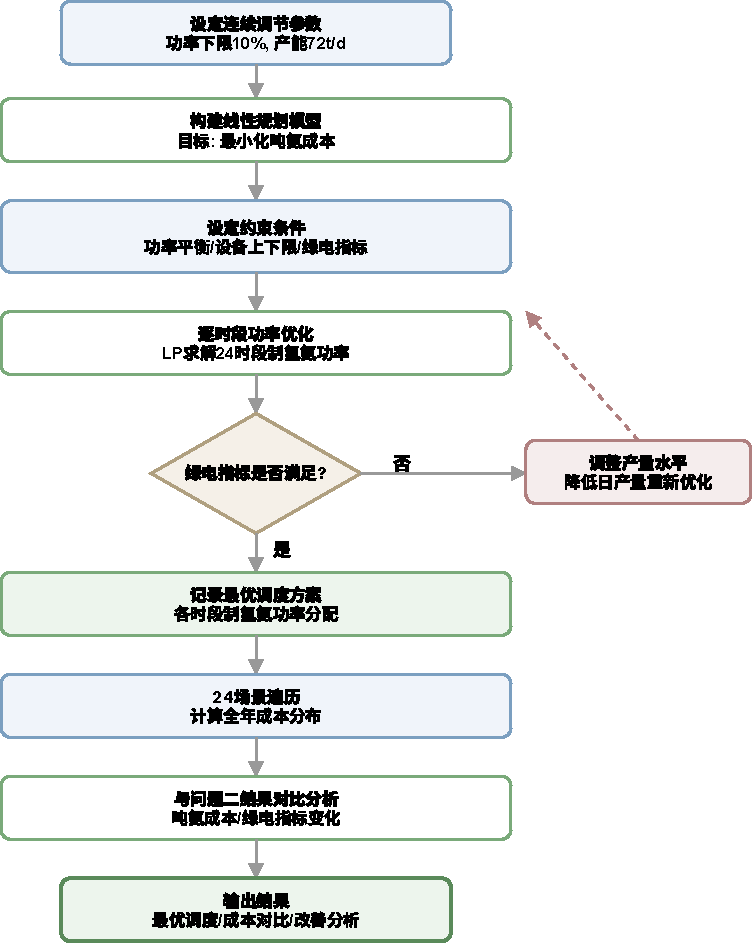
\includegraphics[width=0.85\textwidth,height=0.38\textheight,keepaspectratio]{figures/fig_flow_q3.pdf}
\caption{问题三求解流程图}\label{fig:flow_q3}
\end{figure}

\begin{figure}[H]
\centering
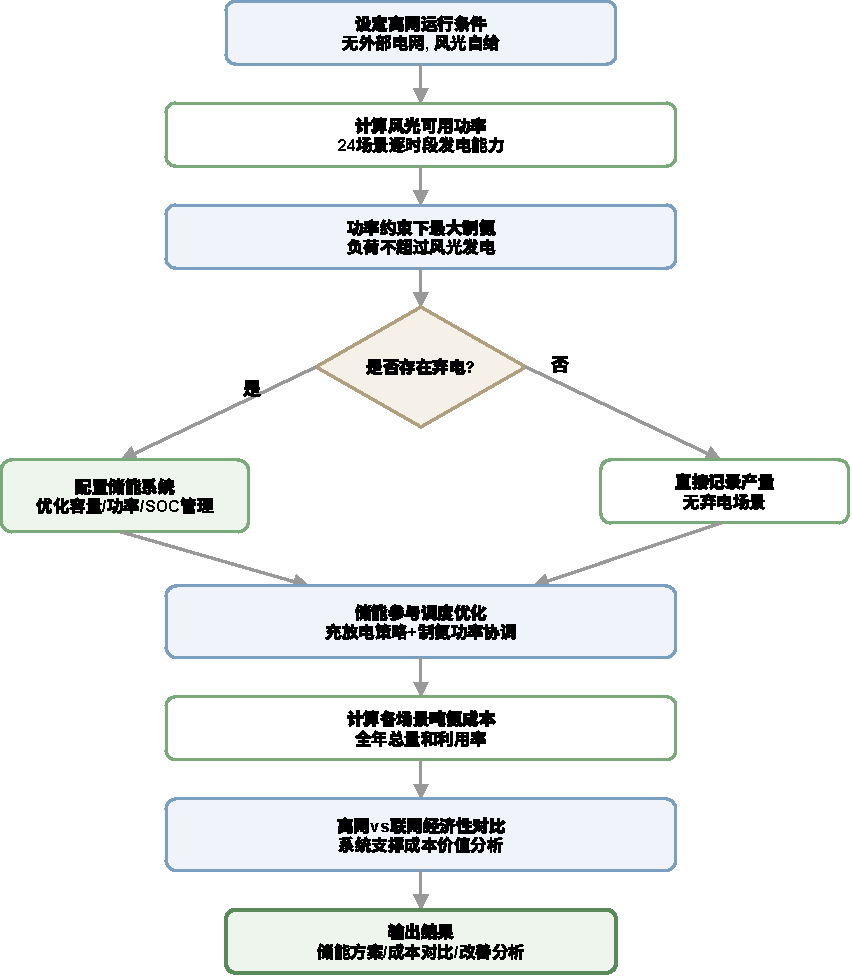
\includegraphics[width=0.85\textwidth,height=0.38\textheight,keepaspectratio]{figures/fig_flow_q4.pdf}
\caption{问题四求解流程图}\label{fig:flow_q4}
\end{figure}

% ==================== 问题一 ====================

\begin{figure}[H]
\centering
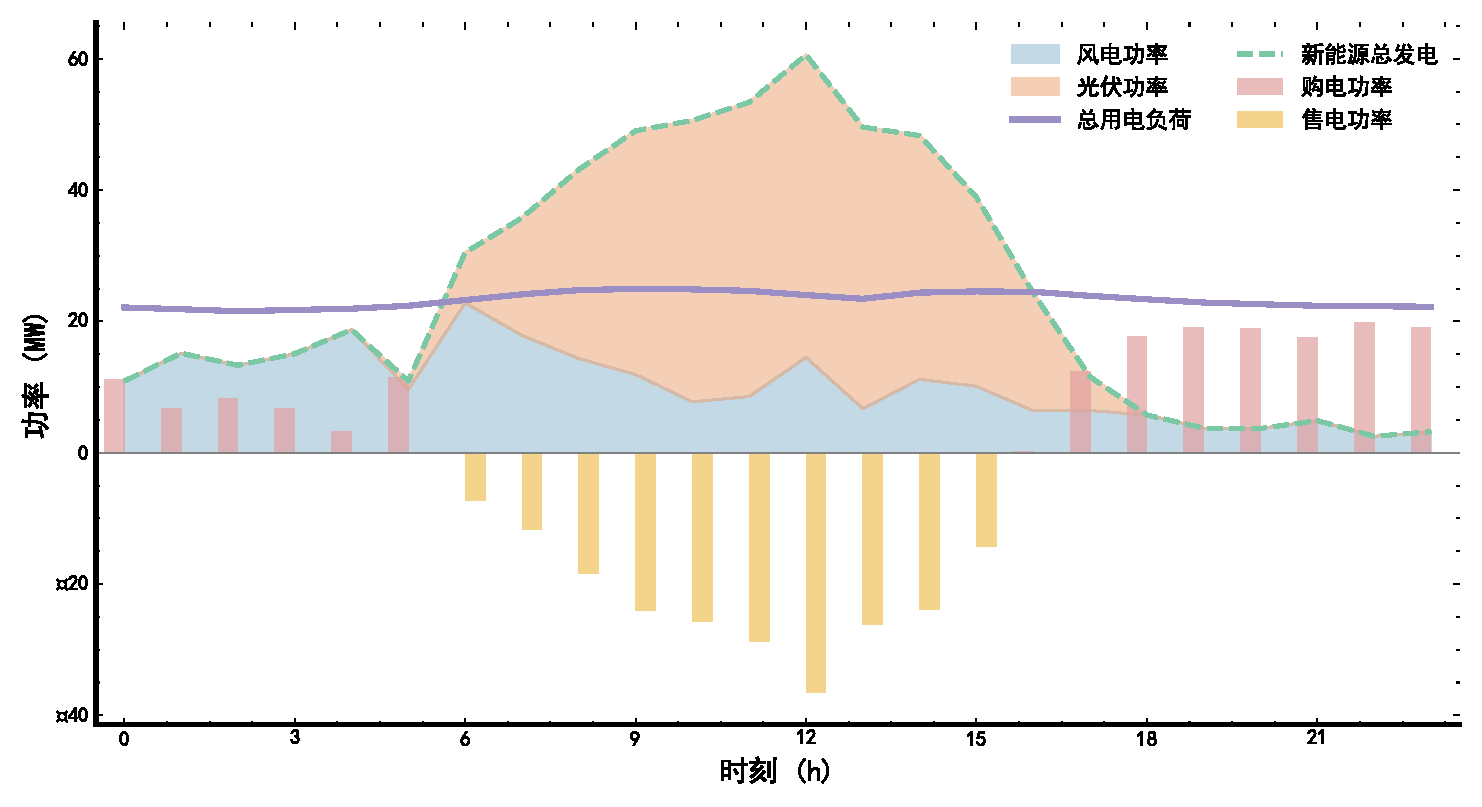
\includegraphics[width=0.95\textwidth]{figures/fig_q1_power_balance.pdf}
\caption{典型日功率平衡曲线（风电、光伏发电与负荷、购售电功率对比）}
\label{fig:q1_power_balance}
\end{figure}

\begin{figure}[H]
\centering
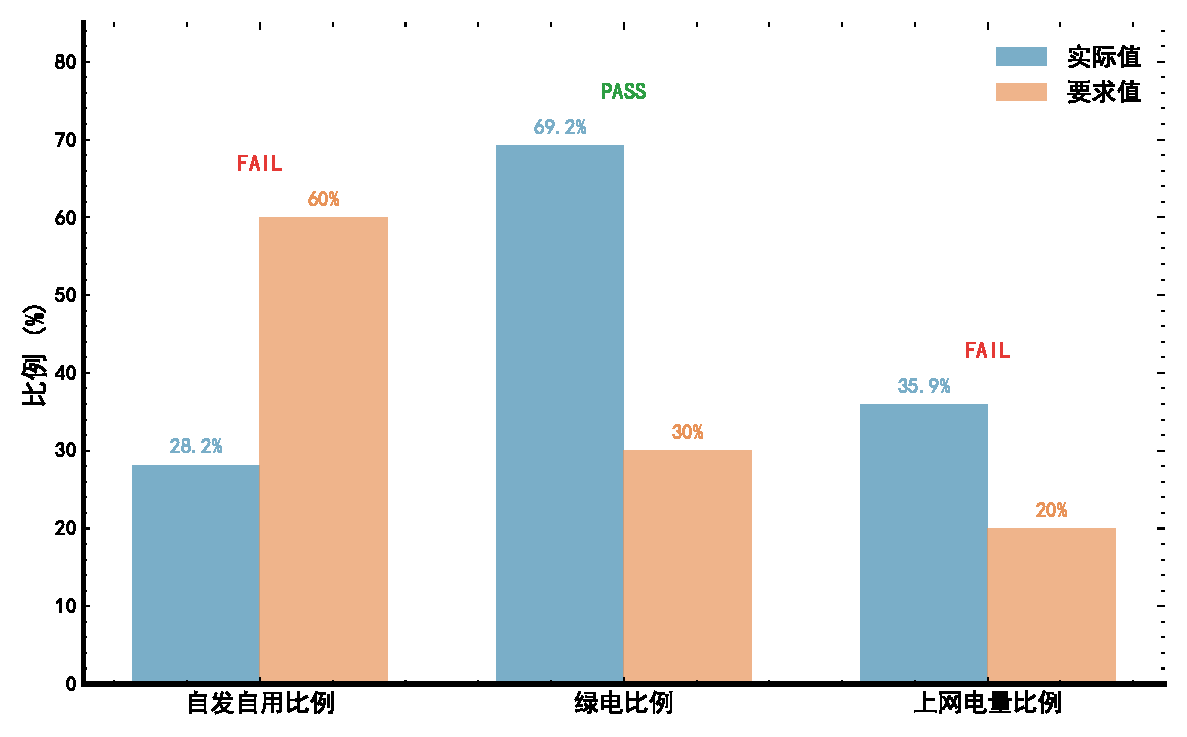
\includegraphics[width=0.75\textwidth]{figures/fig_q1_indicators.pdf}
\caption{绿电直连指标实际值与要求值对比}
\label{fig:q1_indicators}
\end{figure}

% ==================== 问题二 ====================

\begin{figure}[H]
\centering
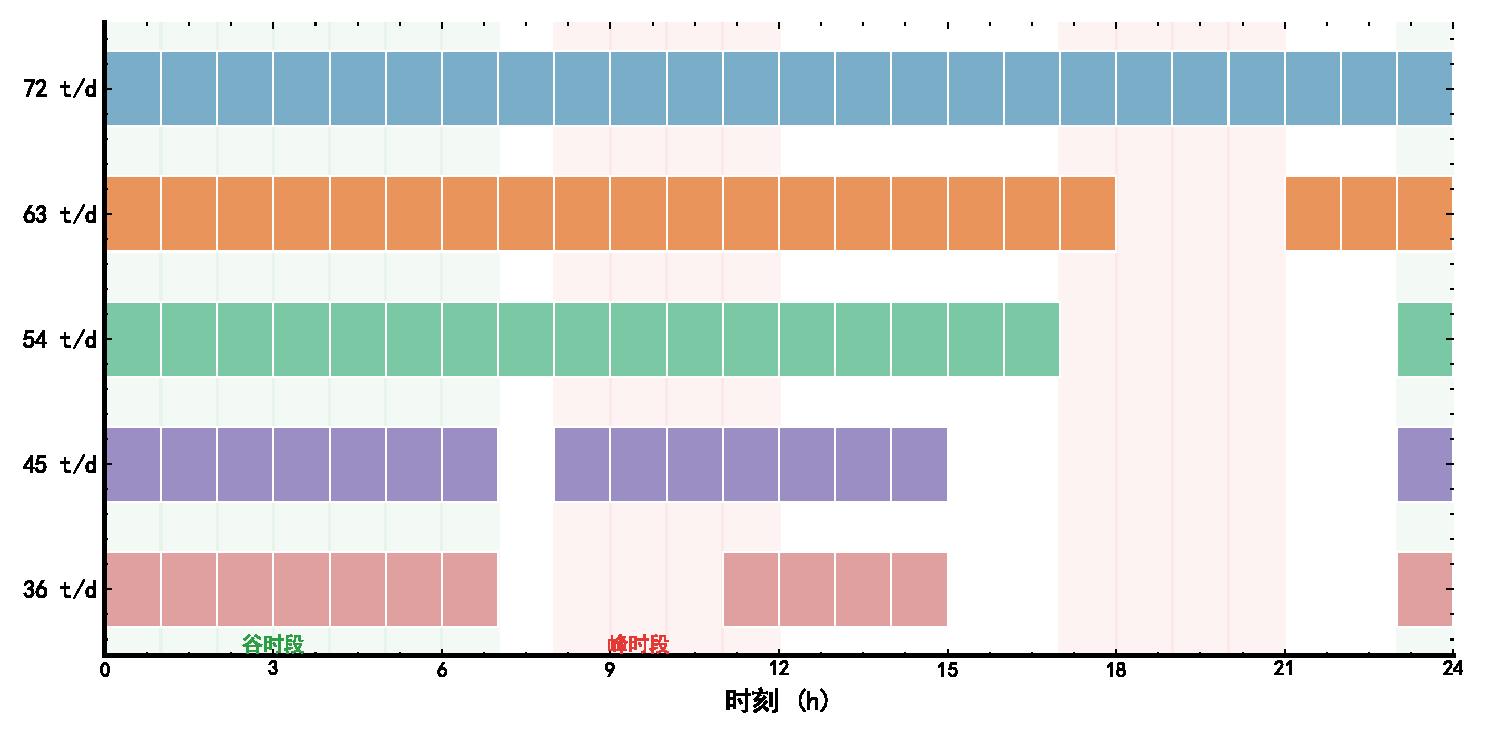
\includegraphics[width=0.92\textwidth]{figures/fig_q2_gantt.pdf}
\caption{不同产量下最优开机时段安排甘特图}
\label{fig:q2_gantt}
\end{figure}

\begin{figure}[H]
\centering
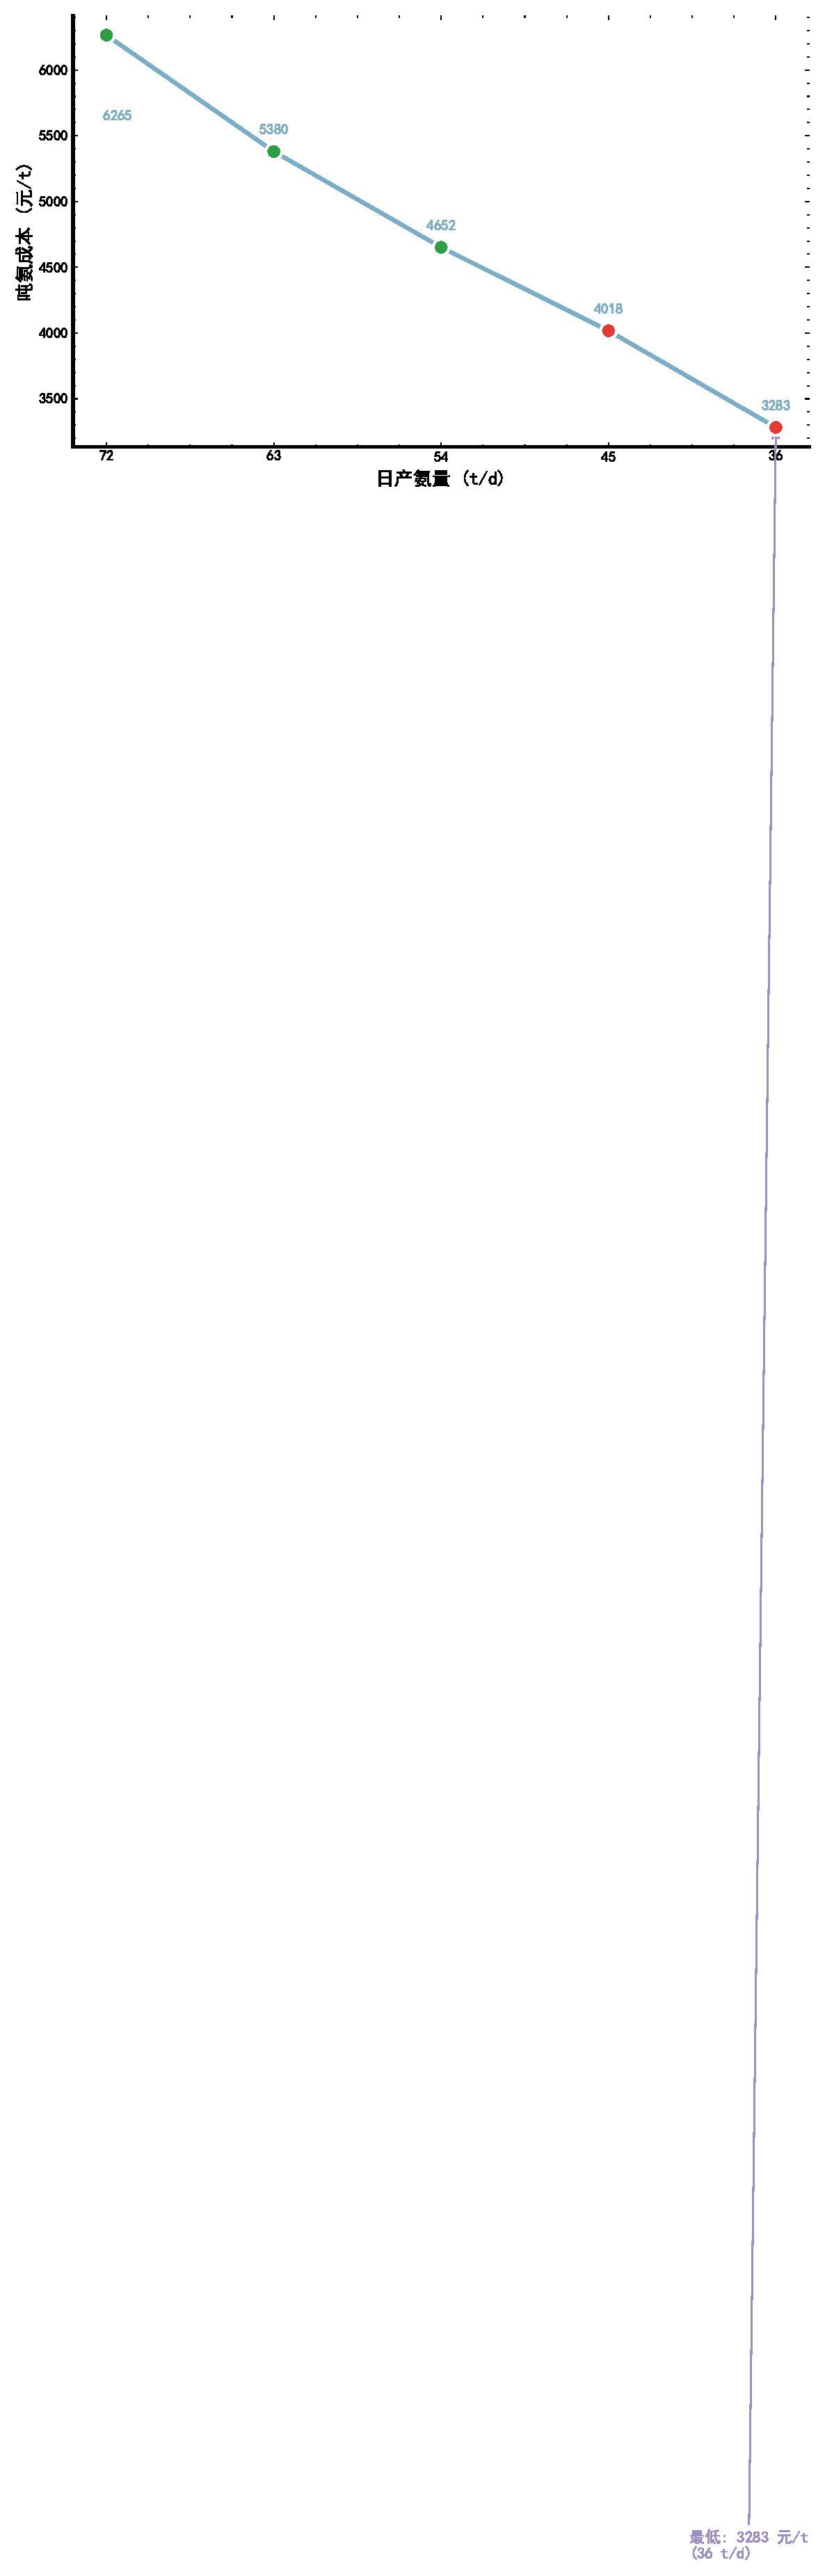
\includegraphics[width=0.78\textwidth]{figures/fig_q2_cost_vs_production.pdf}
\caption{吨氨成本随日产量变化曲线}
\label{fig:q2_cost_vs_production}
\end{figure}

\begin{figure}[H]
\centering
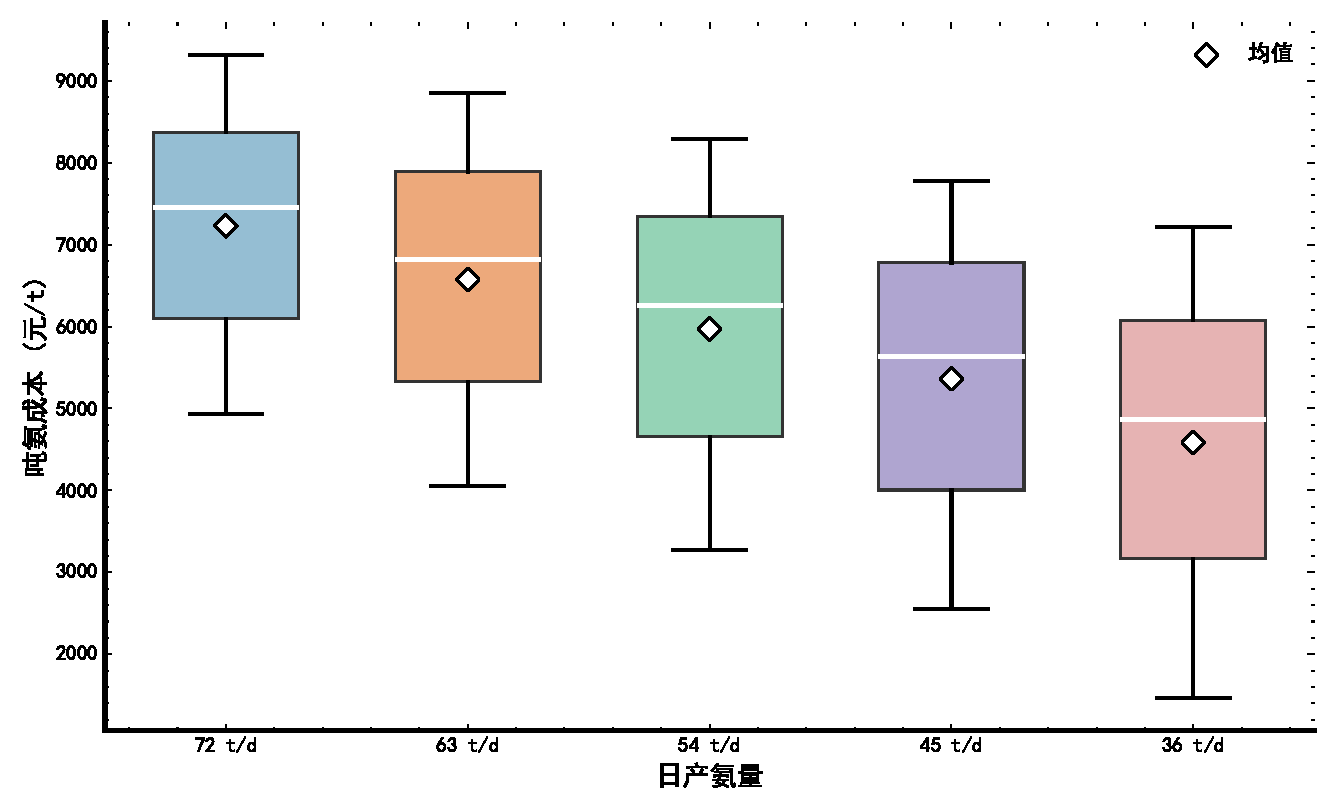
\includegraphics[width=0.82\textwidth]{figures/fig_q2_24scenes_cost.pdf}
\caption{24种风光场景下各产量吨氨成本分布箱线图}
\label{fig:q2_24scenes_cost}
\end{figure}

\begin{figure}[H]
\centering
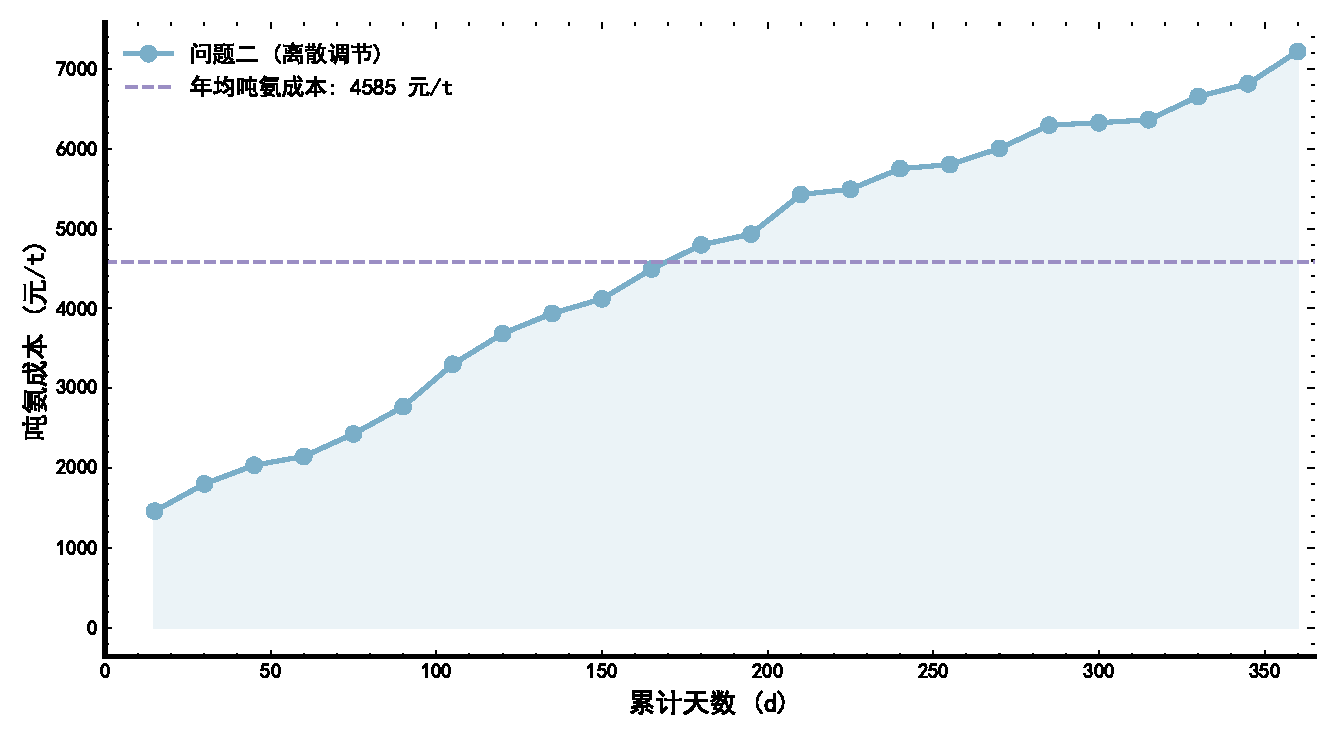
\includegraphics[width=0.85\textwidth]{figures/fig_q2_annual_cost.pdf}
\caption{全年吨氨成本分布曲线（问题二，离散调节，36 t/d）}
\label{fig:q2_annual_cost}
\end{figure}

\begin{figure}[H]
\centering
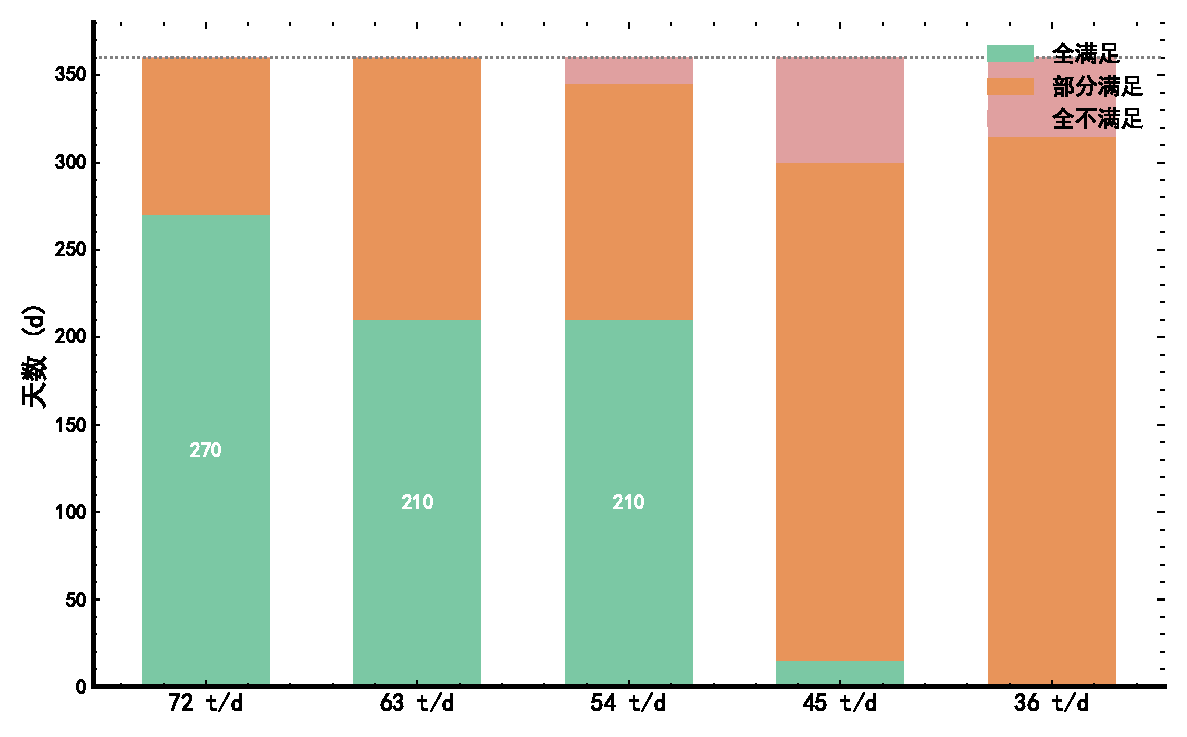
\includegraphics[width=0.78\textwidth]{figures/fig_q2_indicator_stats.pdf}
\caption{全年绿电直连指标满足情况统计}
\label{fig:q2_indicator_stats}
\end{figure}

% ==================== 问题三 ====================

\begin{figure}[H]
\centering
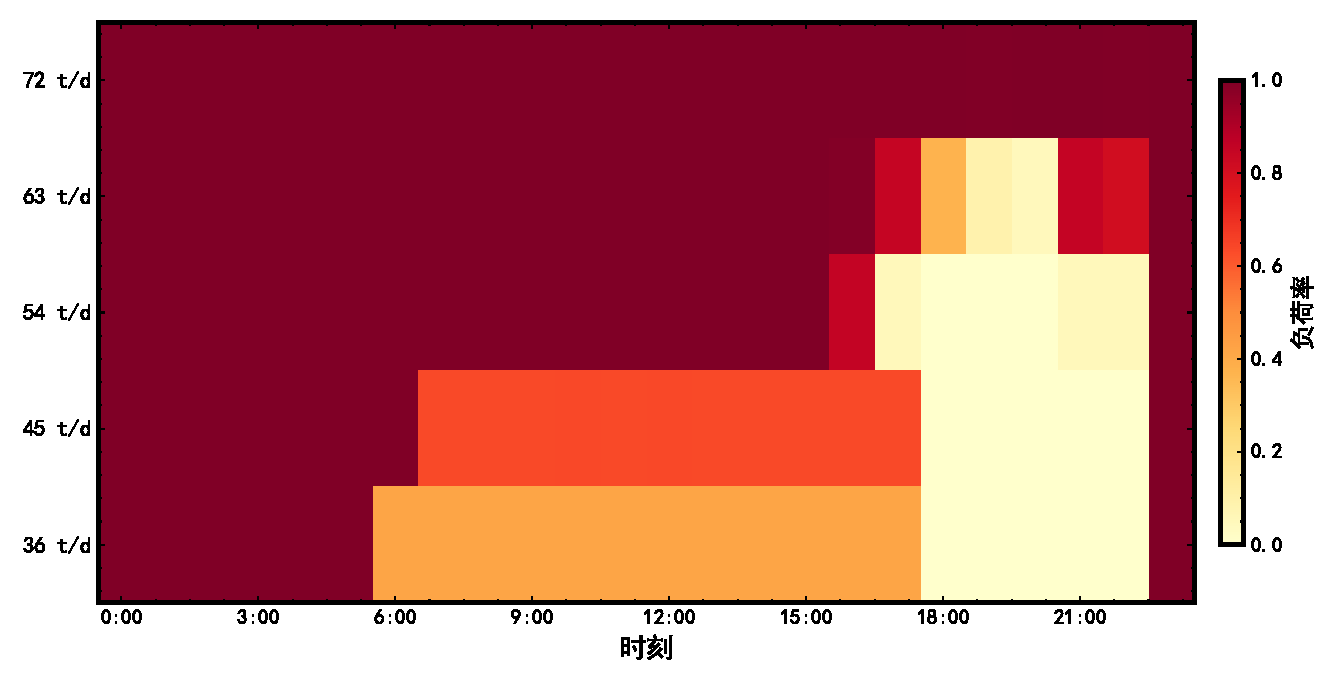
\includegraphics[width=0.92\textwidth]{figures/fig_q3_dispatch.pdf}
\caption{连续调节模式下各产量典型场景负荷率调度热力图}
\label{fig:q3_dispatch}
\end{figure}

\begin{figure}[H]
\centering
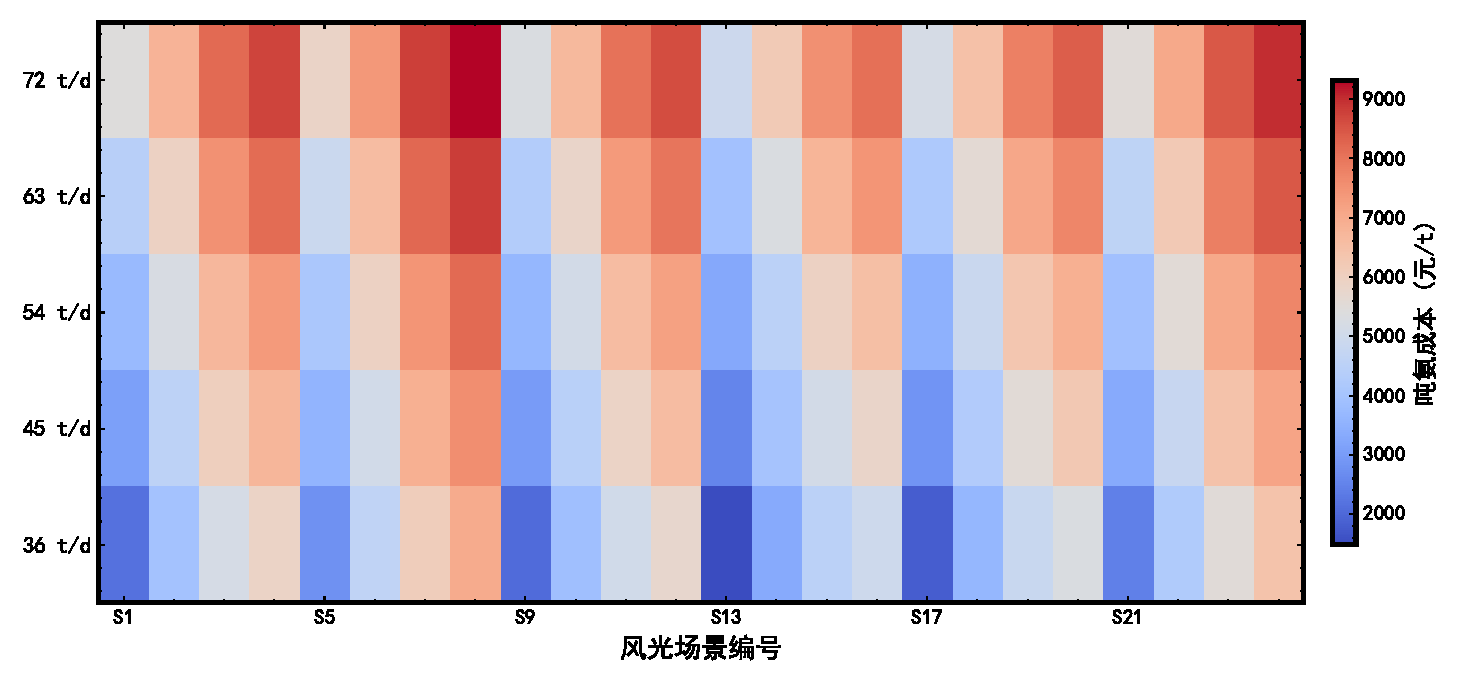
\includegraphics[width=0.92\textwidth]{figures/fig_q3_alpha_heatmap.pdf}
\caption{24种场景下各产量吨氨成本热力图}
\label{fig:q3_alpha_heatmap}
\end{figure}

\begin{figure}[H]
\centering
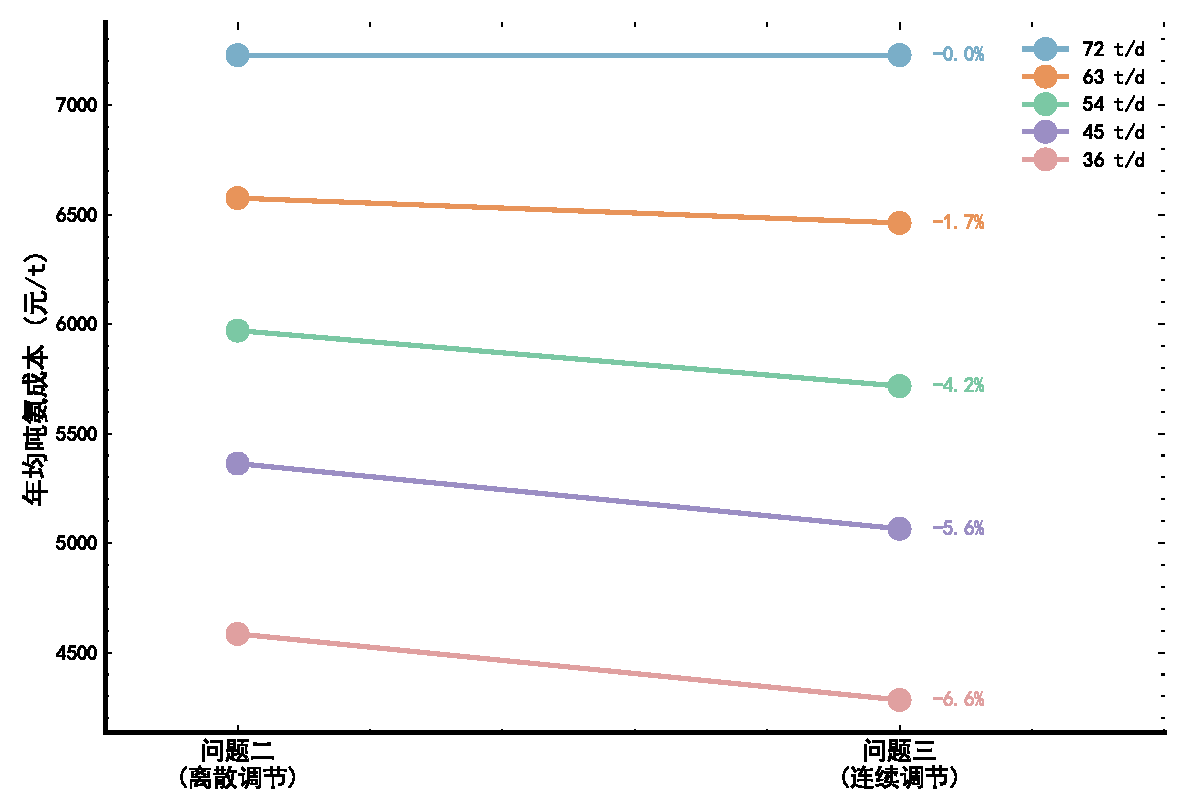
\includegraphics[width=0.78\textwidth]{figures/fig_q3_compare_q2.pdf}
\caption{问题三与问题二年均吨氨成本配对对比图}
\label{fig:q3_compare_q2}
\end{figure}

\begin{figure}[H]
\centering
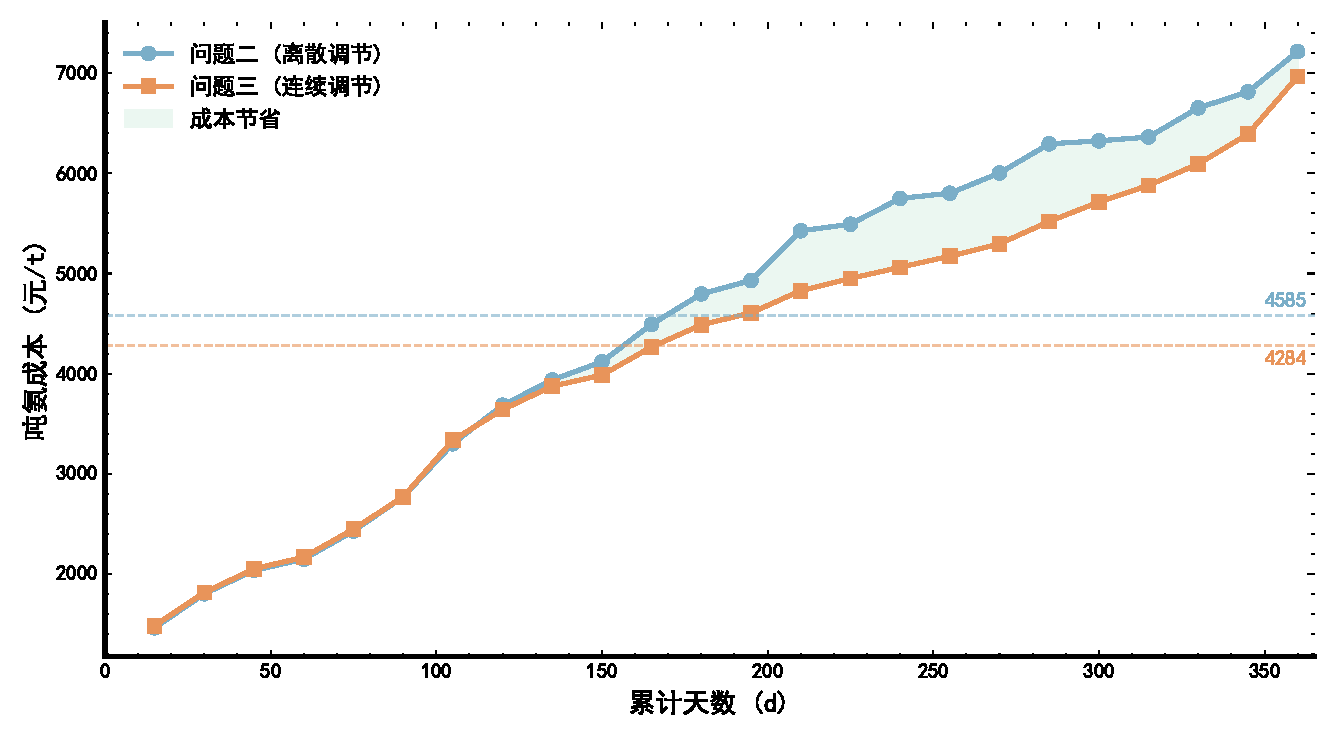
\includegraphics[width=0.85\textwidth]{figures/fig_q3_annual_cost.pdf}
\caption{全年吨氨成本分布曲线（问题二与问题三对比）}
\label{fig:q3_annual_cost}
\end{figure}

% ==================== 问题四 ====================

\begin{figure}[H]
\centering
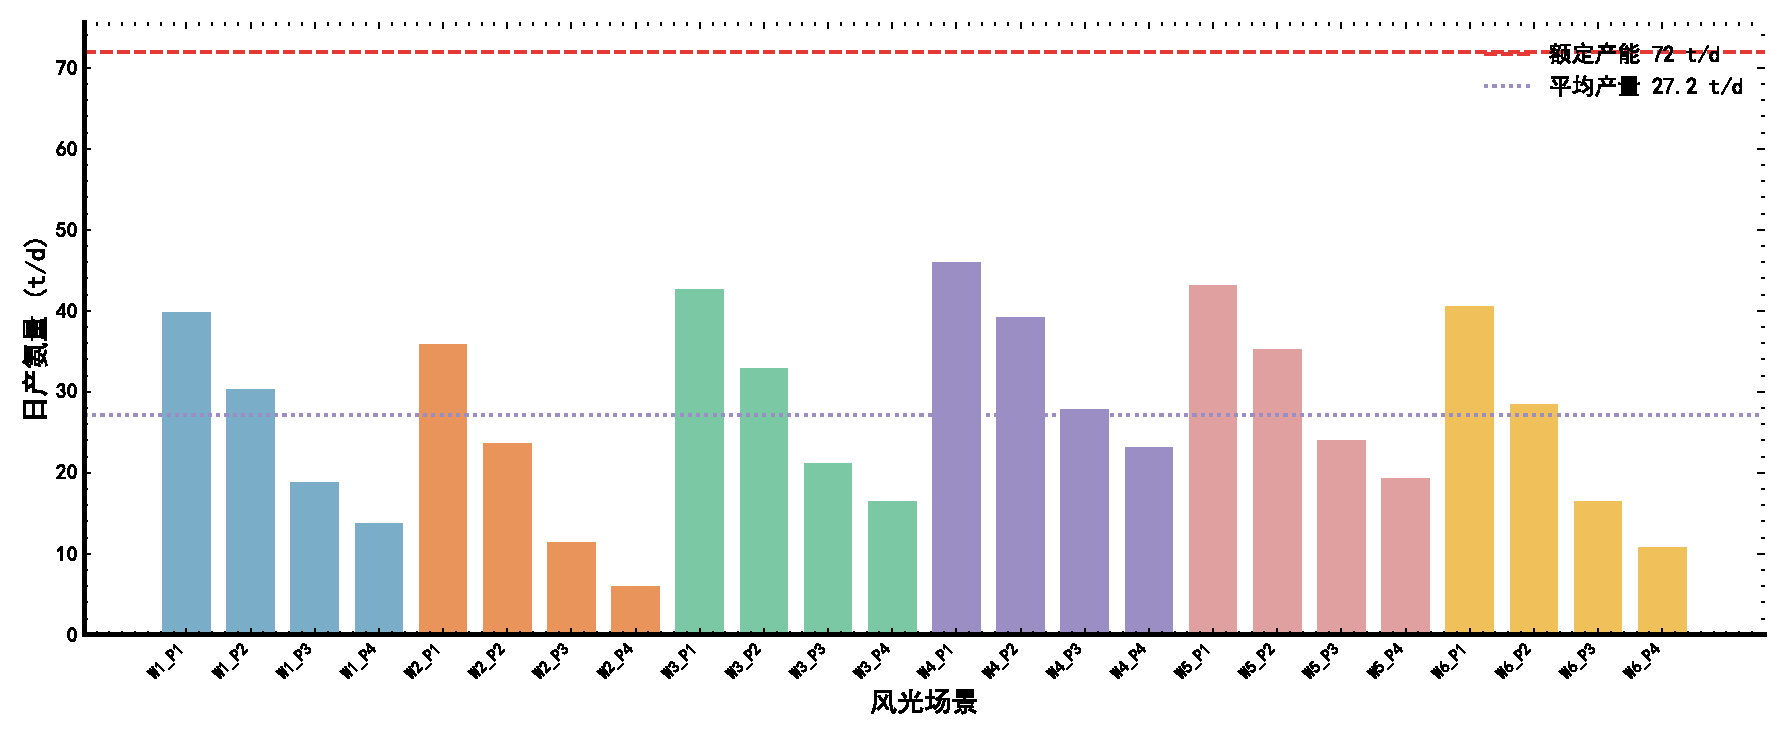
\includegraphics[width=0.95\textwidth]{figures/fig_q4_offgrid_production.pdf}
\caption{24种风光场景下离网运行日产氨量}
\label{fig:q4_offgrid_production}
\end{figure}

\begin{figure}[H]
\centering
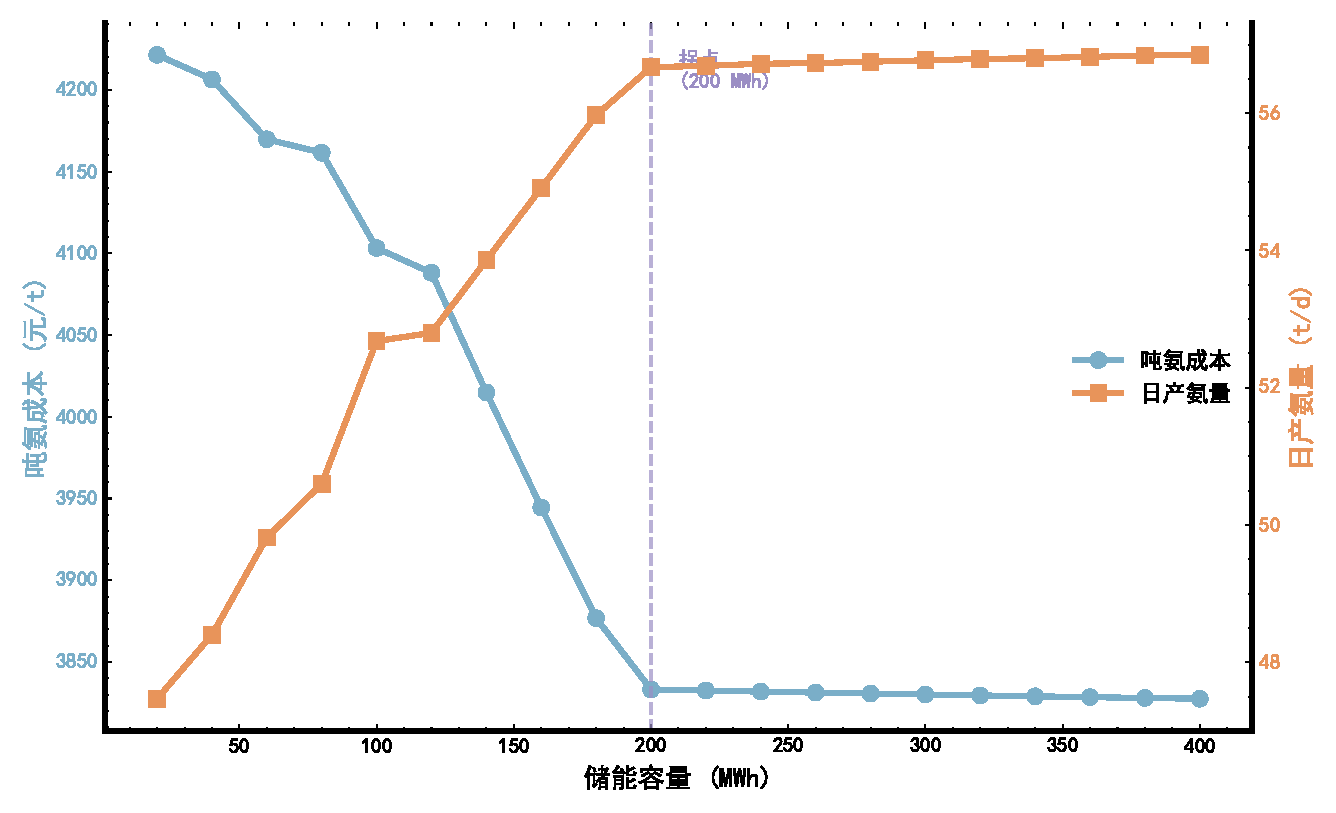
\includegraphics[width=0.82\textwidth]{figures/fig_q4_storage_optimization.pdf}
\caption{储能容量与吨氨成本、日产氨量关系曲线}
\label{fig:q4_storage_optimization}
\end{figure}

\begin{figure}[H]
\centering
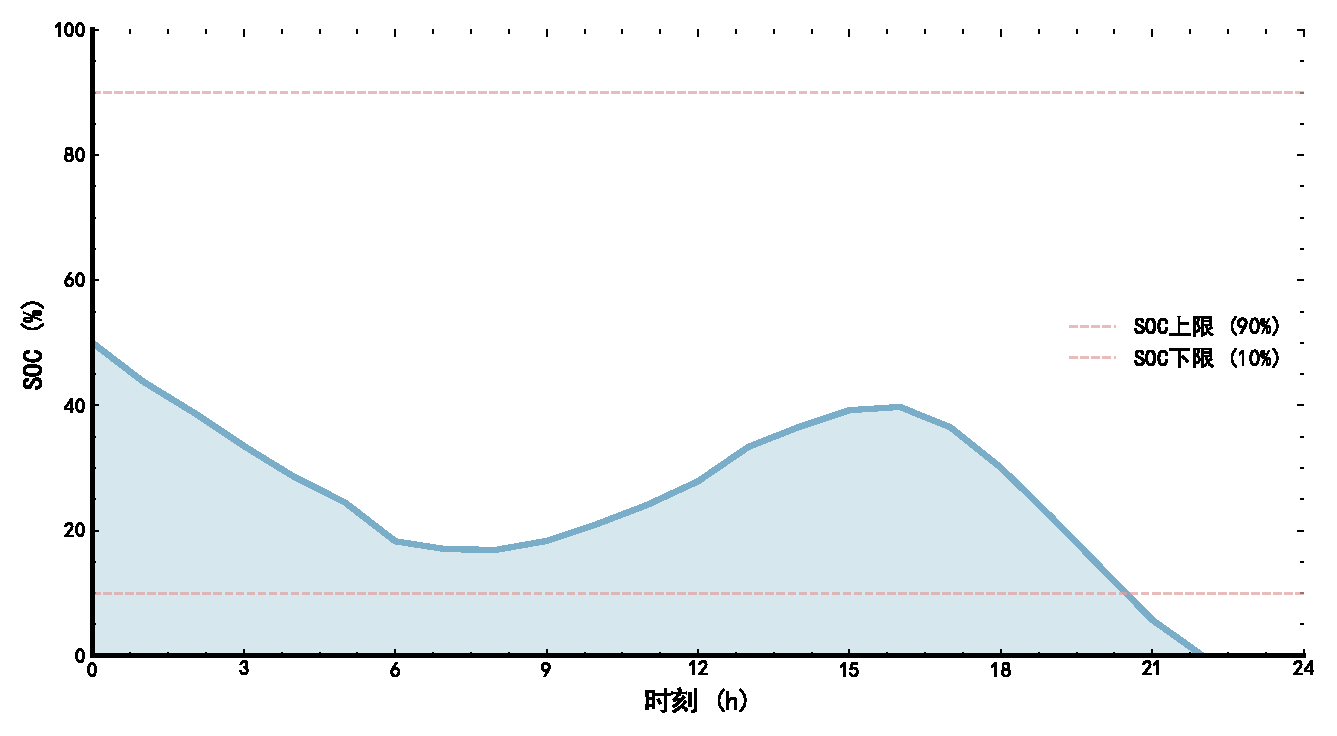
\includegraphics[width=0.82\textwidth]{figures/fig_q4_soc_curve.pdf}
\caption{最大弃电场景储能SOC变化曲线}
\label{fig:q4_soc_curve}
\end{figure}

\begin{figure}[H]
\centering
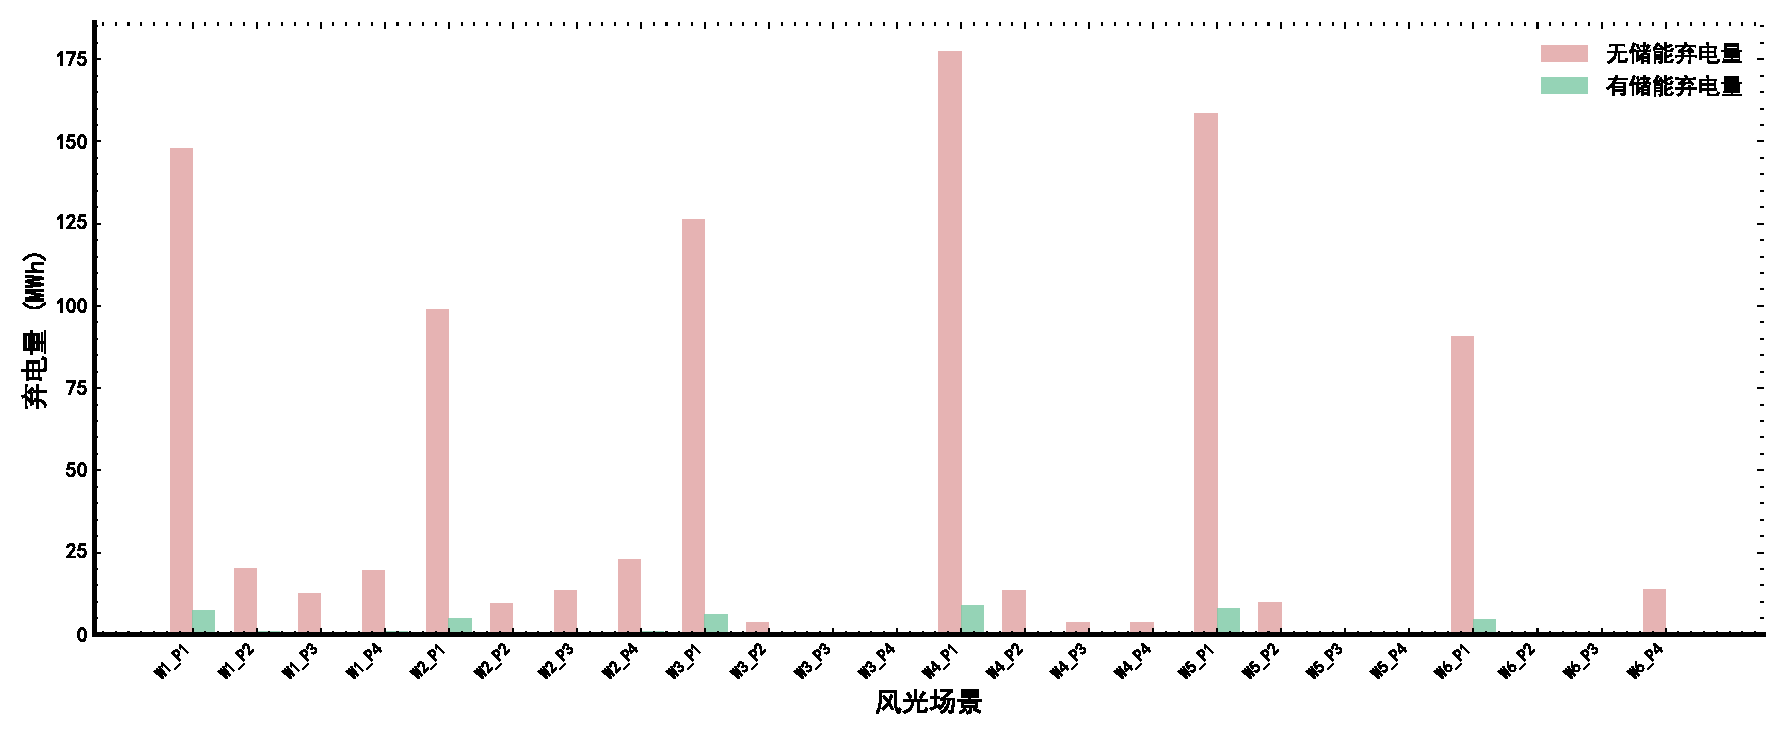
\includegraphics[width=0.95\textwidth]{figures/fig_q4_curtail_compare.pdf}
\caption{有无储能弃电量对比}
\label{fig:q4_curtail_compare}
\end{figure}

\begin{figure}[H]
\centering
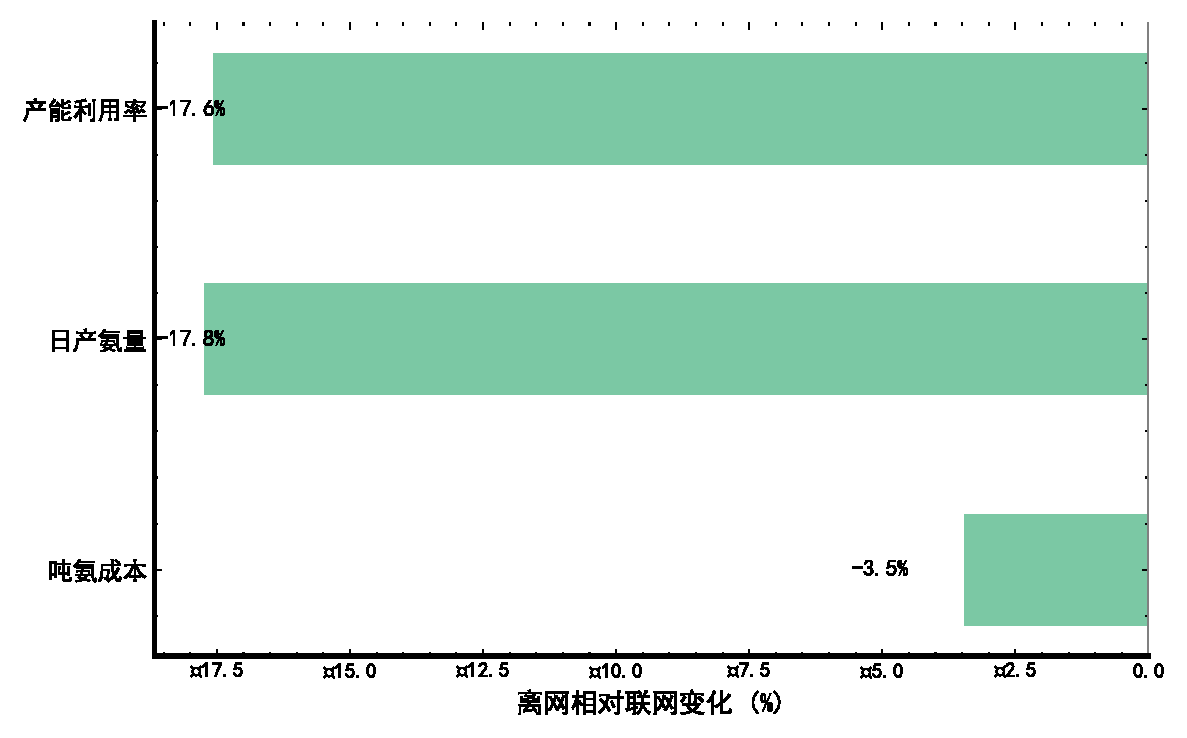
\includegraphics[width=0.75\textwidth]{figures/fig_q4_onoff_compare.pdf}
\caption{离网与联网运行模式经济性对比（发散柱状图）}
\label{fig:q4_onoff_compare}
\end{figure}

% ==================== 灵敏度分析 ====================

\begin{figure}[H]
\centering
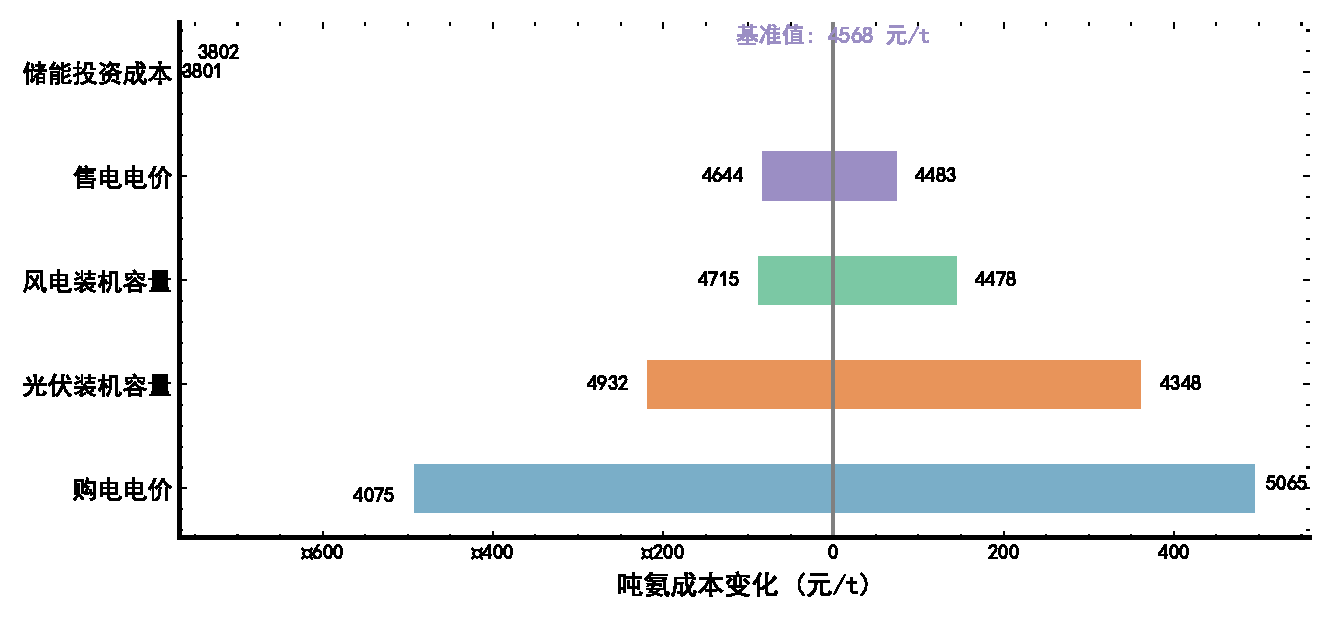
\includegraphics[width=0.82\textwidth]{figures/fig_sensitivity.pdf}
\caption{关键参数敏感性分析龙卷风图}
\label{fig:sensitivity}
\end{figure}

% ============================================================

% ==================== 技术路线图 ====================

\begin{figure}[H]
\centering
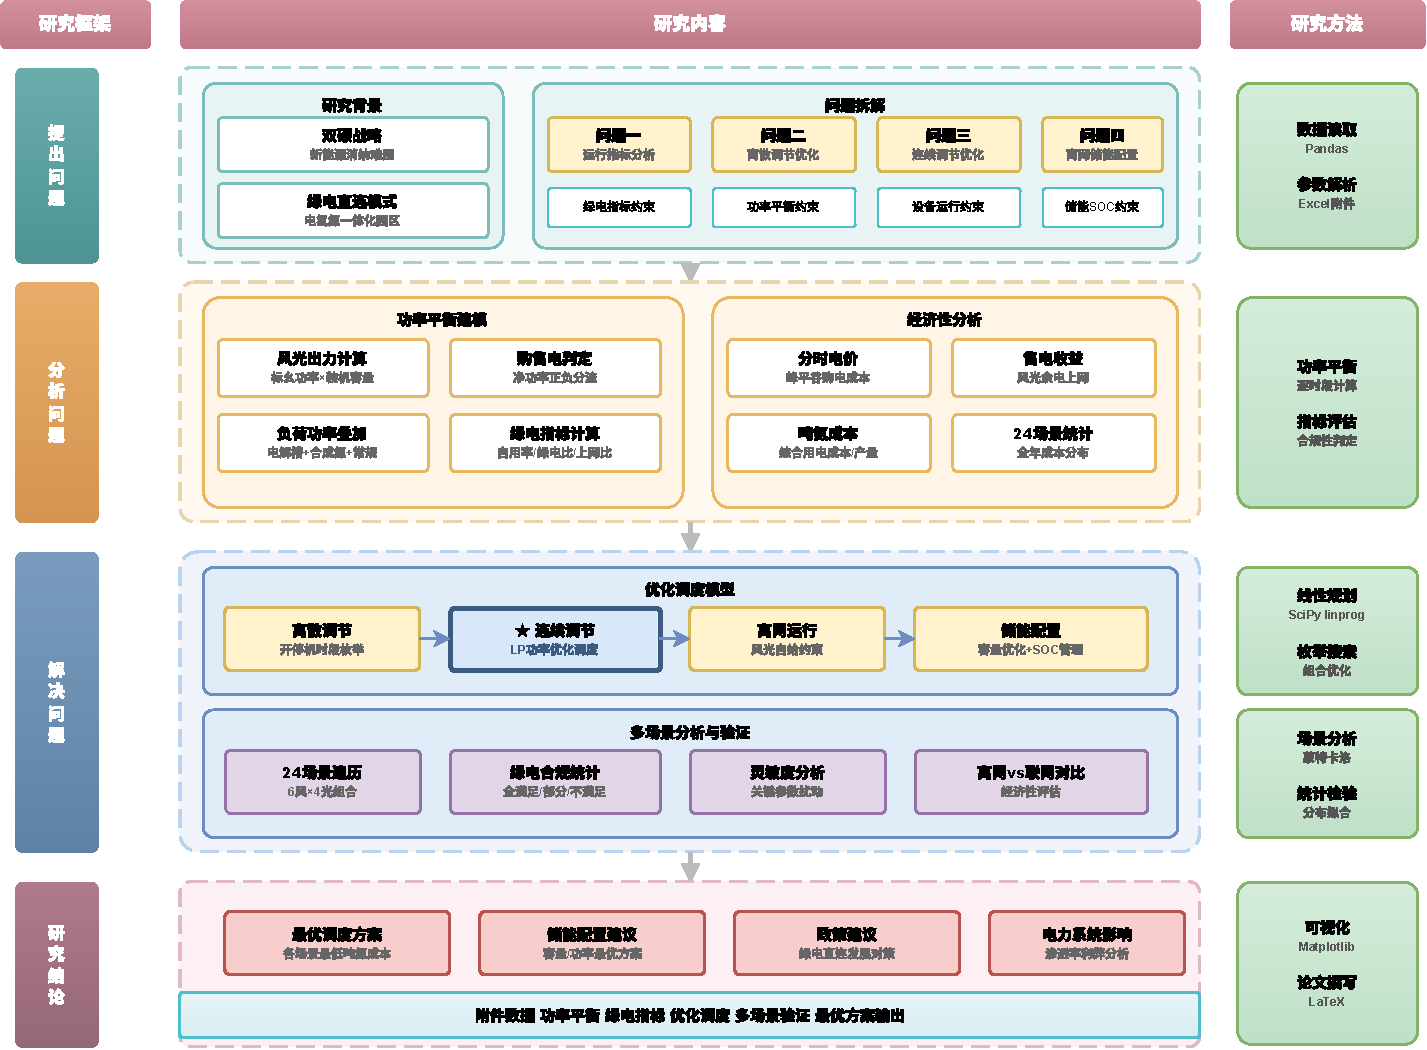
\includegraphics[width=\textwidth,height=0.45\textheight,keepaspectratio]{figures/fig_roadmap.pdf}
\caption{整体技术路线图}\label{fig:roadmap}
\end{figure}

% ==================== 园区系统架构图 ====================

\begin{figure}[H]
\centering
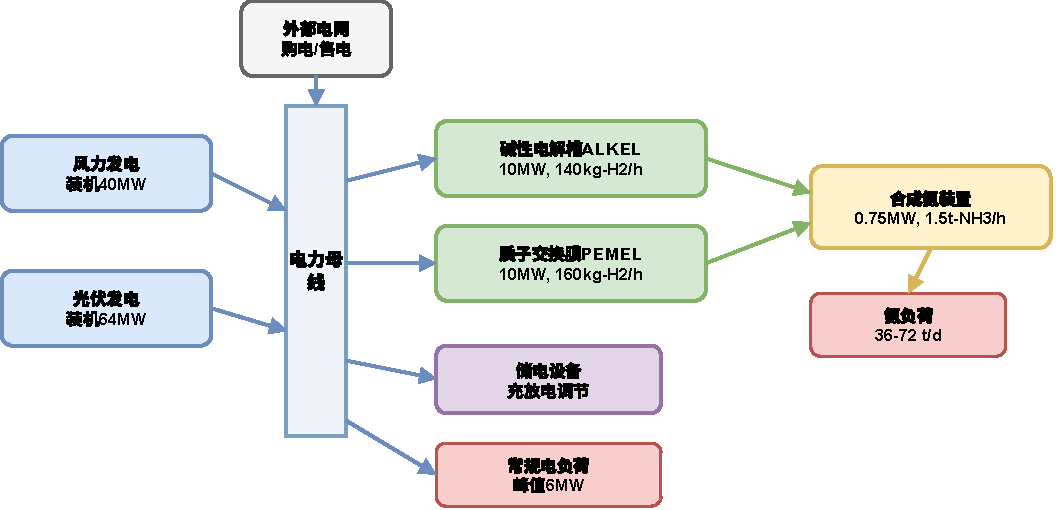
\includegraphics[width=0.9\textwidth,height=0.3\textheight,keepaspectratio]{figures/fig_system_arch.pdf}
\caption{绿电直连型电氢氨园区系统架构}\label{fig:system_arch}
\end{figure}

% ==================== 求解流程图 ====================

\begin{figure}[H]
\centering
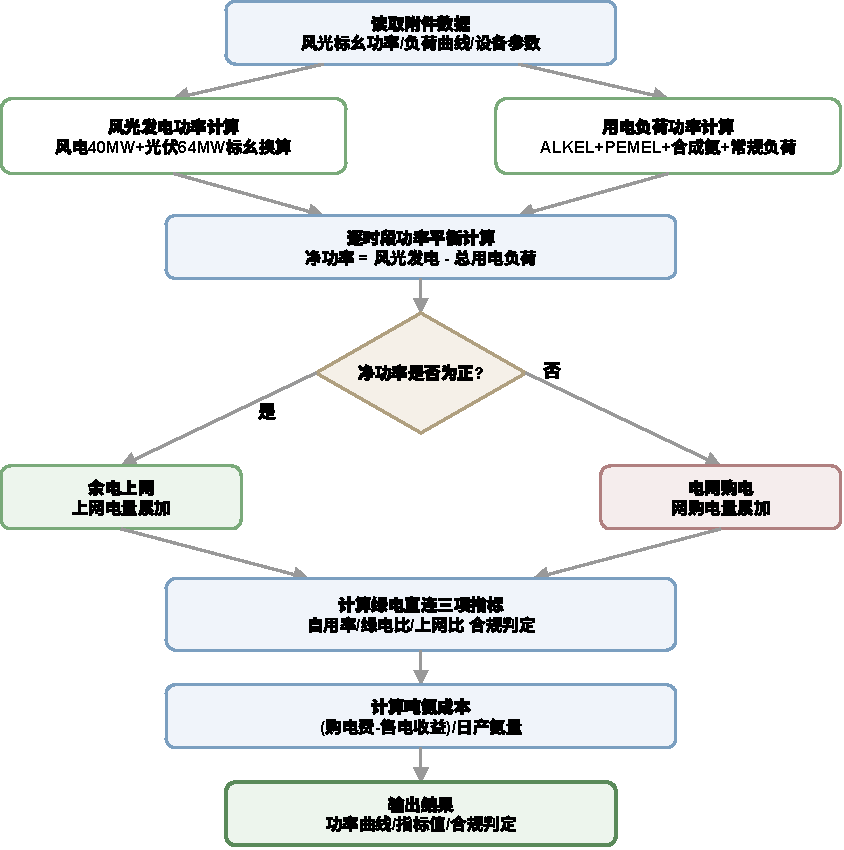
\includegraphics[width=0.85\textwidth,height=0.38\textheight,keepaspectratio]{figures/fig_flow_q1.pdf}
\caption{问题一求解流程图}\label{fig:flow_q1}
\end{figure}

\begin{figure}[H]
\centering
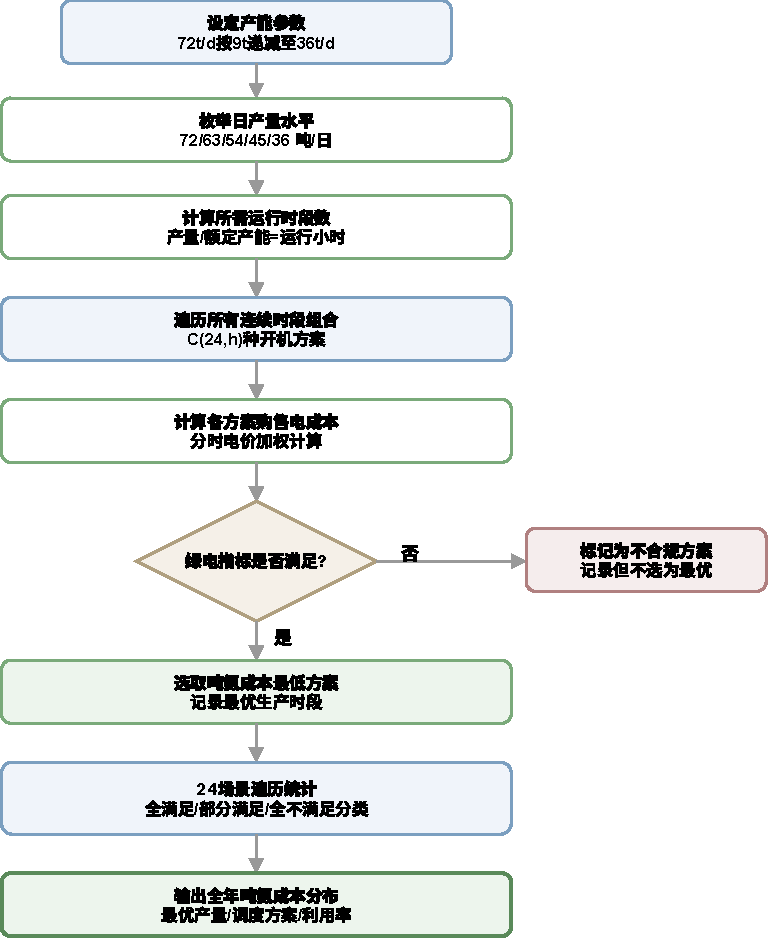
\includegraphics[width=0.85\textwidth,height=0.38\textheight,keepaspectratio]{figures/fig_flow_q2.pdf}
\caption{问题二求解流程图}\label{fig:flow_q2}
\end{figure}

\begin{figure}[H]
\centering
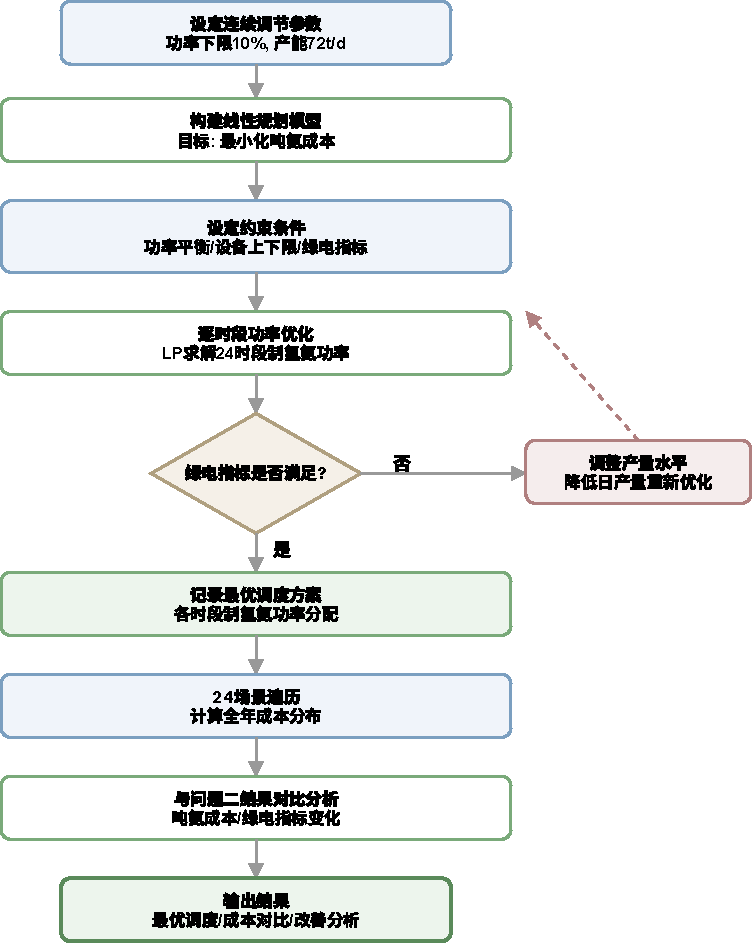
\includegraphics[width=0.85\textwidth,height=0.38\textheight,keepaspectratio]{figures/fig_flow_q3.pdf}
\caption{问题三求解流程图}\label{fig:flow_q3}
\end{figure}

\begin{figure}[H]
\centering
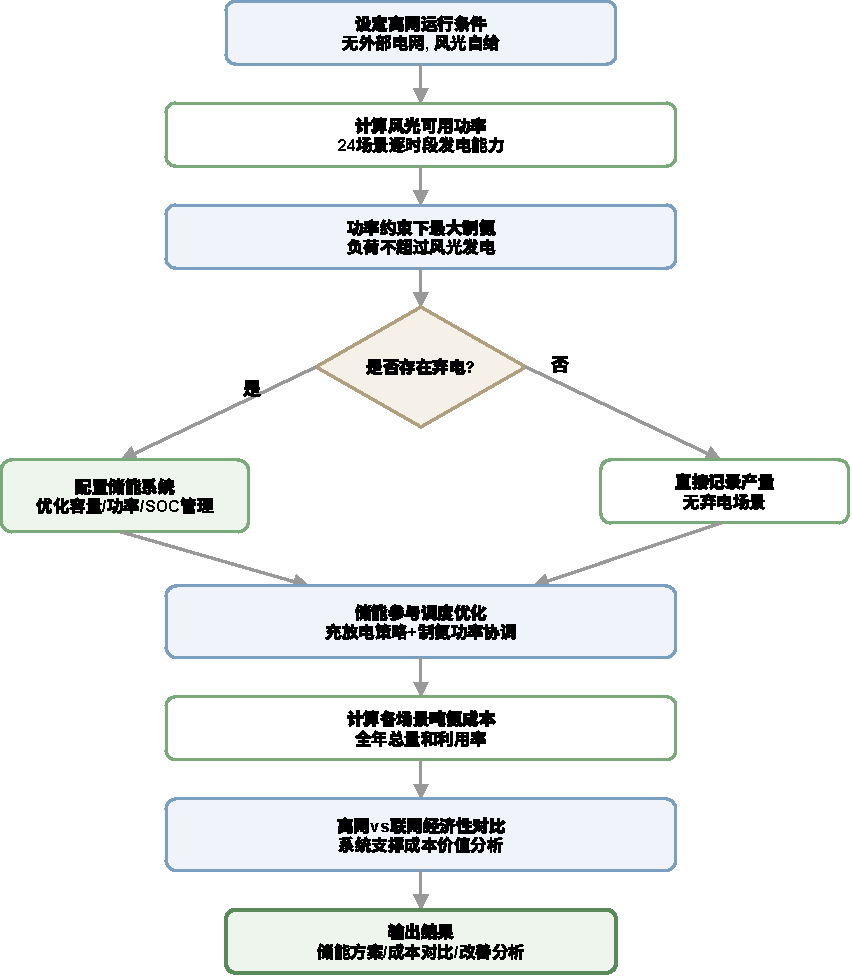
\includegraphics[width=0.85\textwidth,height=0.38\textheight,keepaspectratio]{figures/fig_flow_q4.pdf}
\caption{问题四求解流程图}\label{fig:flow_q4}
\end{figure}

% ==================== 问题一 ====================

\begin{figure}[H]
\centering
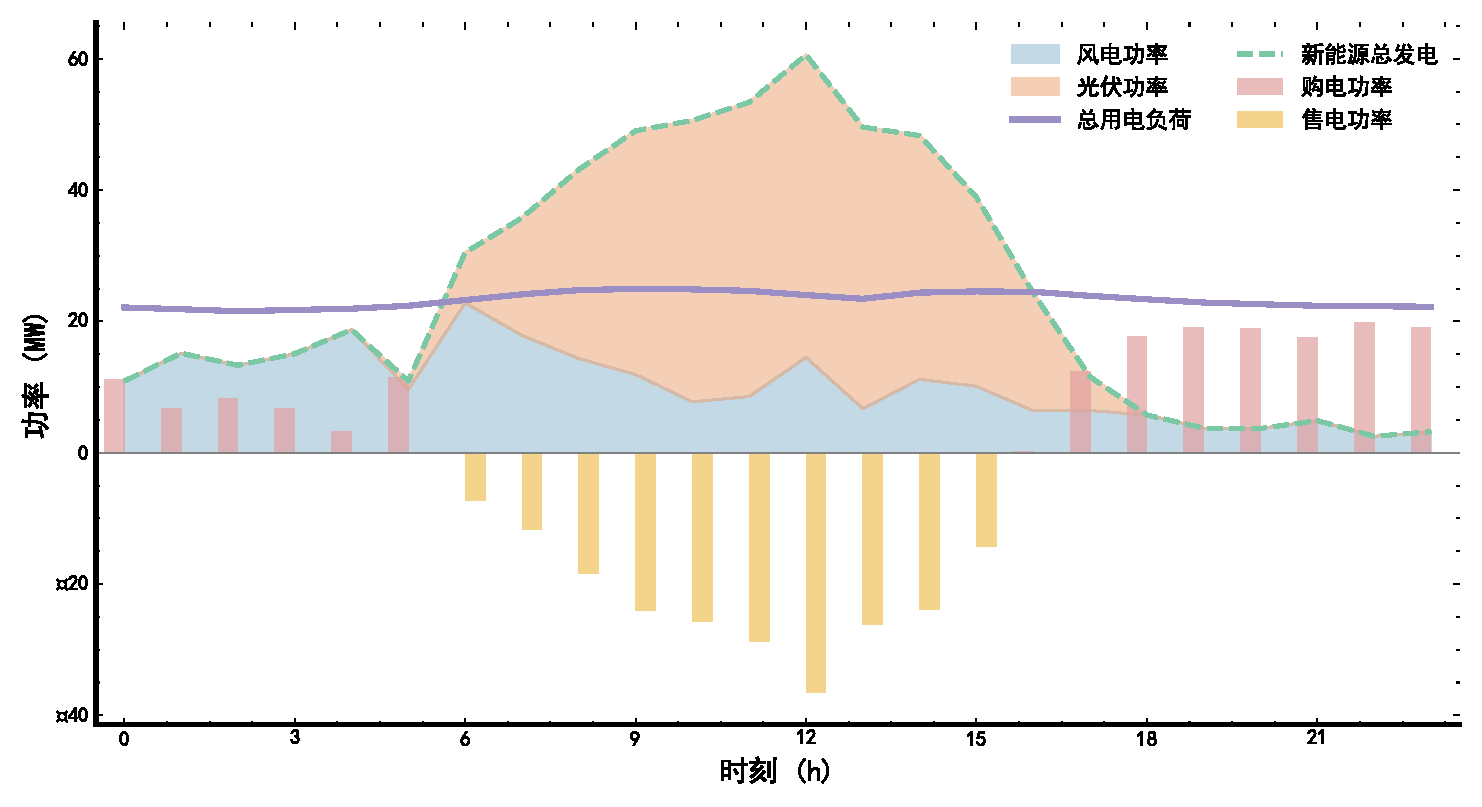
\includegraphics[width=0.95\textwidth]{figures/fig_q1_power_balance.pdf}
\caption{典型日功率平衡曲线（风电、光伏发电与负荷、购售电功率对比）}
\label{fig:q1_power_balance}
\end{figure}

\begin{figure}[H]
\centering
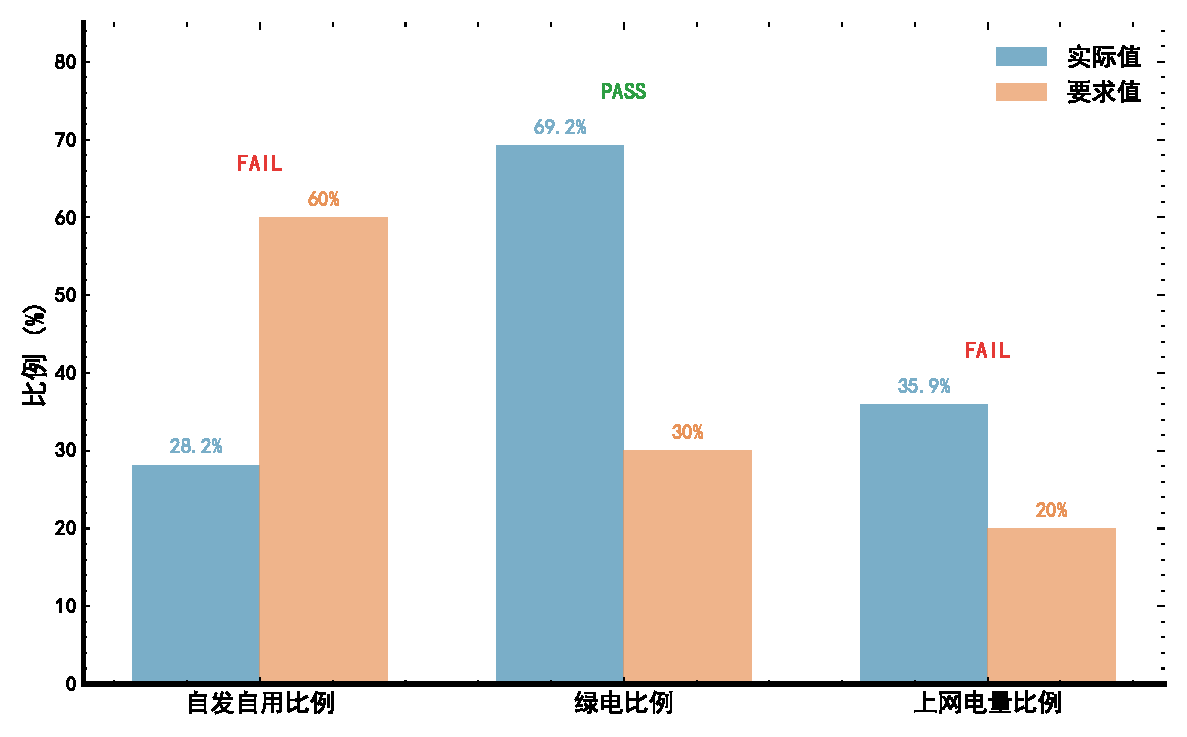
\includegraphics[width=0.75\textwidth]{figures/fig_q1_indicators.pdf}
\caption{绿电直连指标实际值与要求值对比}
\label{fig:q1_indicators}
\end{figure}

% ==================== 问题二 ====================

\begin{figure}[H]
\centering
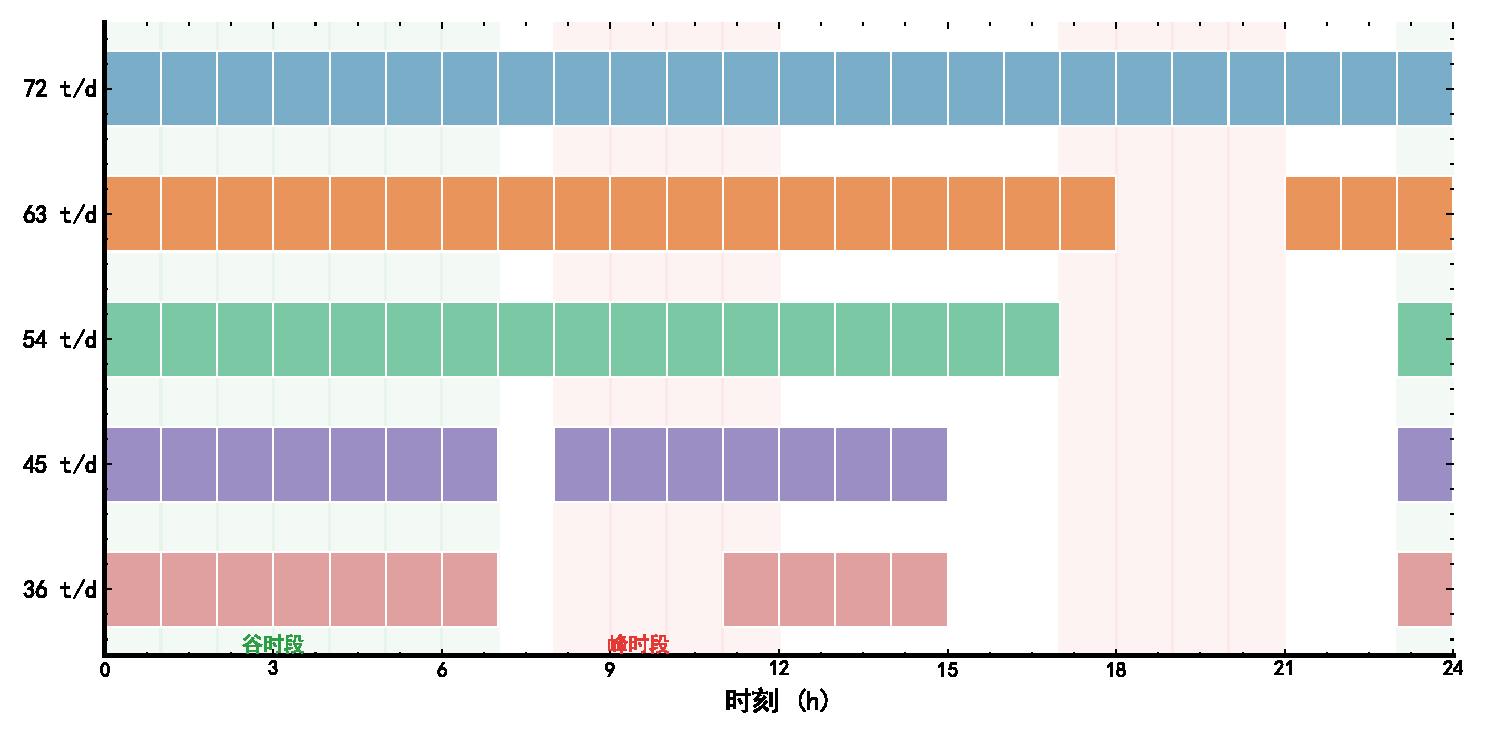
\includegraphics[width=0.92\textwidth]{figures/fig_q2_gantt.pdf}
\caption{不同产量下最优开机时段安排甘特图}
\label{fig:q2_gantt}
\end{figure}

\begin{figure}[H]
\centering
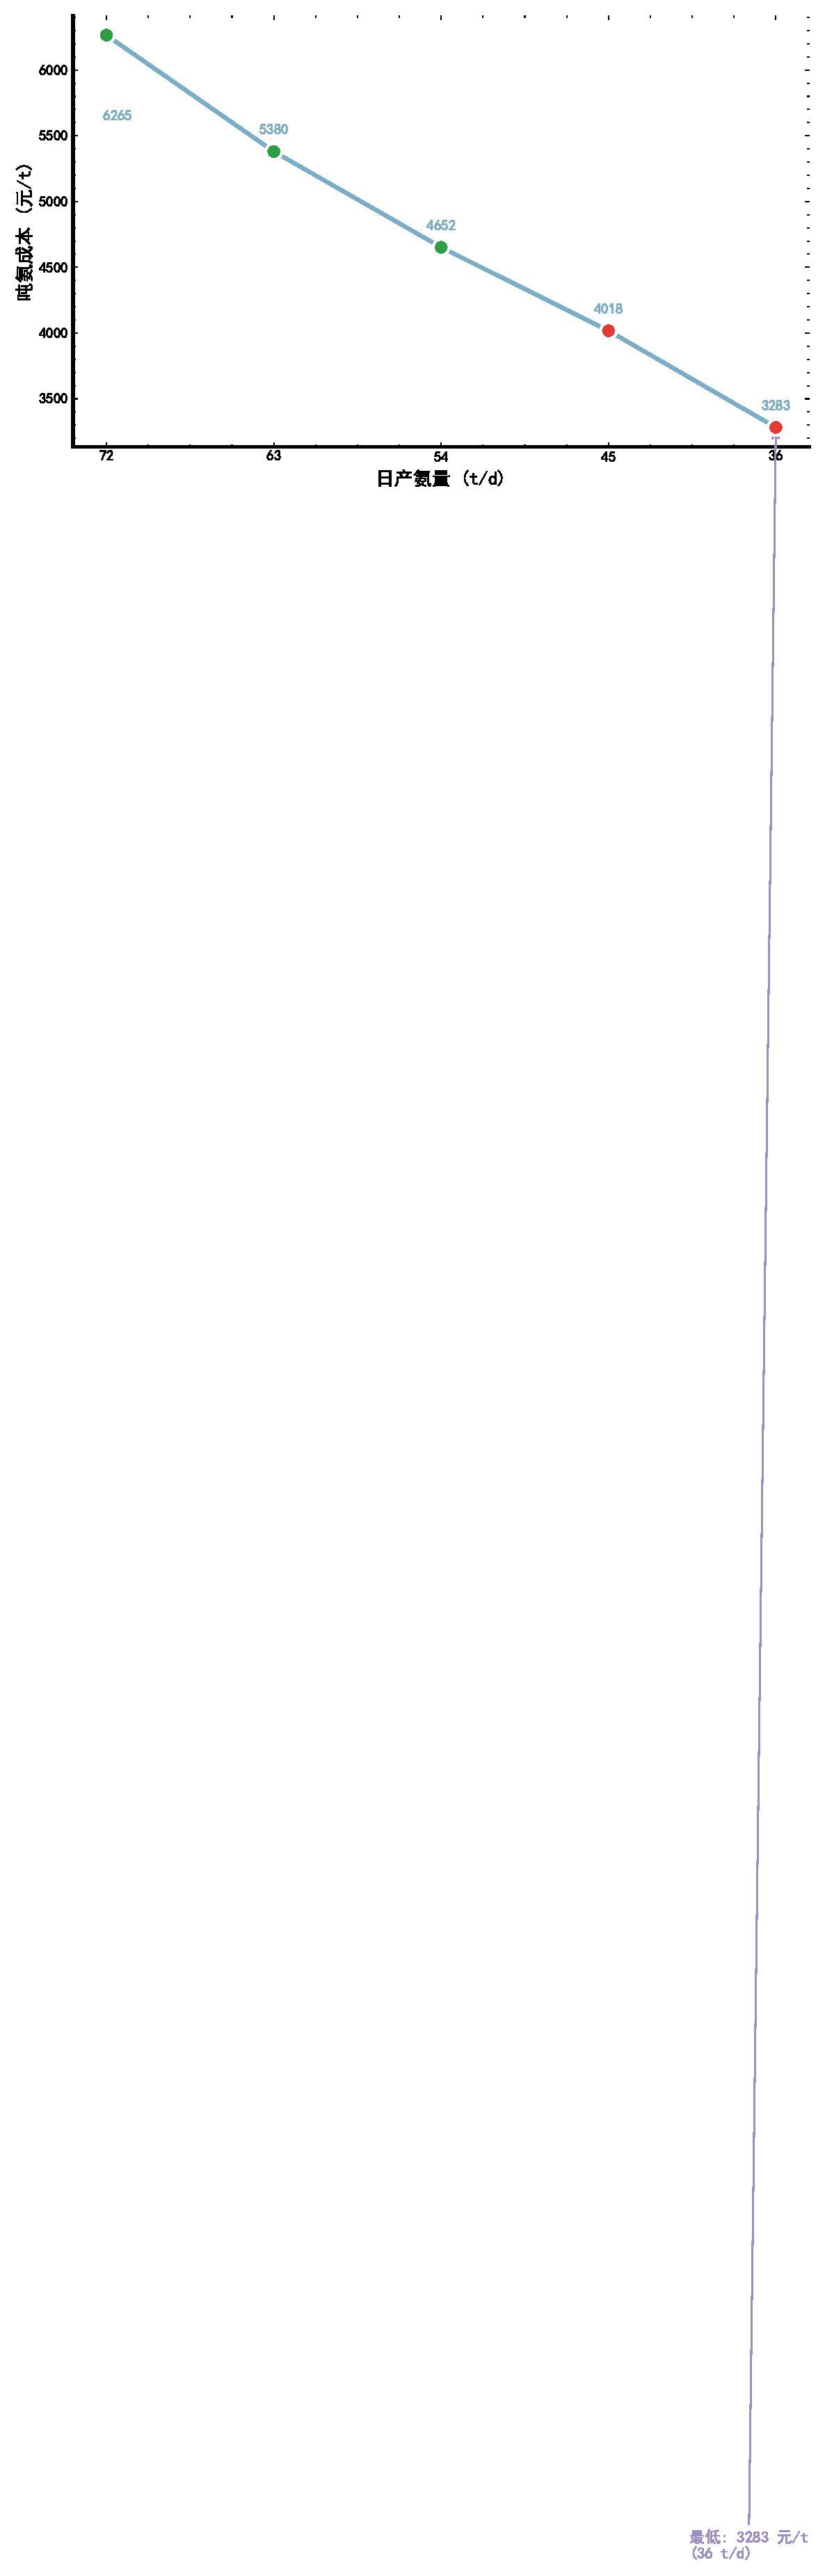
\includegraphics[width=0.78\textwidth]{figures/fig_q2_cost_vs_production.pdf}
\caption{吨氨成本随日产量变化曲线}
\label{fig:q2_cost_vs_production}
\end{figure}

\begin{figure}[H]
\centering
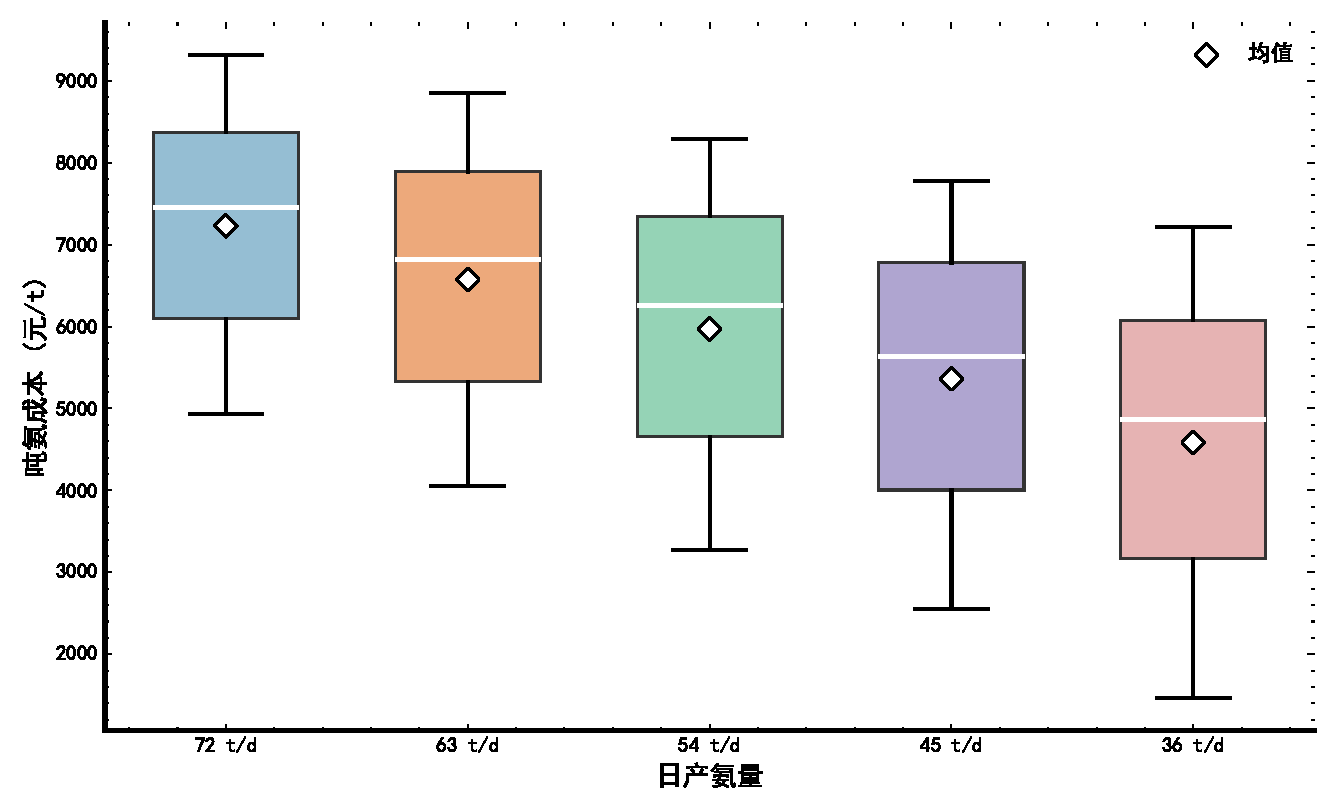
\includegraphics[width=0.82\textwidth]{figures/fig_q2_24scenes_cost.pdf}
\caption{24种风光场景下各产量吨氨成本分布箱线图}
\label{fig:q2_24scenes_cost}
\end{figure}

\begin{figure}[H]
\centering
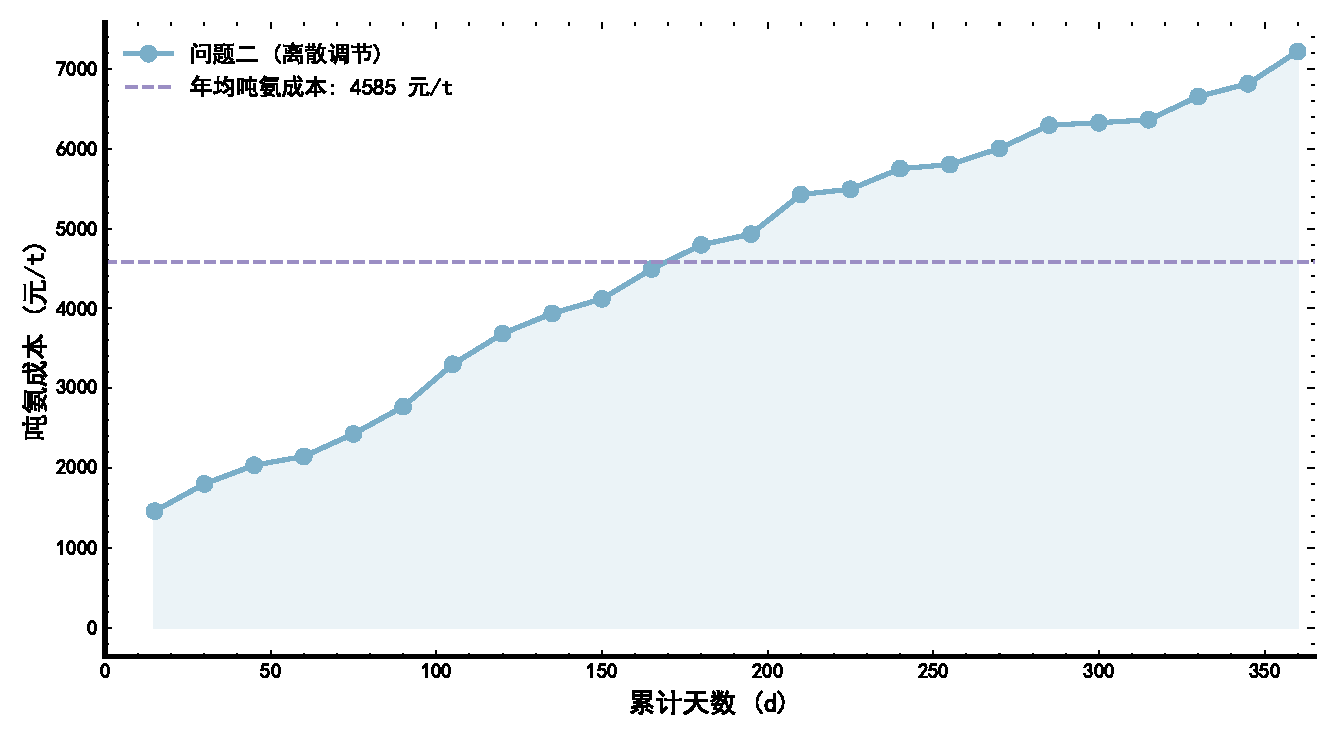
\includegraphics[width=0.85\textwidth]{figures/fig_q2_annual_cost.pdf}
\caption{全年吨氨成本分布曲线（问题二，离散调节，36 t/d）}
\label{fig:q2_annual_cost}
\end{figure}

\begin{figure}[H]
\centering
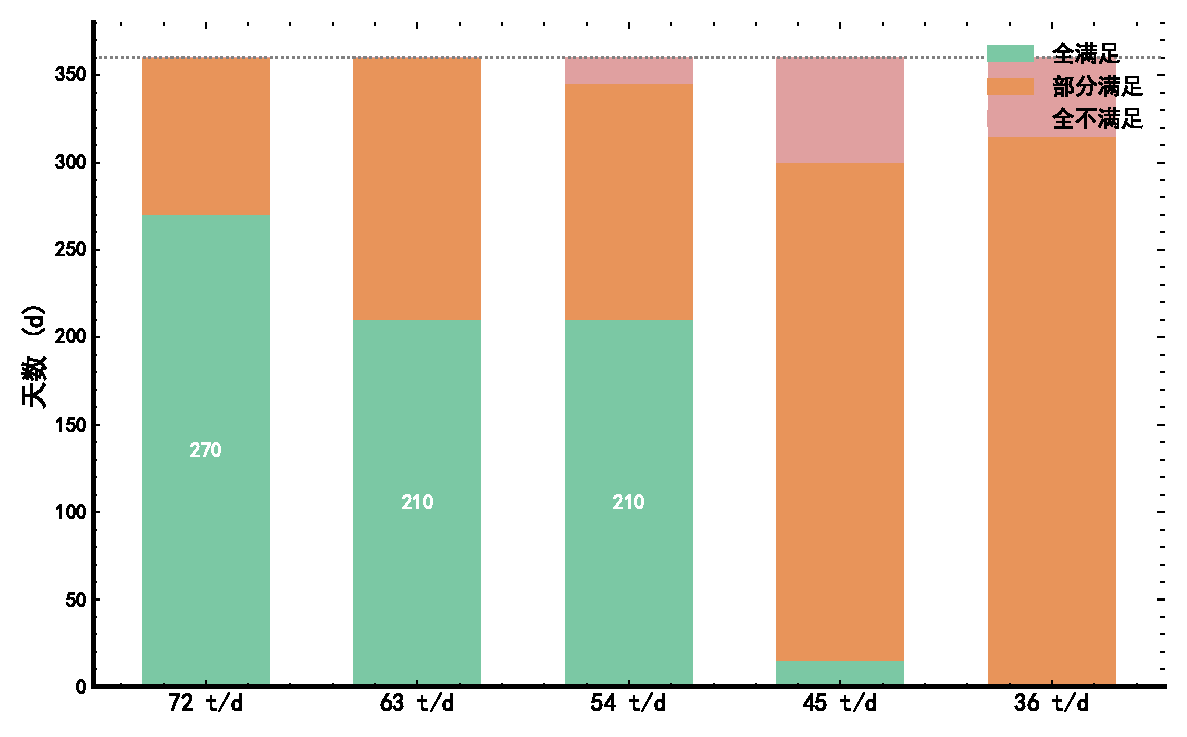
\includegraphics[width=0.78\textwidth]{figures/fig_q2_indicator_stats.pdf}
\caption{全年绿电直连指标满足情况统计}
\label{fig:q2_indicator_stats}
\end{figure}

% ==================== 问题三 ====================

\begin{figure}[H]
\centering
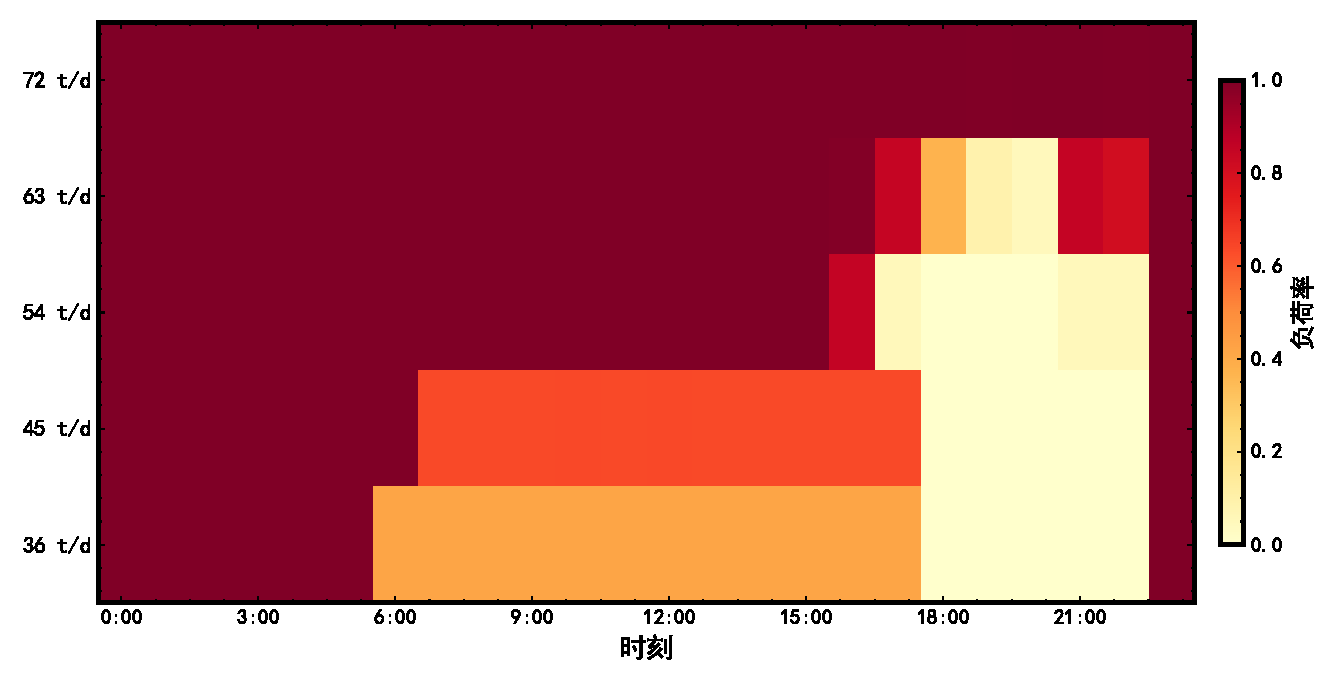
\includegraphics[width=0.92\textwidth]{figures/fig_q3_dispatch.pdf}
\caption{连续调节模式下各产量典型场景负荷率调度热力图}
\label{fig:q3_dispatch}
\end{figure}

\begin{figure}[H]
\centering
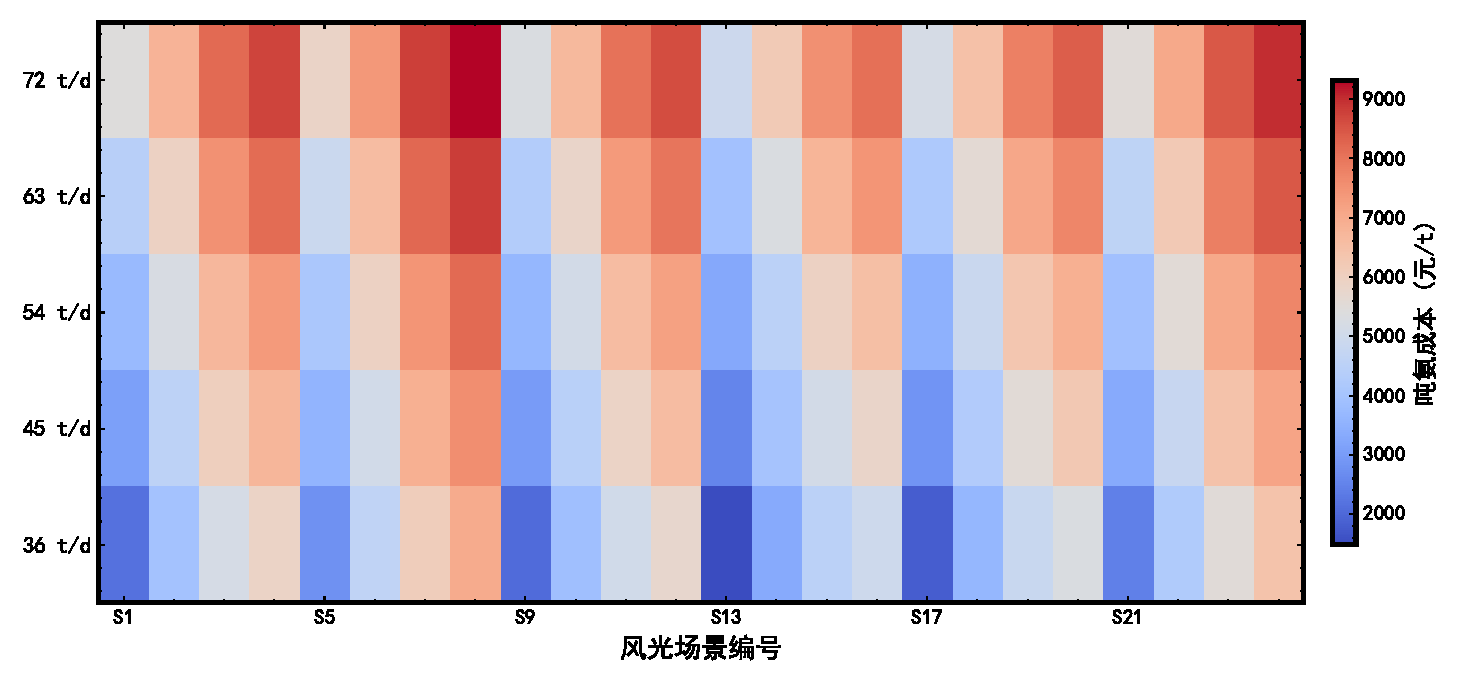
\includegraphics[width=0.92\textwidth]{figures/fig_q3_alpha_heatmap.pdf}
\caption{24种场景下各产量吨氨成本热力图}
\label{fig:q3_alpha_heatmap}
\end{figure}

\begin{figure}[H]
\centering
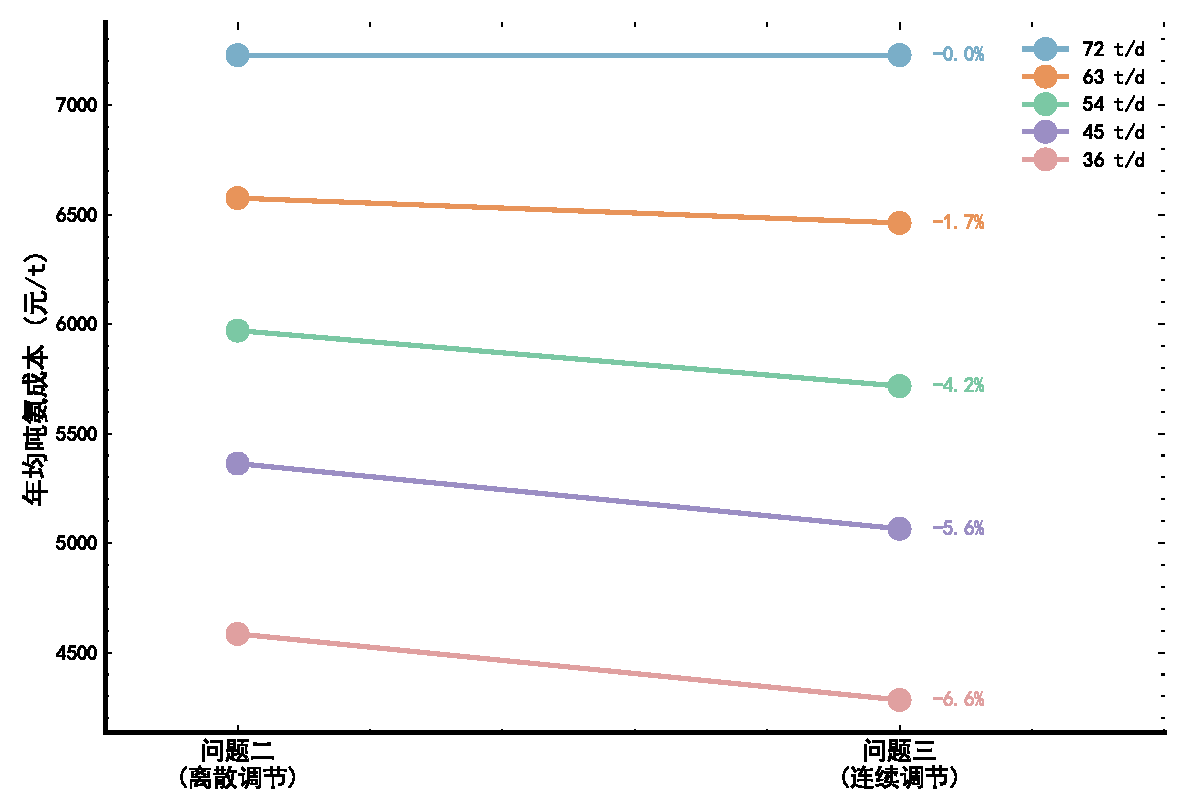
\includegraphics[width=0.78\textwidth]{figures/fig_q3_compare_q2.pdf}
\caption{问题三与问题二年均吨氨成本配对对比图}
\label{fig:q3_compare_q2}
\end{figure}

\begin{figure}[H]
\centering
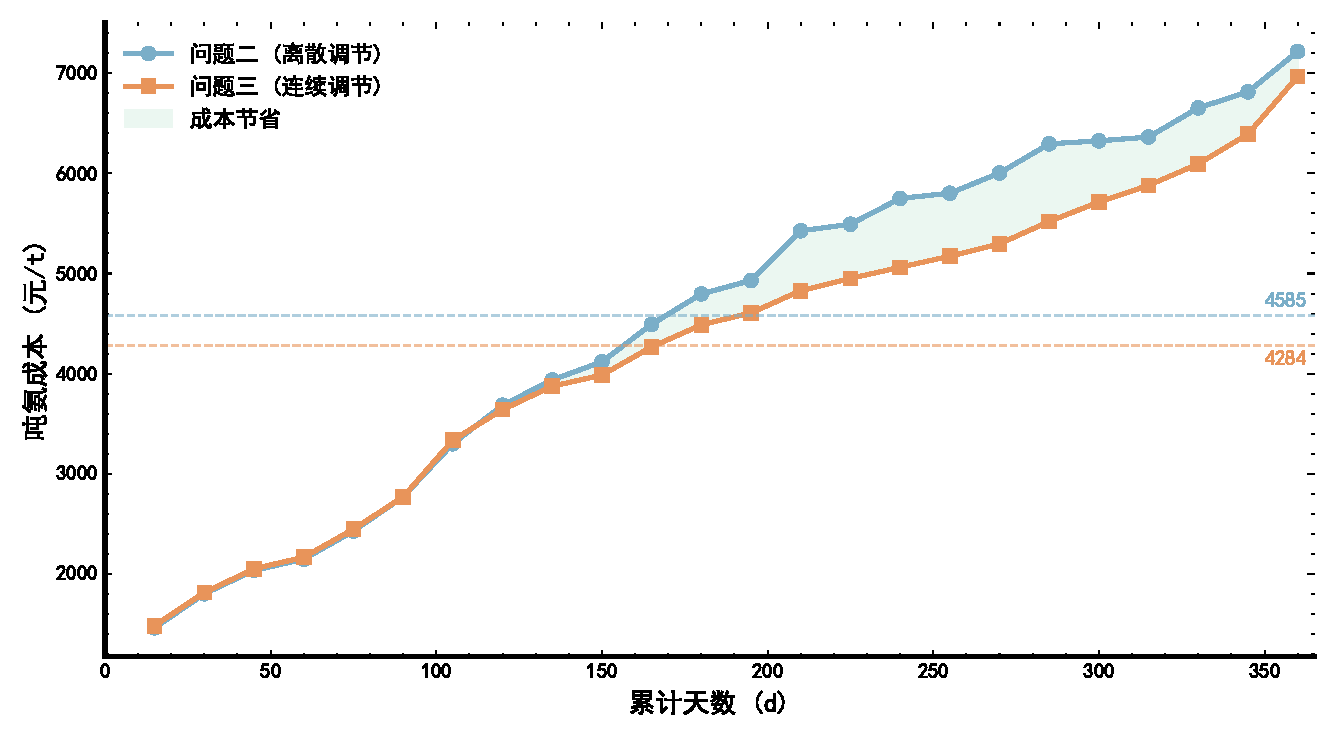
\includegraphics[width=0.85\textwidth]{figures/fig_q3_annual_cost.pdf}
\caption{全年吨氨成本分布曲线（问题二与问题三对比）}
\label{fig:q3_annual_cost}
\end{figure}

% ==================== 问题四 ====================

\begin{figure}[H]
\centering
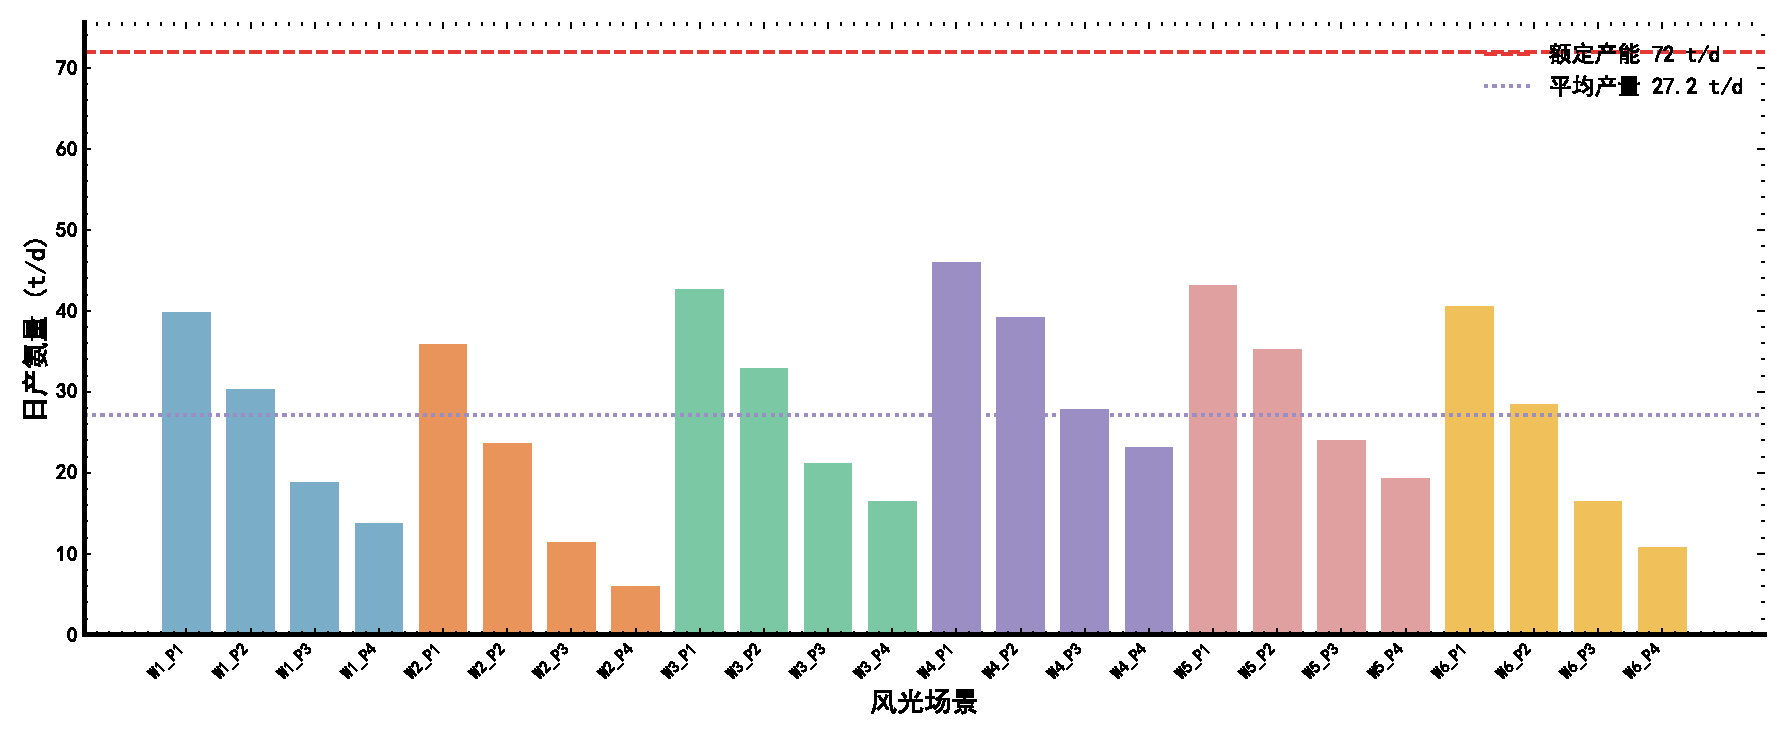
\includegraphics[width=0.95\textwidth]{figures/fig_q4_offgrid_production.pdf}
\caption{24种风光场景下离网运行日产氨量}
\label{fig:q4_offgrid_production}
\end{figure}

\begin{figure}[H]
\centering
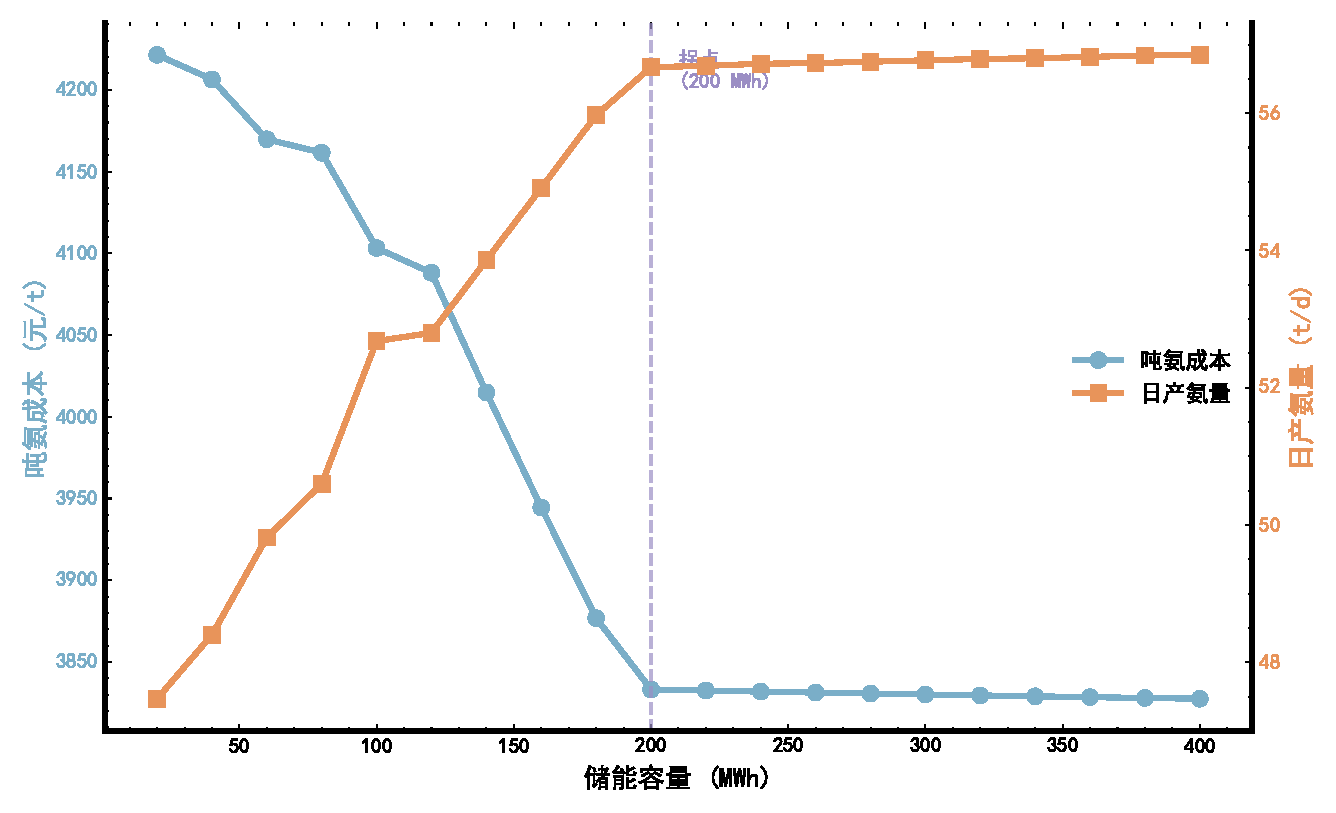
\includegraphics[width=0.82\textwidth]{figures/fig_q4_storage_optimization.pdf}
\caption{储能容量与吨氨成本、日产氨量关系曲线}
\label{fig:q4_storage_optimization}
\end{figure}

\begin{figure}[H]
\centering
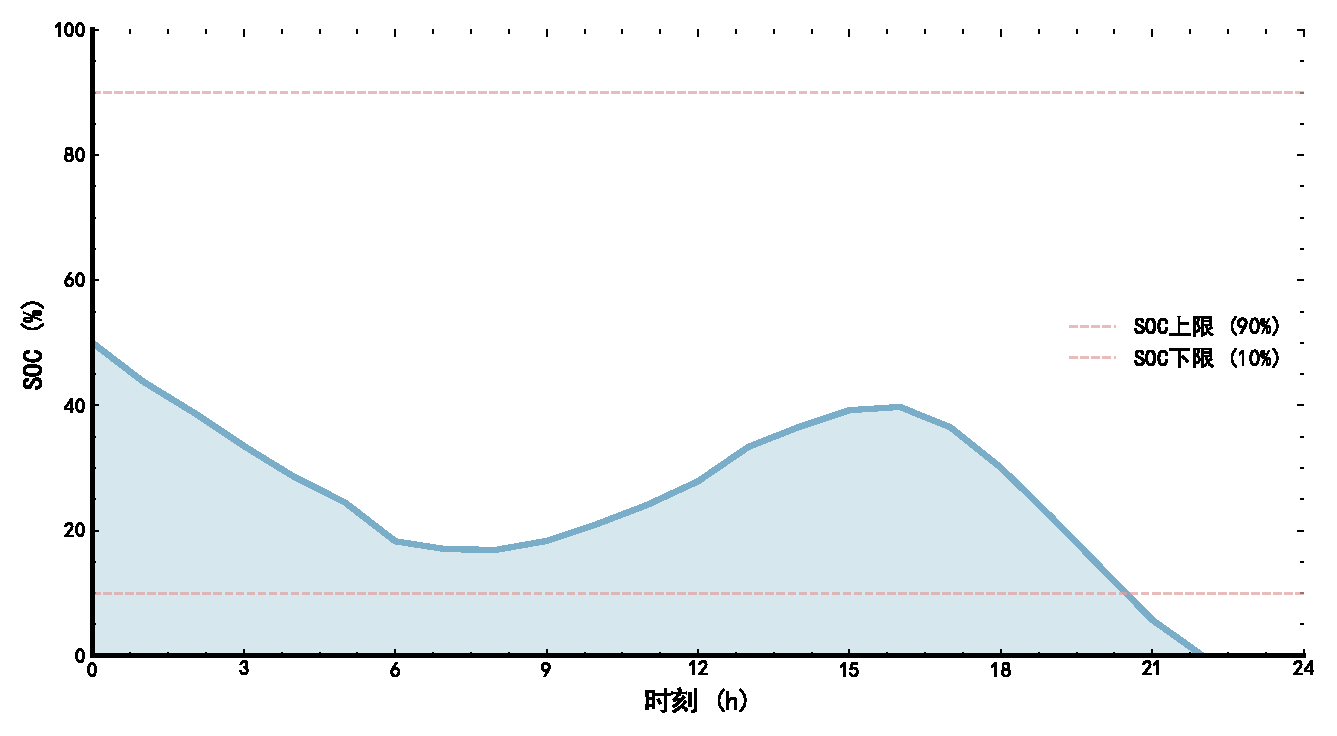
\includegraphics[width=0.82\textwidth]{figures/fig_q4_soc_curve.pdf}
\caption{最大弃电场景储能SOC变化曲线}
\label{fig:q4_soc_curve}
\end{figure}

\begin{figure}[H]
\centering
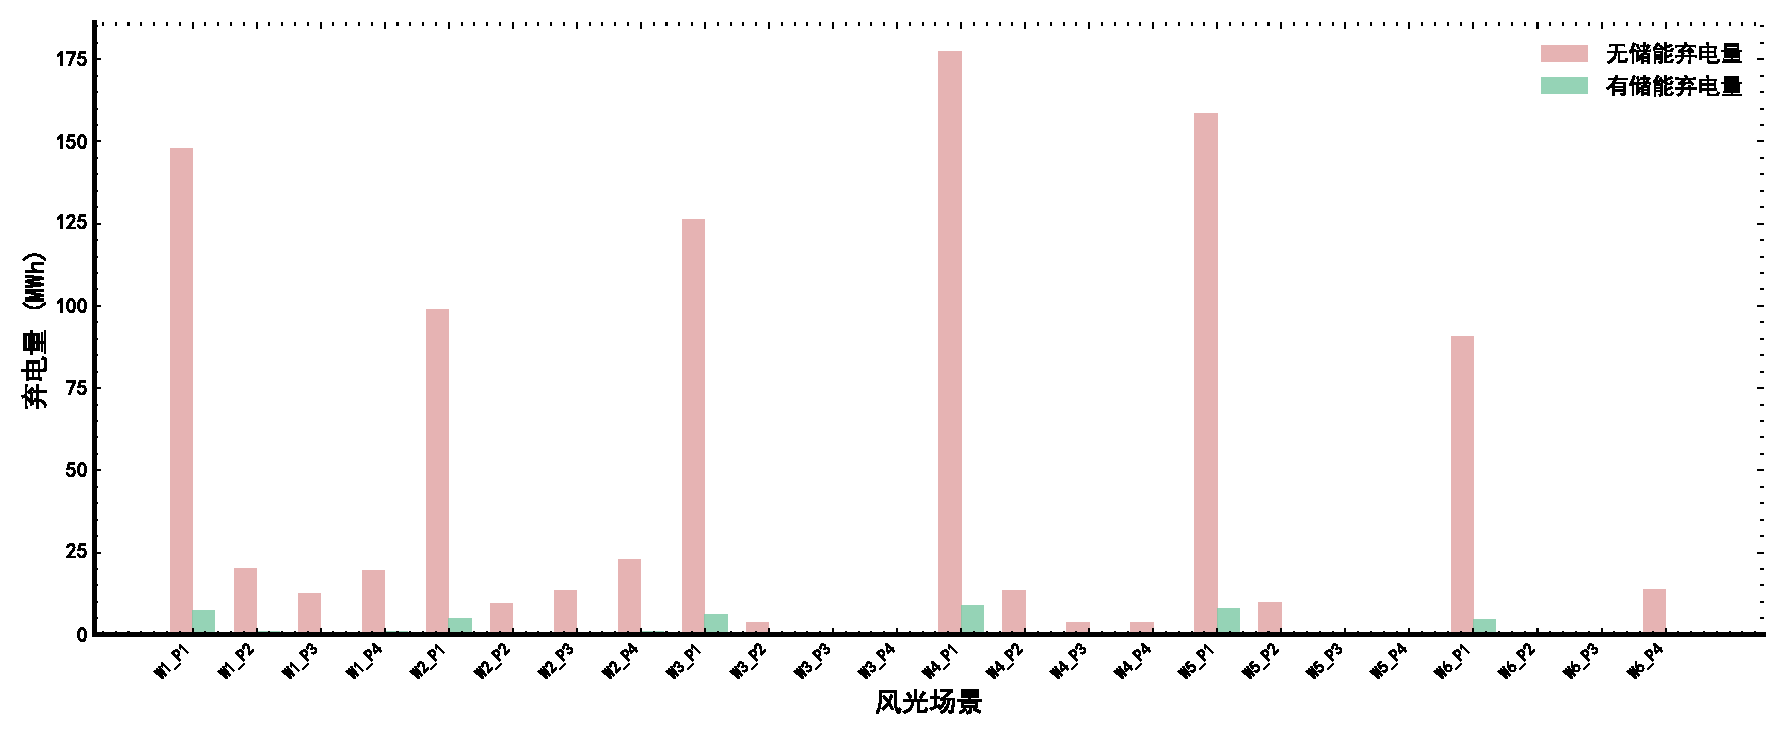
\includegraphics[width=0.95\textwidth]{figures/fig_q4_curtail_compare.pdf}
\caption{有无储能弃电量对比}
\label{fig:q4_curtail_compare}
\end{figure}

\begin{figure}[H]
\centering
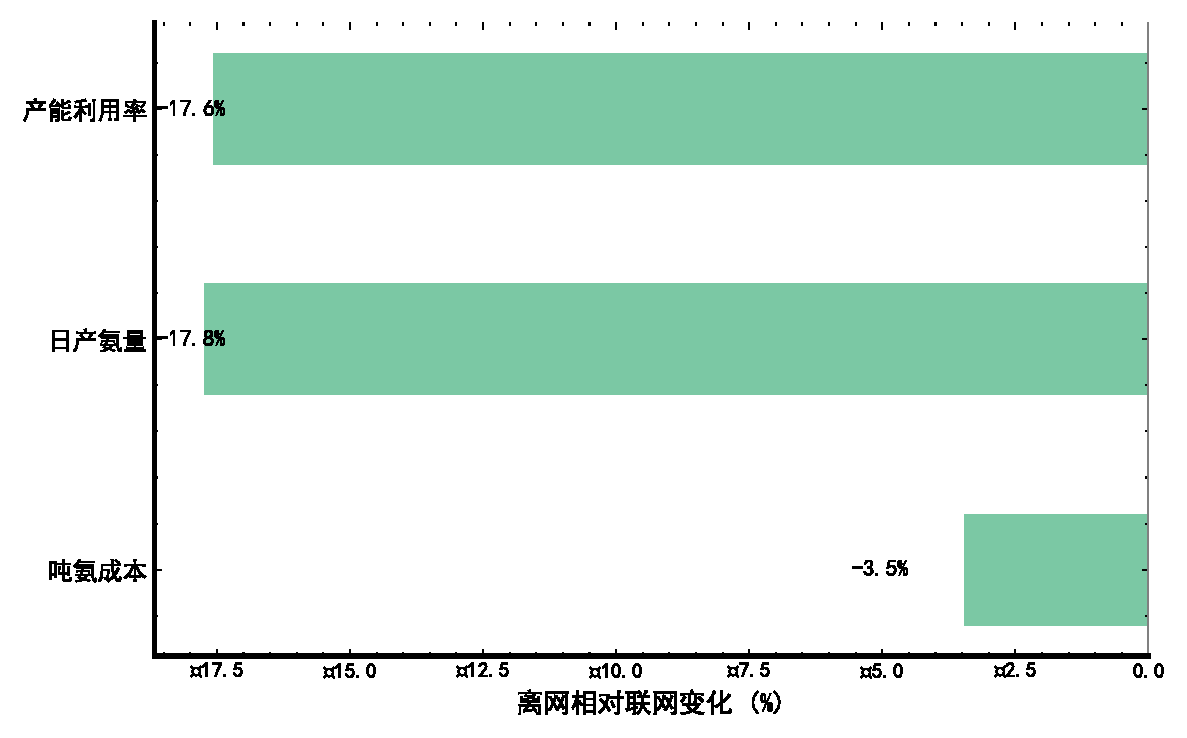
\includegraphics[width=0.75\textwidth]{figures/fig_q4_onoff_compare.pdf}
\caption{离网与联网运行模式经济性对比（发散柱状图）}
\label{fig:q4_onoff_compare}
\end{figure}

% ==================== 灵敏度分析 ====================

\begin{figure}[H]
\centering
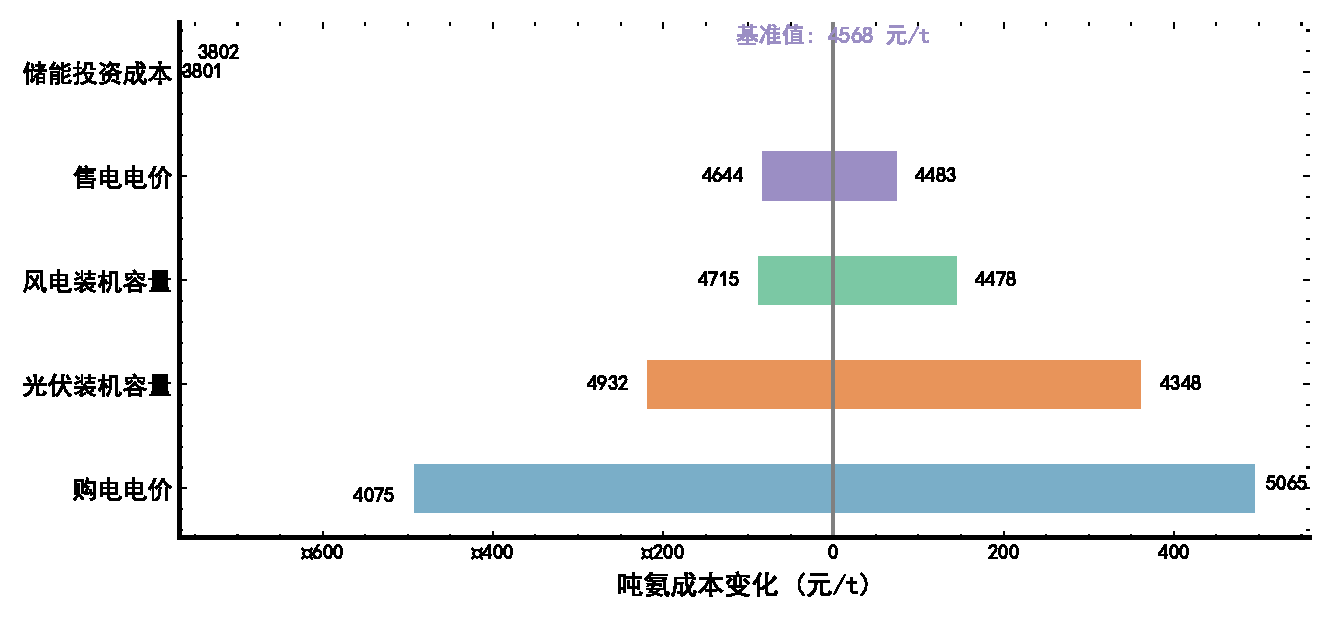
\includegraphics[width=0.82\textwidth]{figures/fig_sensitivity.pdf}
\caption{关键参数敏感性分析龙卷风图}
\label{fig:sensitivity}
\end{figure}

% ============================================================

% ==================== 技术路线图 ====================

\begin{figure}[H]
\centering
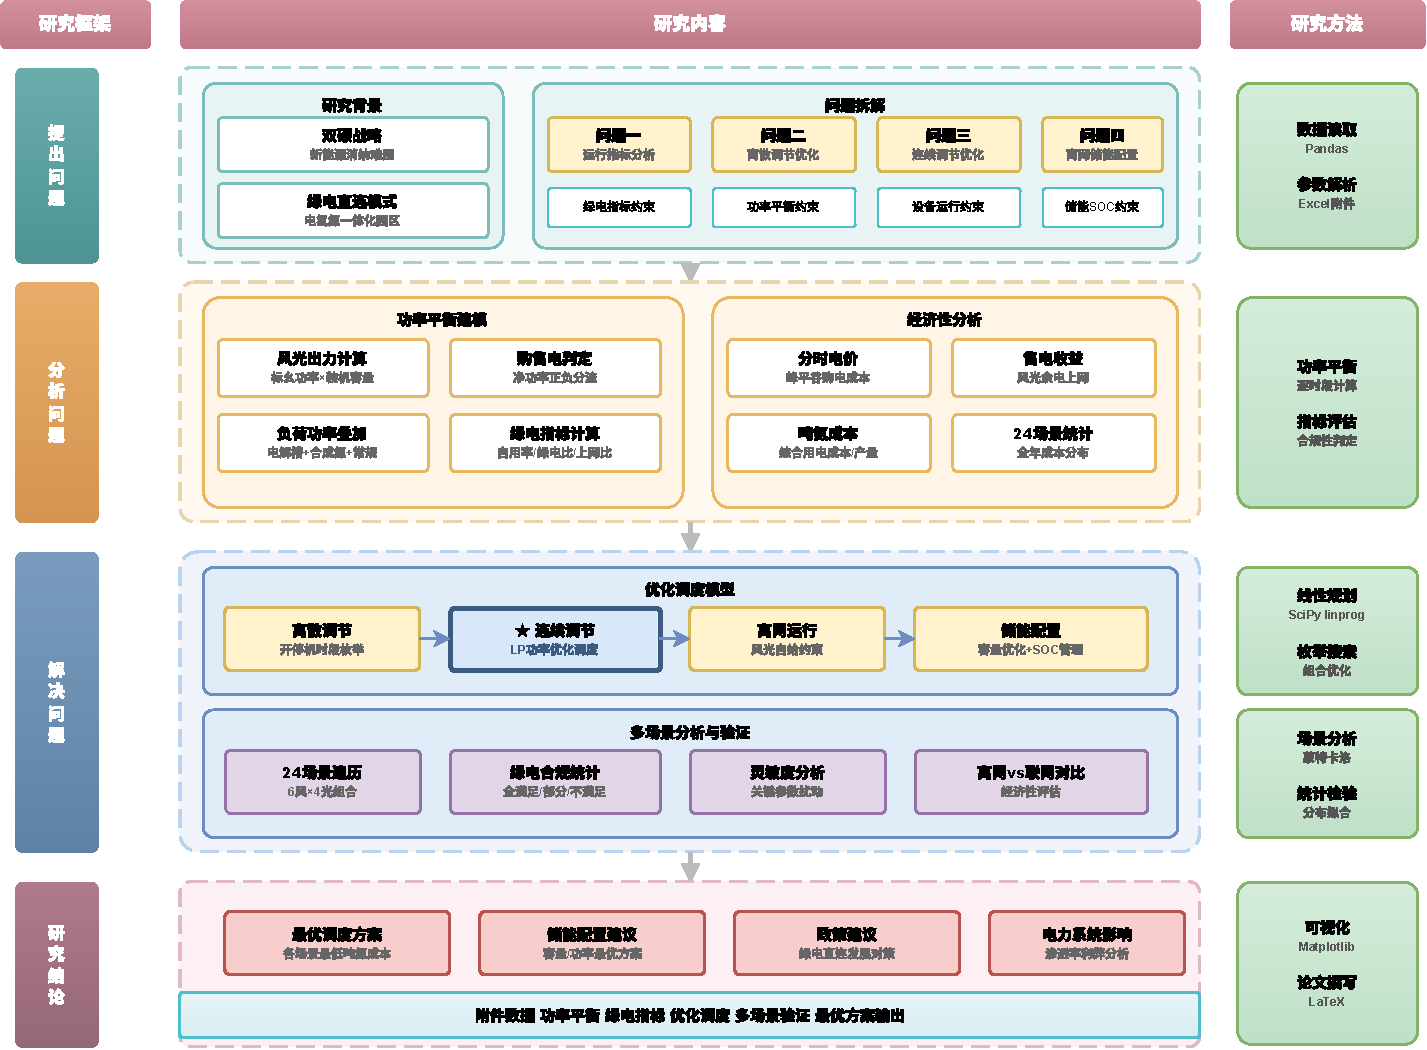
\includegraphics[width=\textwidth,height=0.45\textheight,keepaspectratio]{figures/fig_roadmap.pdf}
\caption{整体技术路线图}\label{fig:roadmap}
\end{figure}

% ==================== 园区系统架构图 ====================

\begin{figure}[H]
\centering
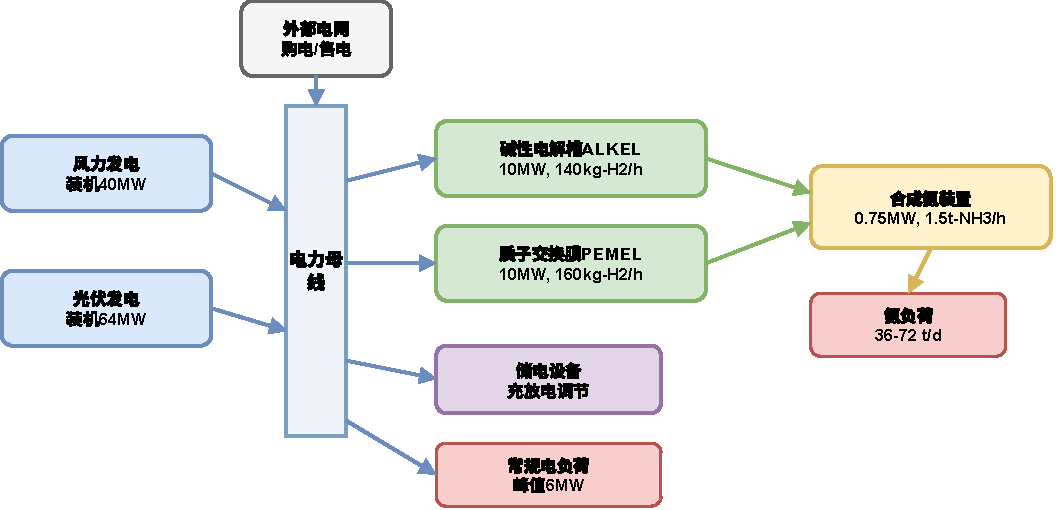
\includegraphics[width=0.9\textwidth,height=0.3\textheight,keepaspectratio]{figures/fig_system_arch.pdf}
\caption{绿电直连型电氢氨园区系统架构}\label{fig:system_arch}
\end{figure}

% ==================== 求解流程图 ====================

\begin{figure}[H]
\centering
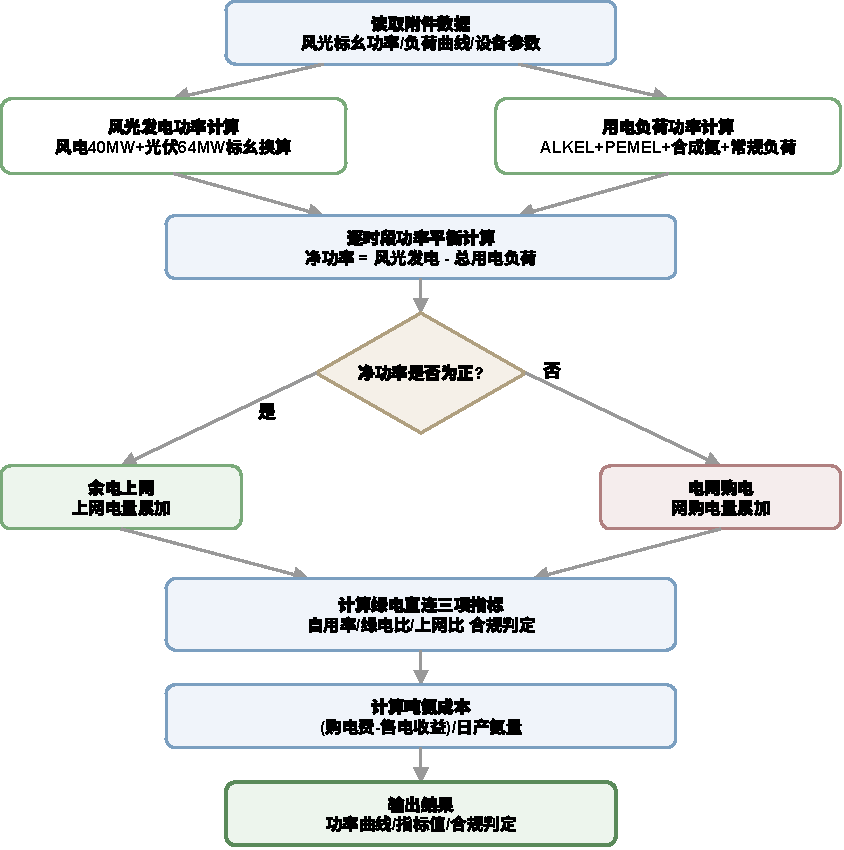
\includegraphics[width=0.85\textwidth,height=0.38\textheight,keepaspectratio]{figures/fig_flow_q1.pdf}
\caption{问题一求解流程图}\label{fig:flow_q1}
\end{figure}

\begin{figure}[H]
\centering
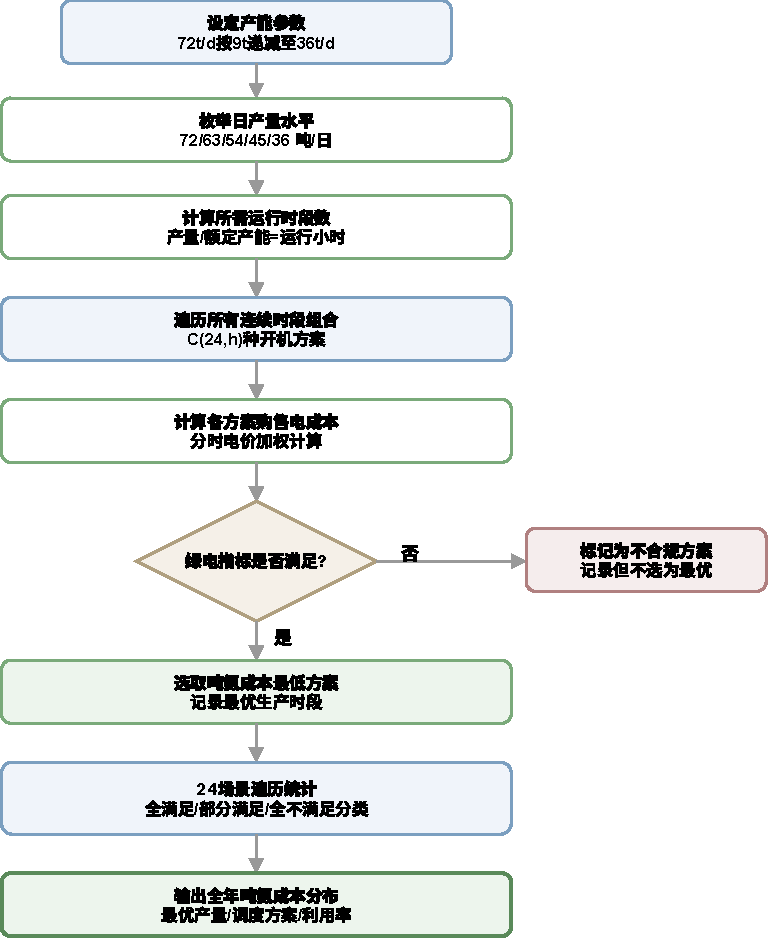
\includegraphics[width=0.85\textwidth,height=0.38\textheight,keepaspectratio]{figures/fig_flow_q2.pdf}
\caption{问题二求解流程图}\label{fig:flow_q2}
\end{figure}

\begin{figure}[H]
\centering
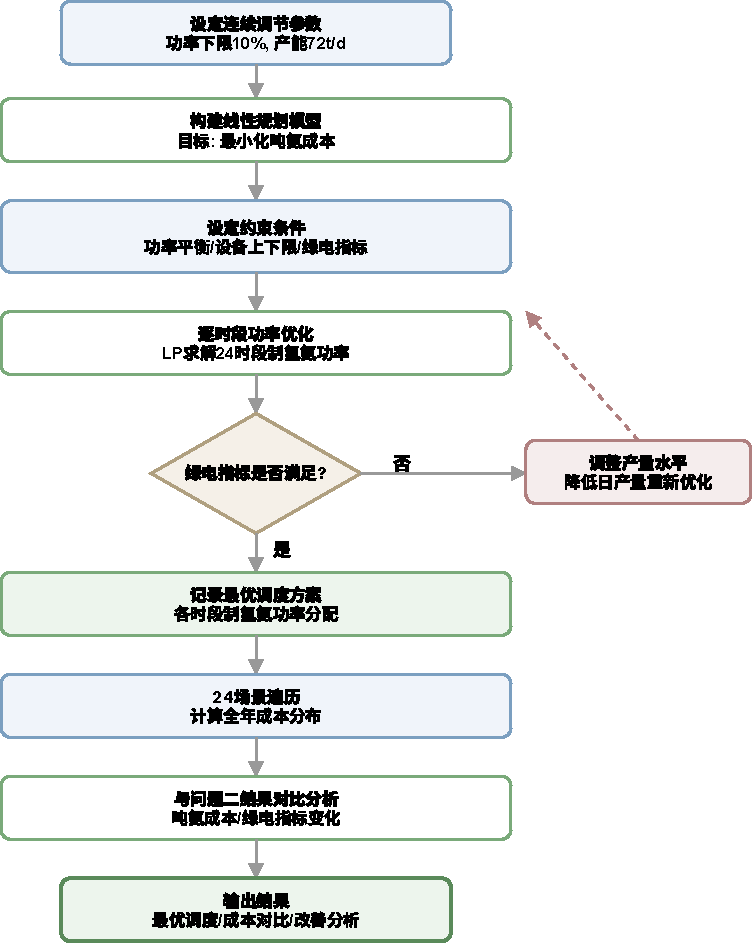
\includegraphics[width=0.85\textwidth,height=0.38\textheight,keepaspectratio]{figures/fig_flow_q3.pdf}
\caption{问题三求解流程图}\label{fig:flow_q3}
\end{figure}

\begin{figure}[H]
\centering
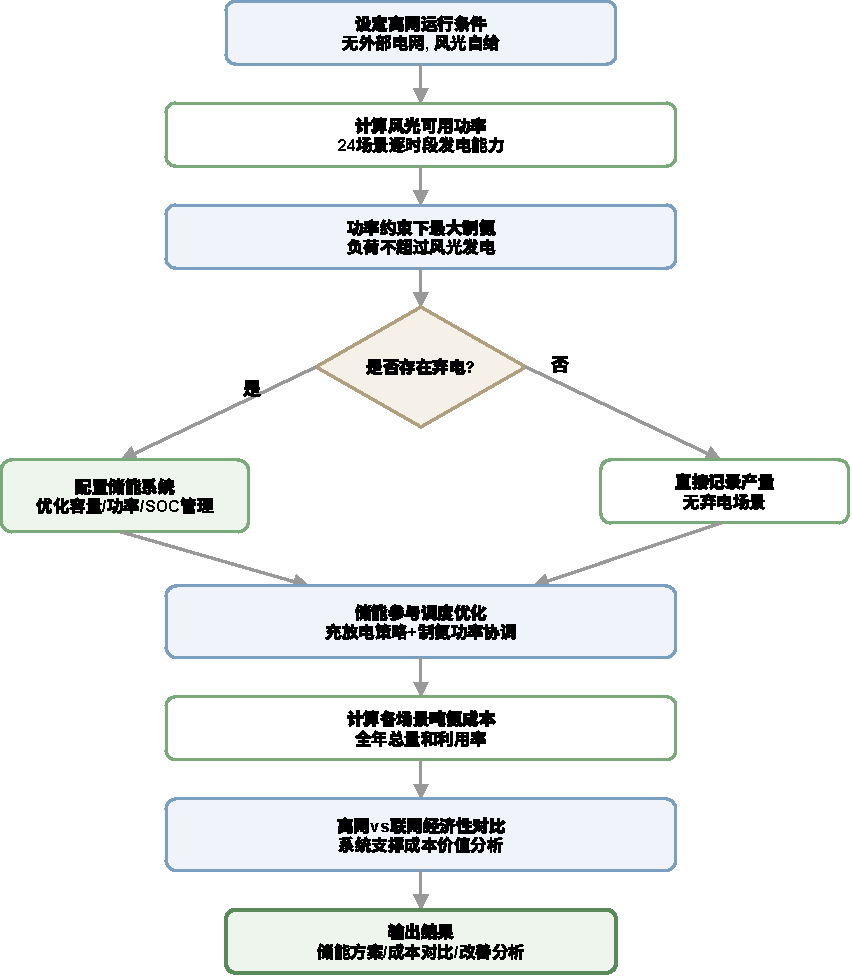
\includegraphics[width=0.85\textwidth,height=0.38\textheight,keepaspectratio]{figures/fig_flow_q4.pdf}
\caption{问题四求解流程图}\label{fig:flow_q4}
\end{figure}

% ==================== 问题一 ====================

\begin{figure}[H]
\centering
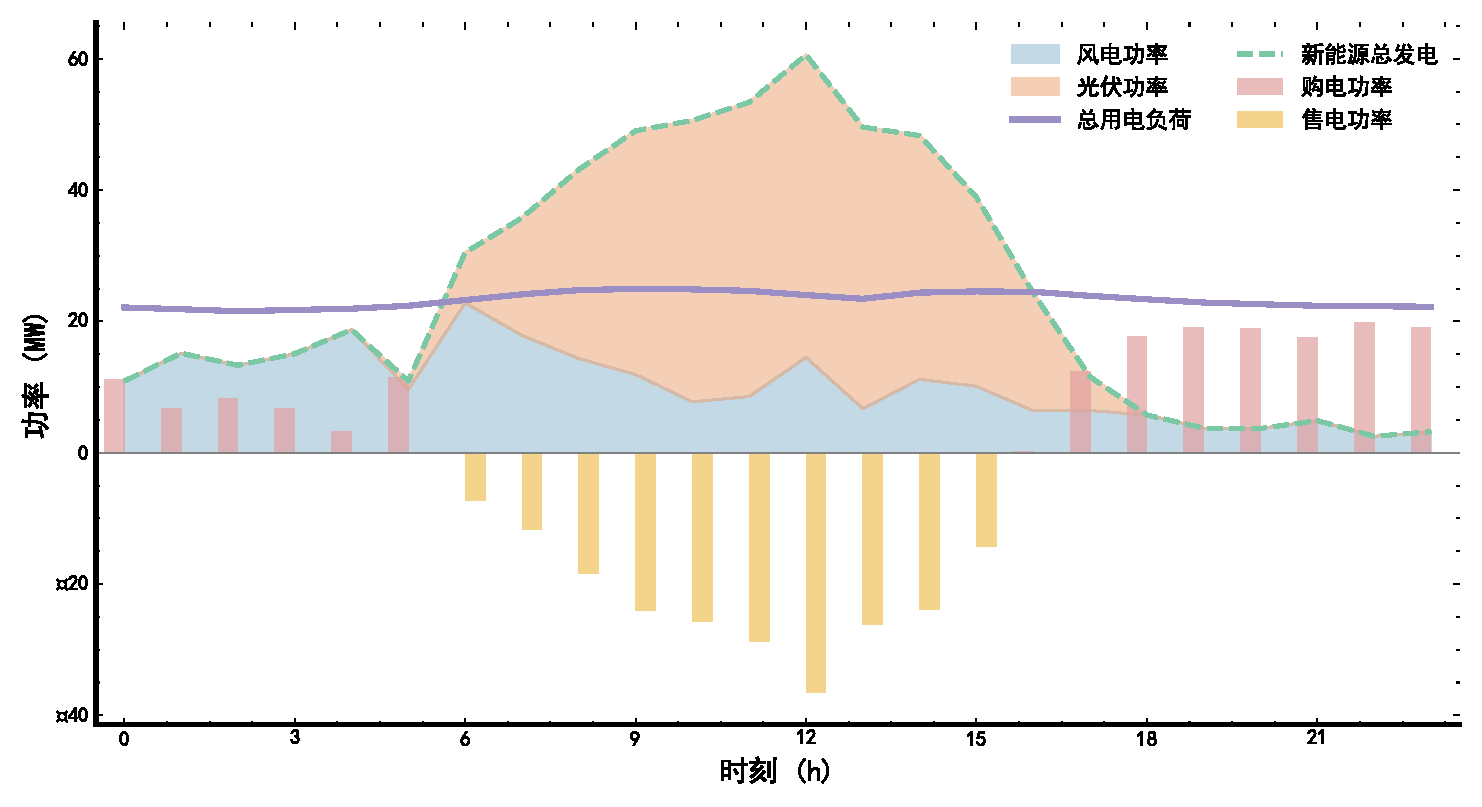
\includegraphics[width=0.95\textwidth]{figures/fig_q1_power_balance.pdf}
\caption{典型日功率平衡曲线（风电、光伏发电与负荷、购售电功率对比）}
\label{fig:q1_power_balance}
\end{figure}

\begin{figure}[H]
\centering
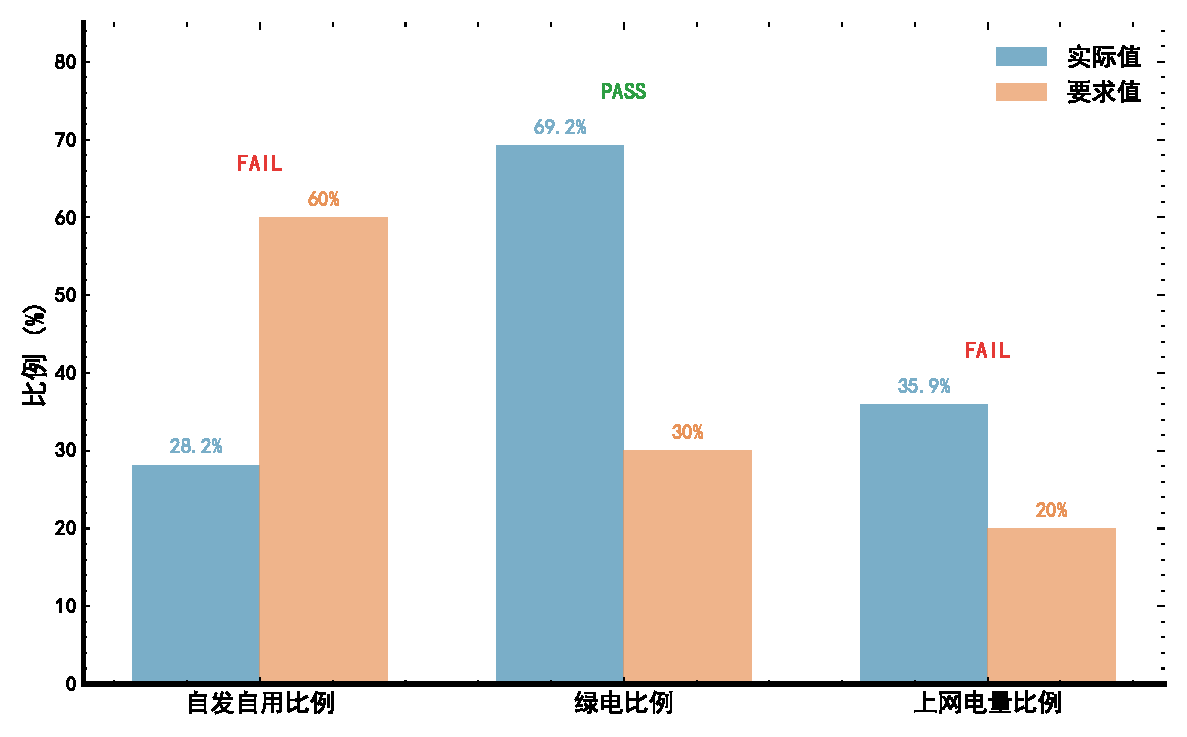
\includegraphics[width=0.75\textwidth]{figures/fig_q1_indicators.pdf}
\caption{绿电直连指标实际值与要求值对比}
\label{fig:q1_indicators}
\end{figure}

% ==================== 问题二 ====================

\begin{figure}[H]
\centering
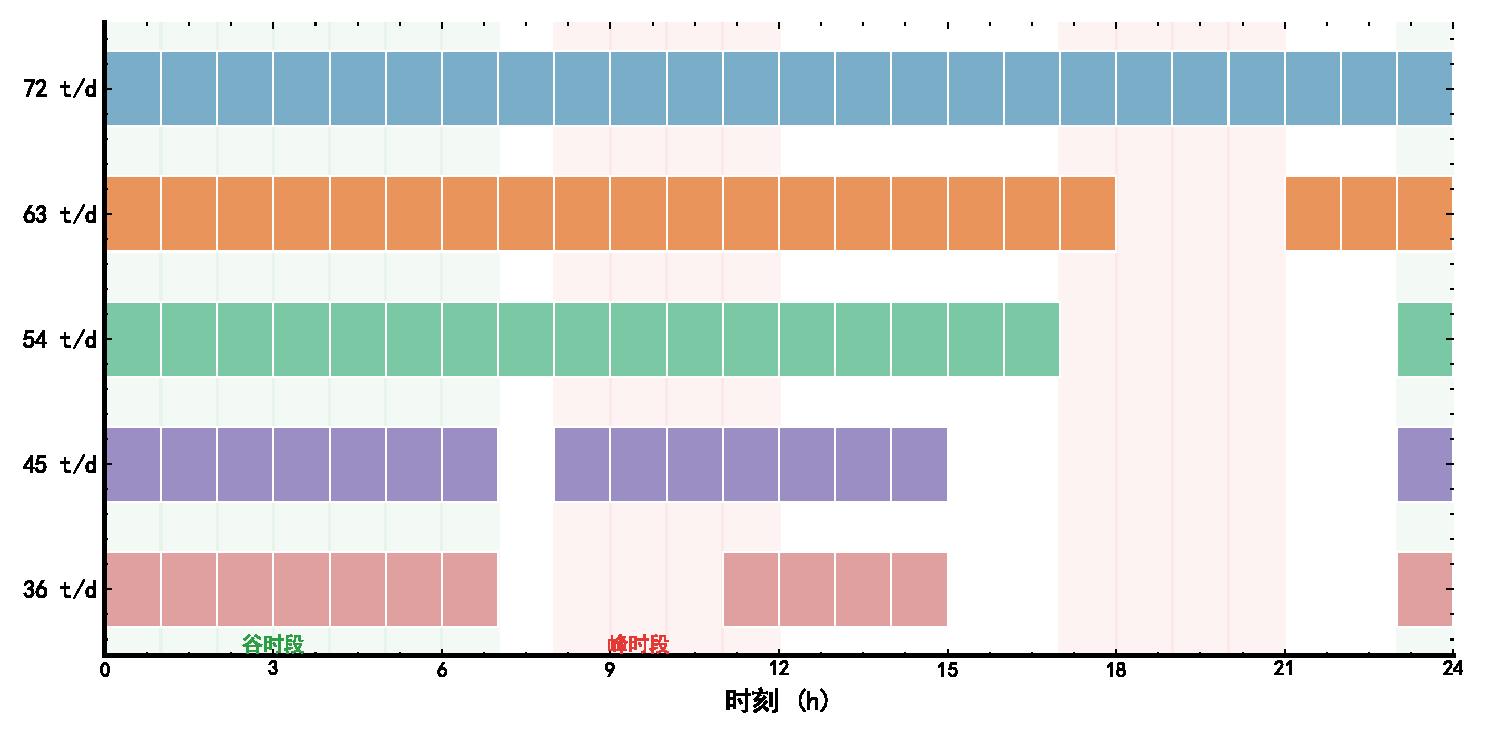
\includegraphics[width=0.92\textwidth]{figures/fig_q2_gantt.pdf}
\caption{不同产量下最优开机时段安排甘特图}
\label{fig:q2_gantt}
\end{figure}

\begin{figure}[H]
\centering
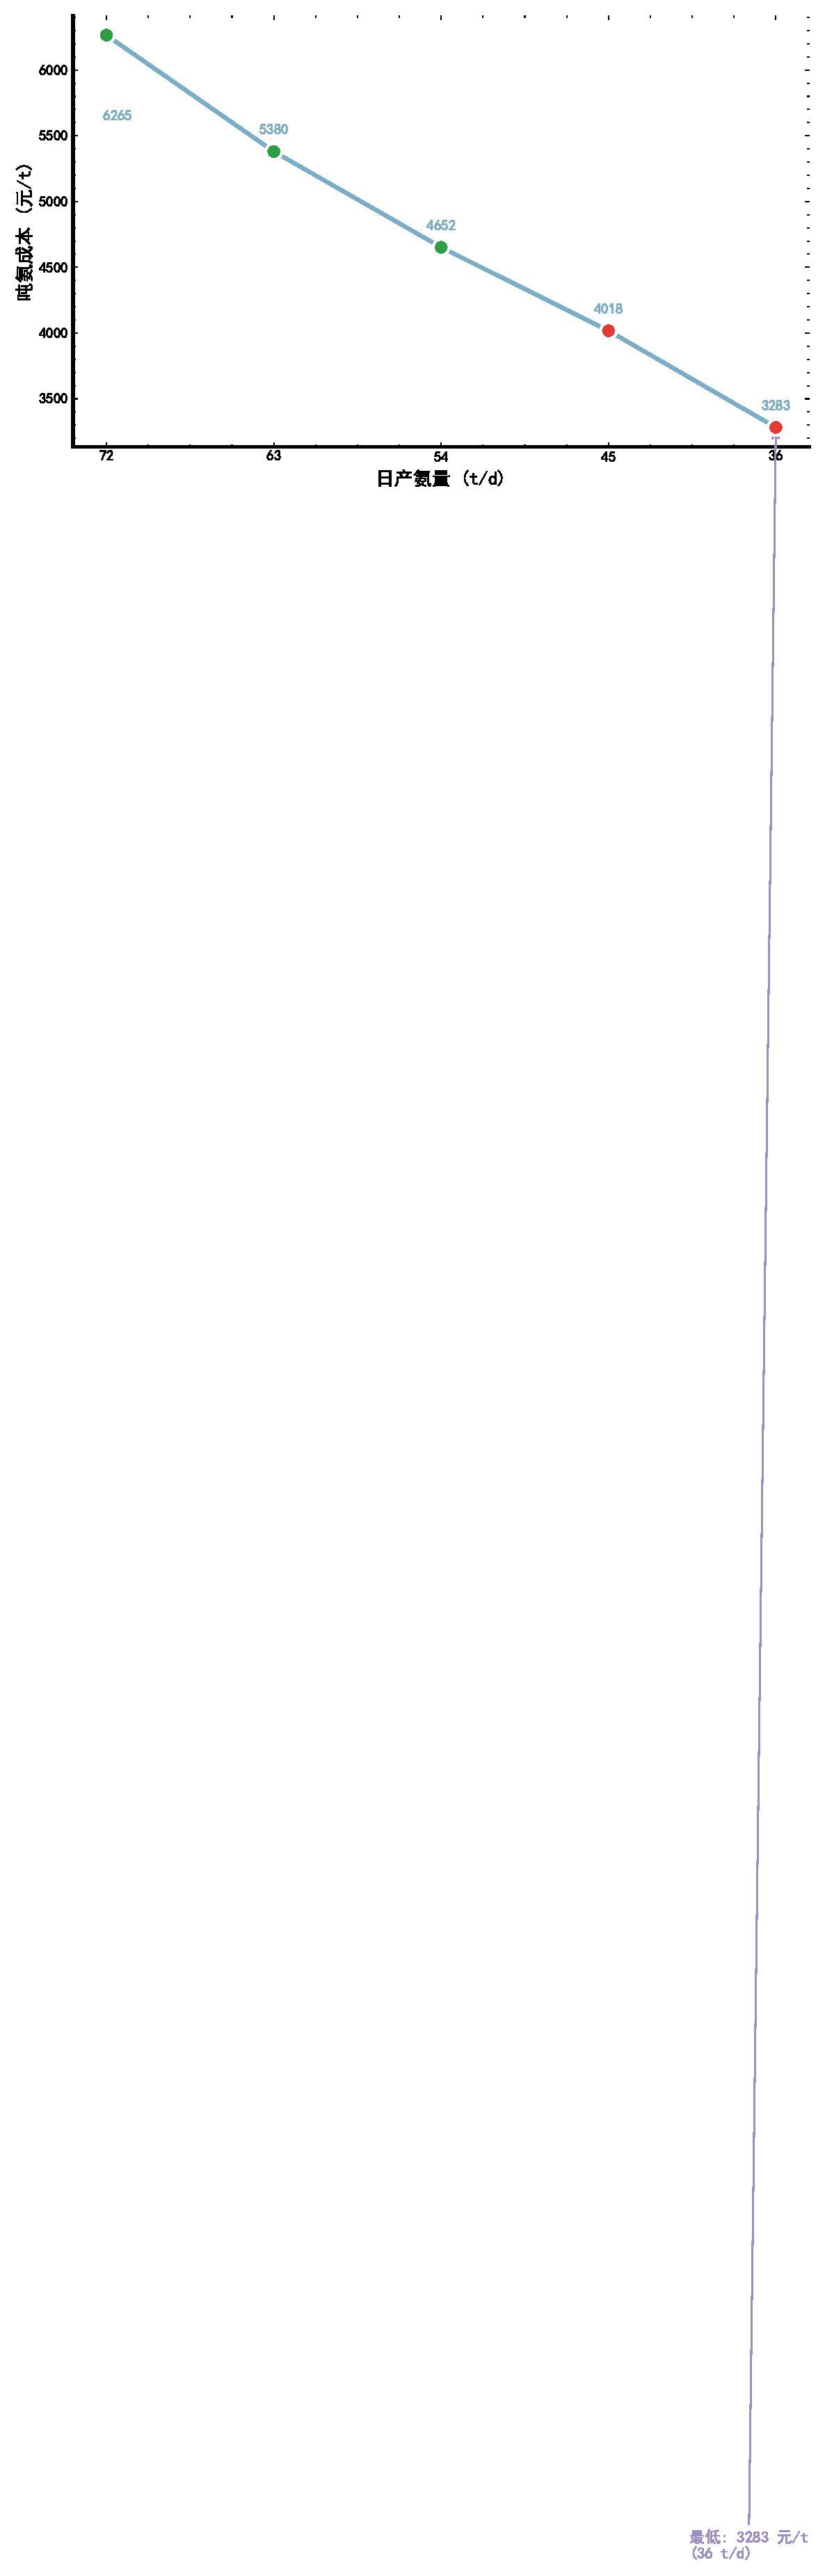
\includegraphics[width=0.78\textwidth]{figures/fig_q2_cost_vs_production.pdf}
\caption{吨氨成本随日产量变化曲线}
\label{fig:q2_cost_vs_production}
\end{figure}

\begin{figure}[H]
\centering
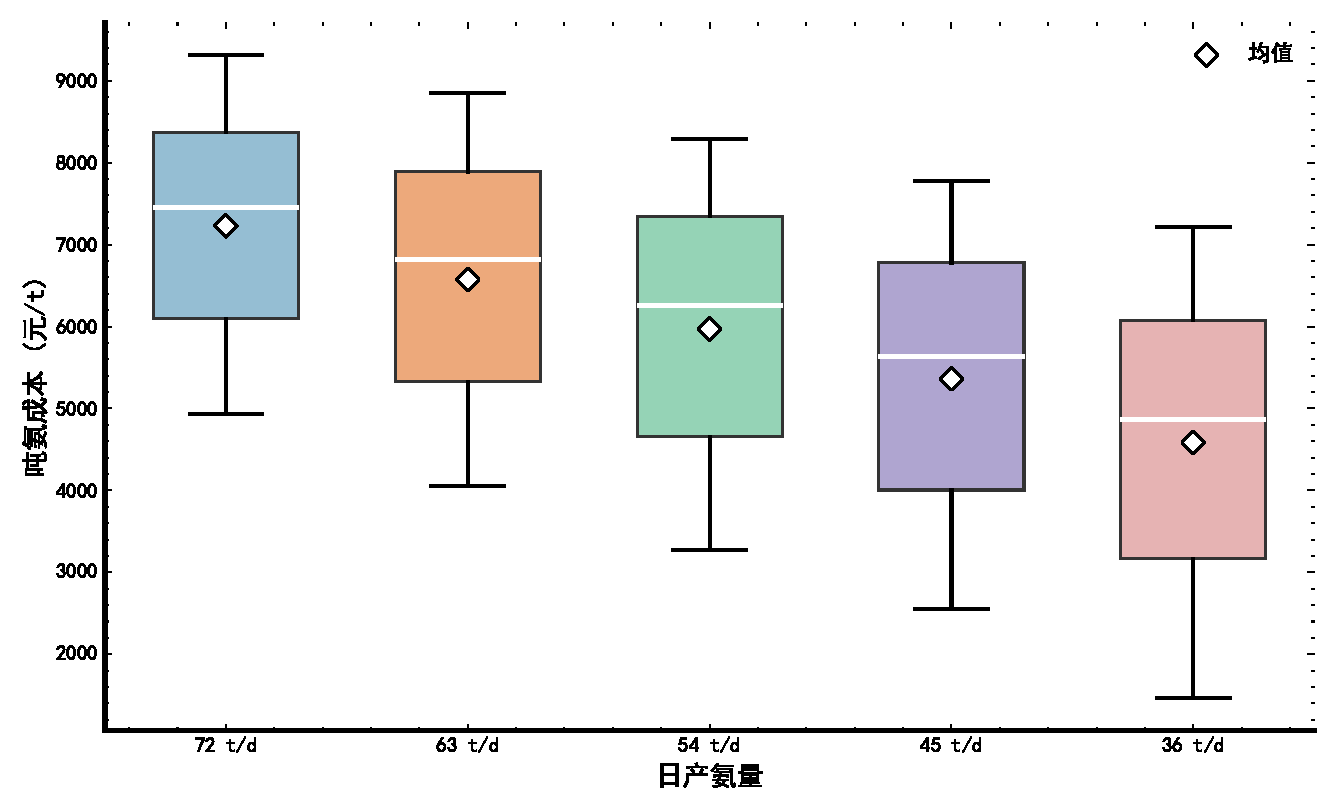
\includegraphics[width=0.82\textwidth]{figures/fig_q2_24scenes_cost.pdf}
\caption{24种风光场景下各产量吨氨成本分布箱线图}
\label{fig:q2_24scenes_cost}
\end{figure}

\begin{figure}[H]
\centering
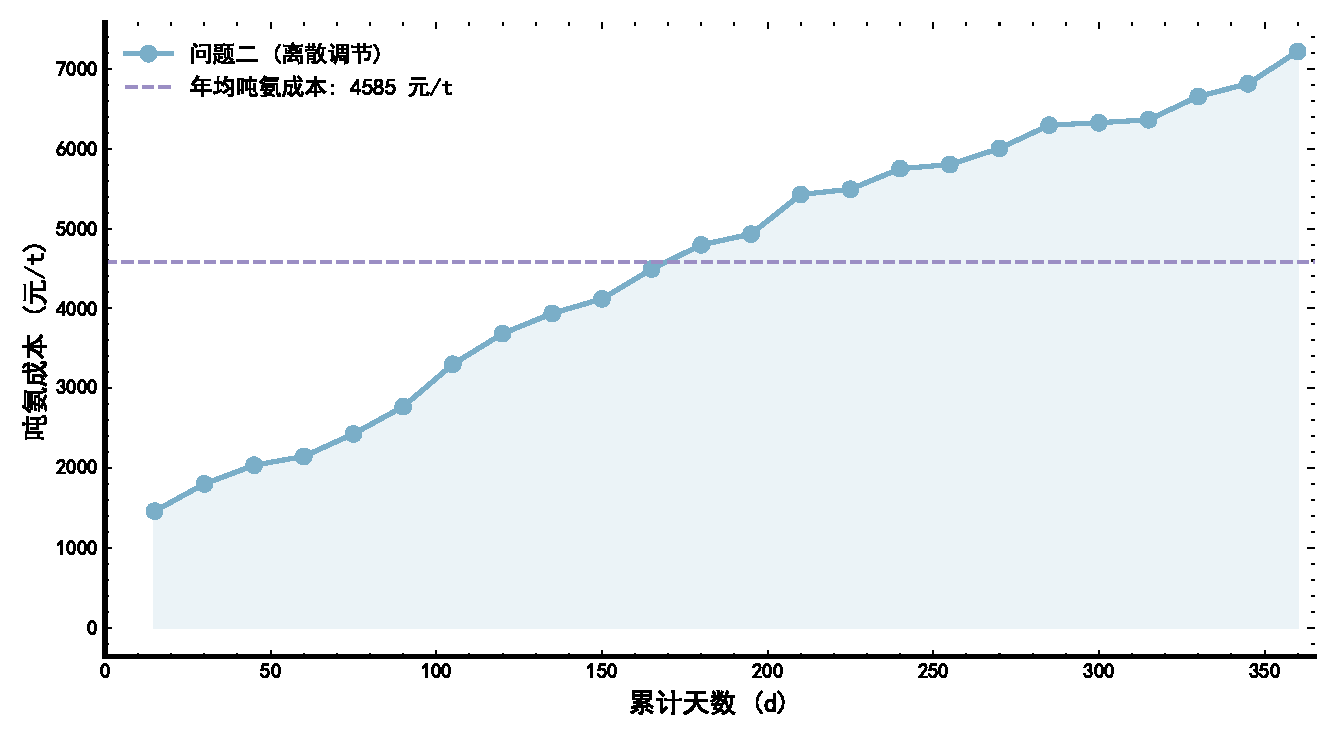
\includegraphics[width=0.85\textwidth]{figures/fig_q2_annual_cost.pdf}
\caption{全年吨氨成本分布曲线（问题二，离散调节，36 t/d）}
\label{fig:q2_annual_cost}
\end{figure}

\begin{figure}[H]
\centering
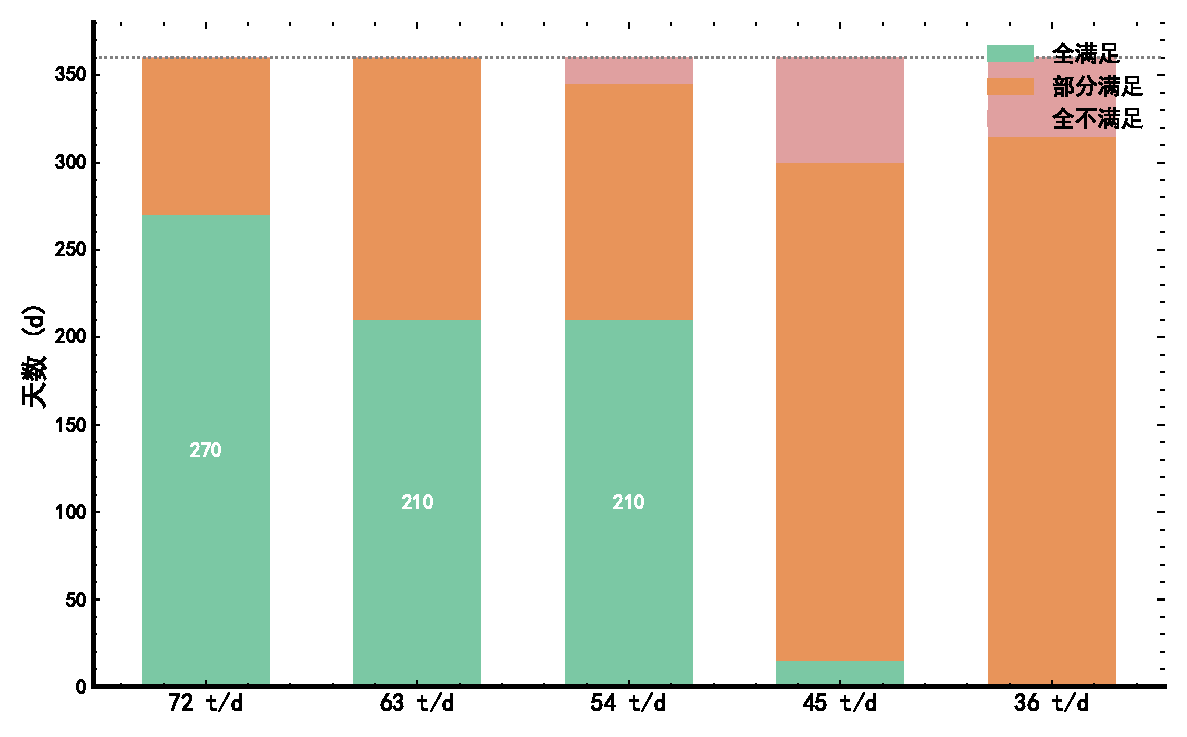
\includegraphics[width=0.78\textwidth]{figures/fig_q2_indicator_stats.pdf}
\caption{全年绿电直连指标满足情况统计}
\label{fig:q2_indicator_stats}
\end{figure}

% ==================== 问题三 ====================

\begin{figure}[H]
\centering
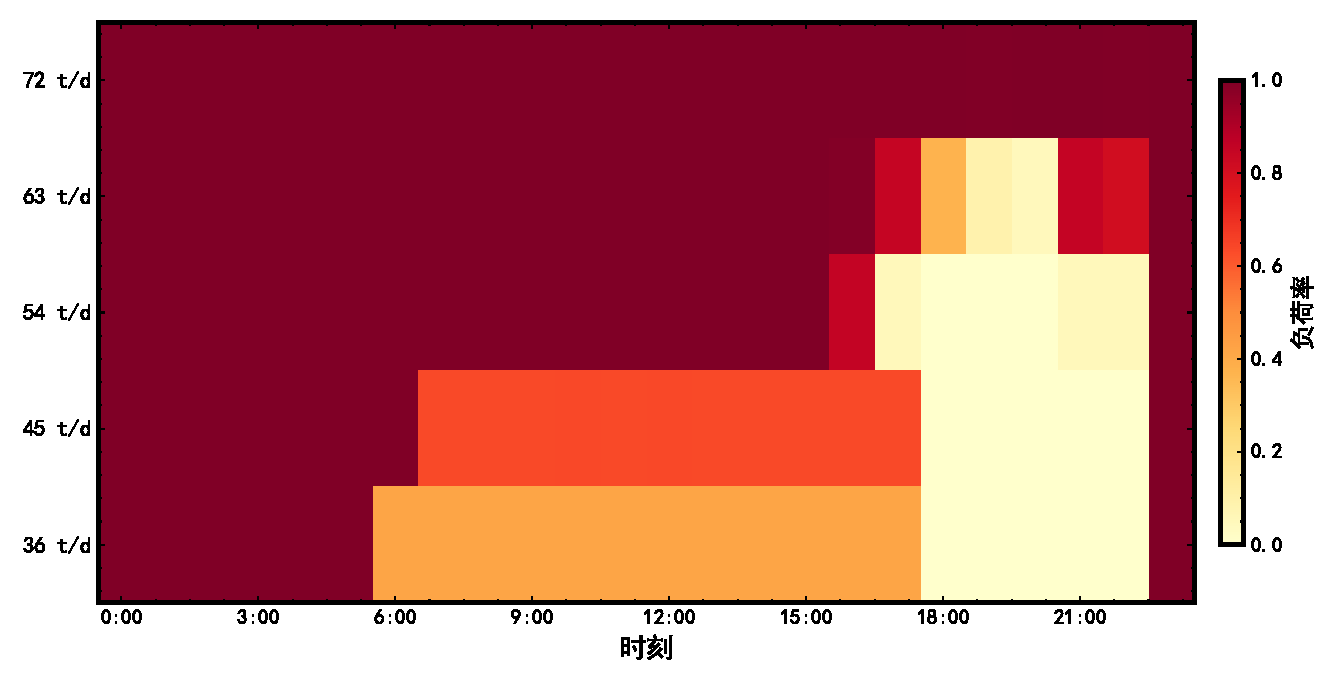
\includegraphics[width=0.92\textwidth]{figures/fig_q3_dispatch.pdf}
\caption{连续调节模式下各产量典型场景负荷率调度热力图}
\label{fig:q3_dispatch}
\end{figure}

\begin{figure}[H]
\centering
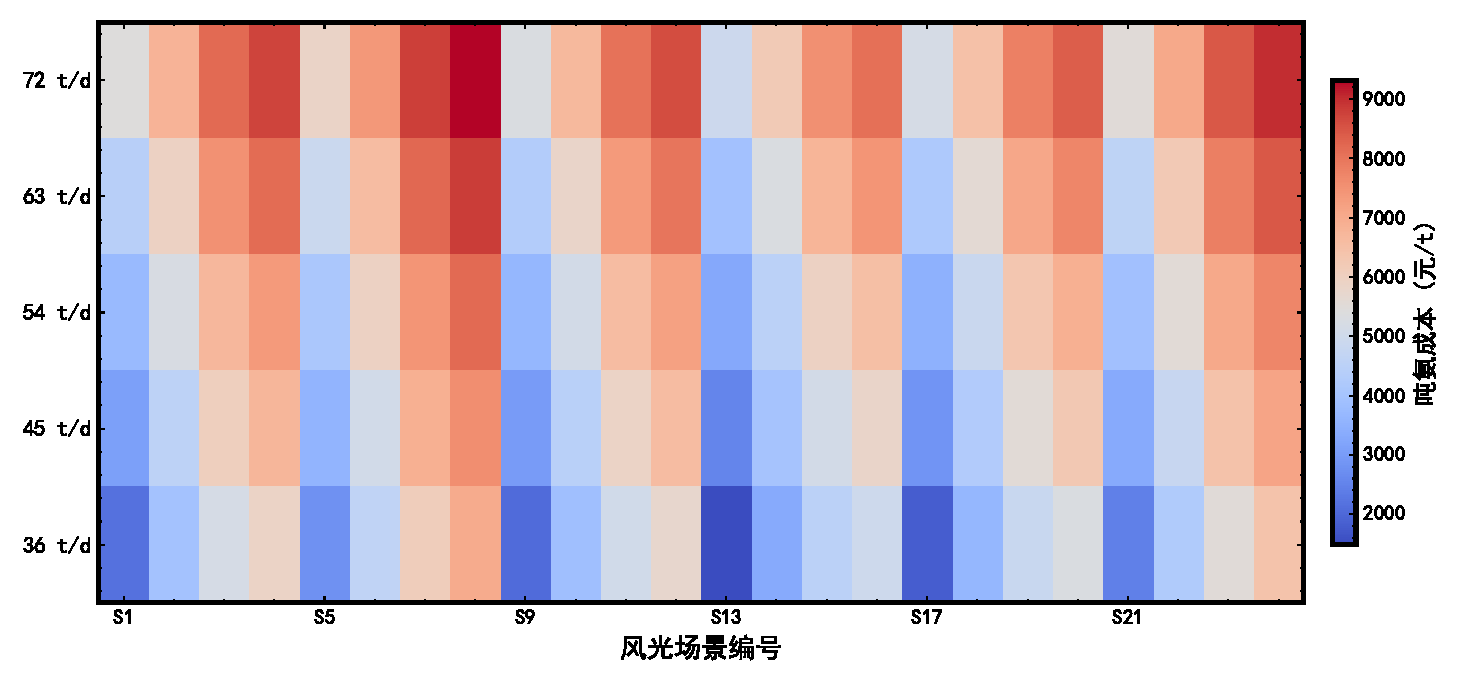
\includegraphics[width=0.92\textwidth]{figures/fig_q3_alpha_heatmap.pdf}
\caption{24种场景下各产量吨氨成本热力图}
\label{fig:q3_alpha_heatmap}
\end{figure}

\begin{figure}[H]
\centering
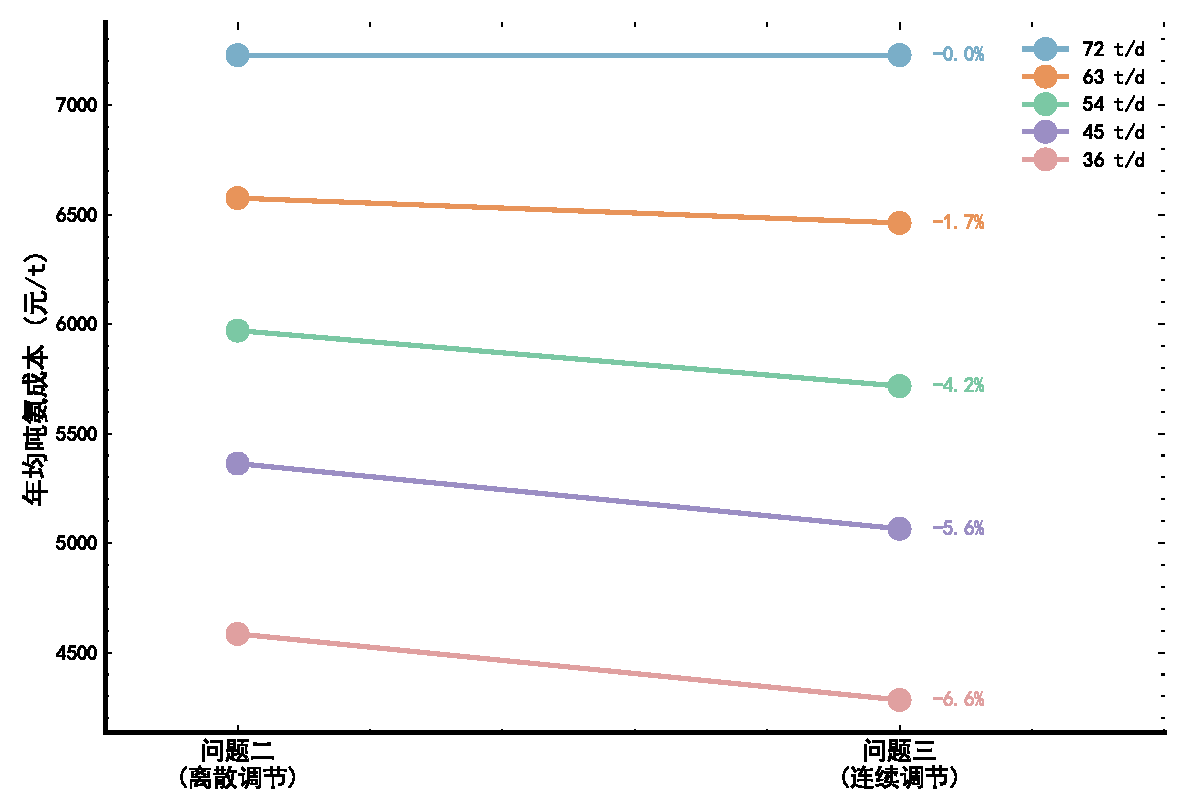
\includegraphics[width=0.78\textwidth]{figures/fig_q3_compare_q2.pdf}
\caption{问题三与问题二年均吨氨成本配对对比图}
\label{fig:q3_compare_q2}
\end{figure}

\begin{figure}[H]
\centering
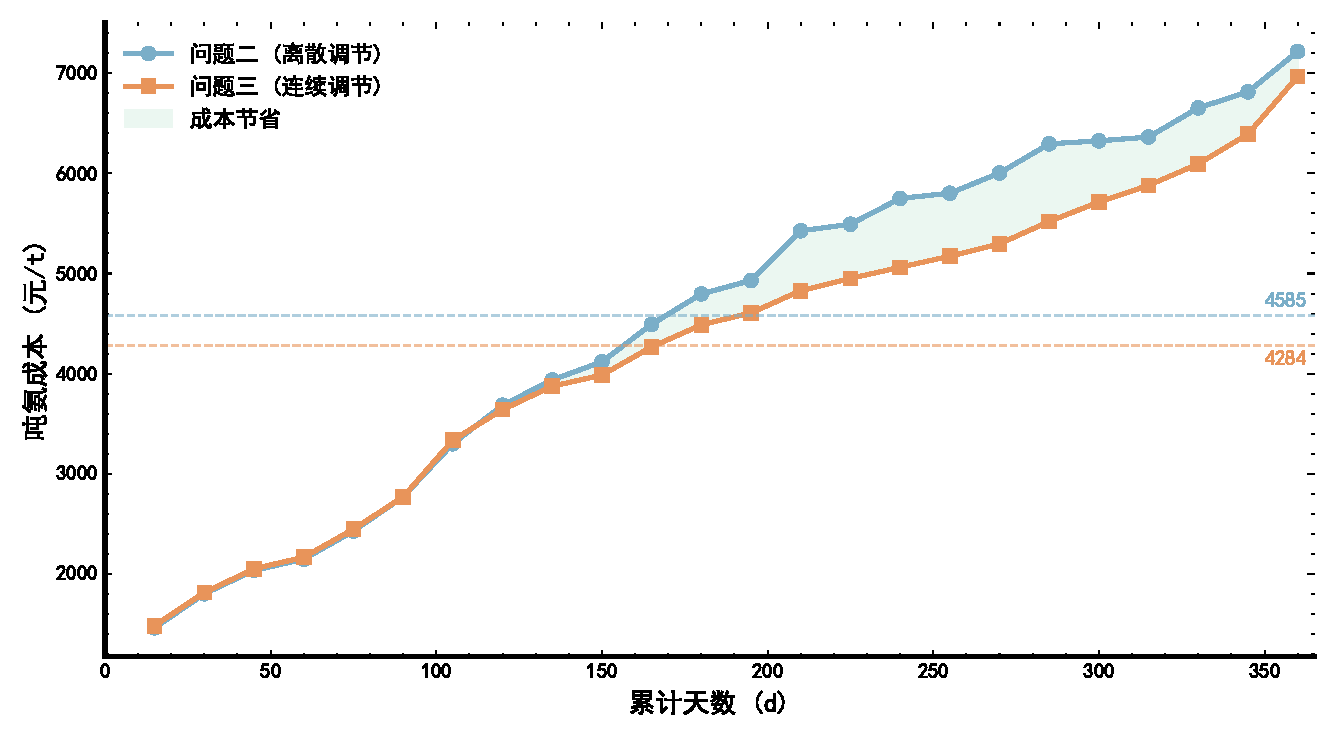
\includegraphics[width=0.85\textwidth]{figures/fig_q3_annual_cost.pdf}
\caption{全年吨氨成本分布曲线（问题二与问题三对比）}
\label{fig:q3_annual_cost}
\end{figure}

% ==================== 问题四 ====================

\begin{figure}[H]
\centering
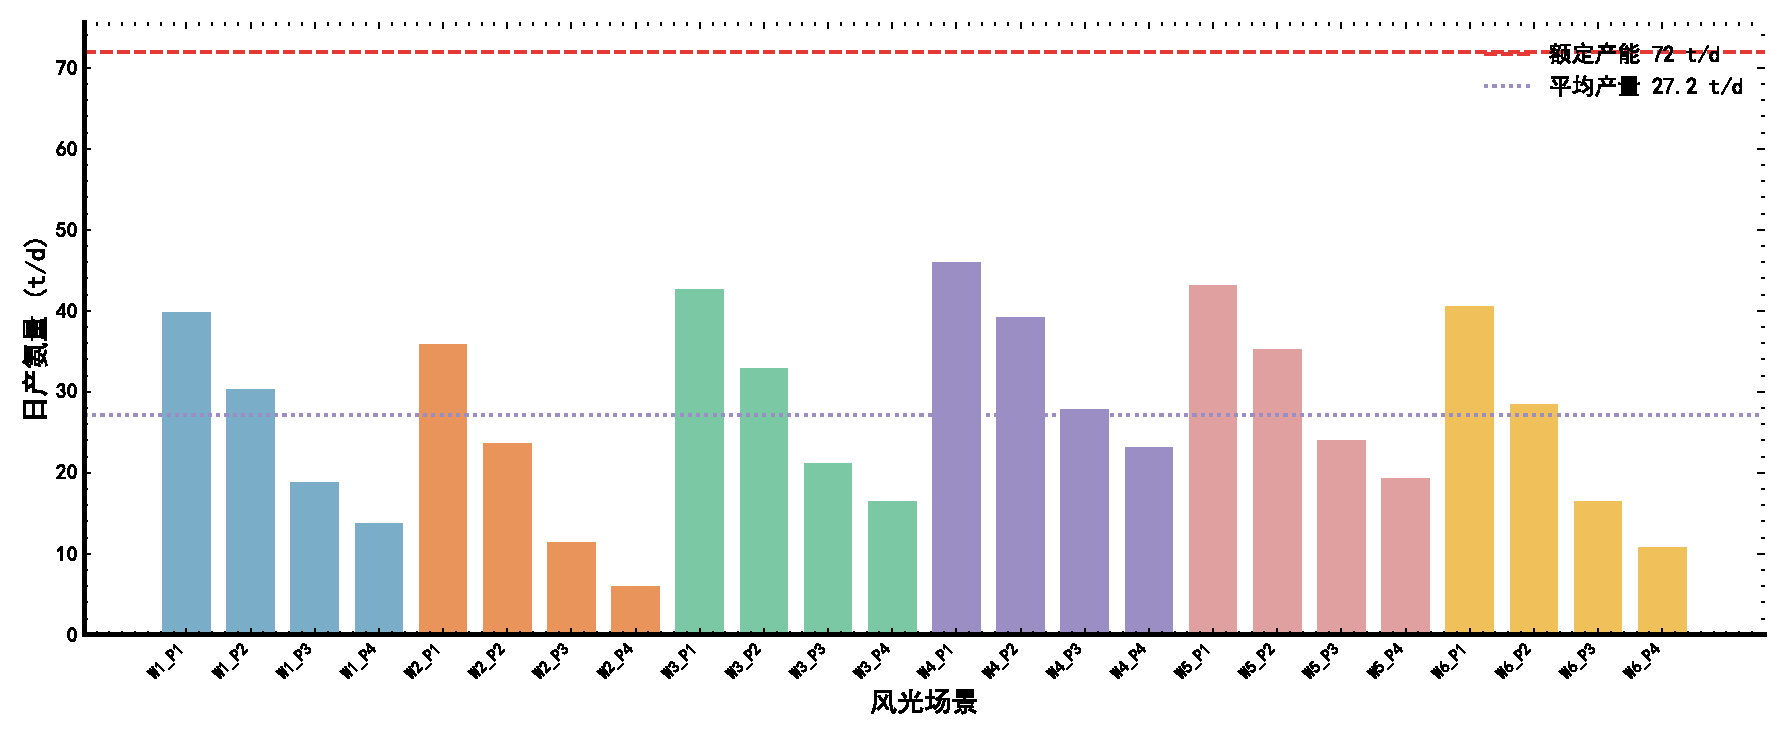
\includegraphics[width=0.95\textwidth]{figures/fig_q4_offgrid_production.pdf}
\caption{24种风光场景下离网运行日产氨量}
\label{fig:q4_offgrid_production}
\end{figure}

\begin{figure}[H]
\centering
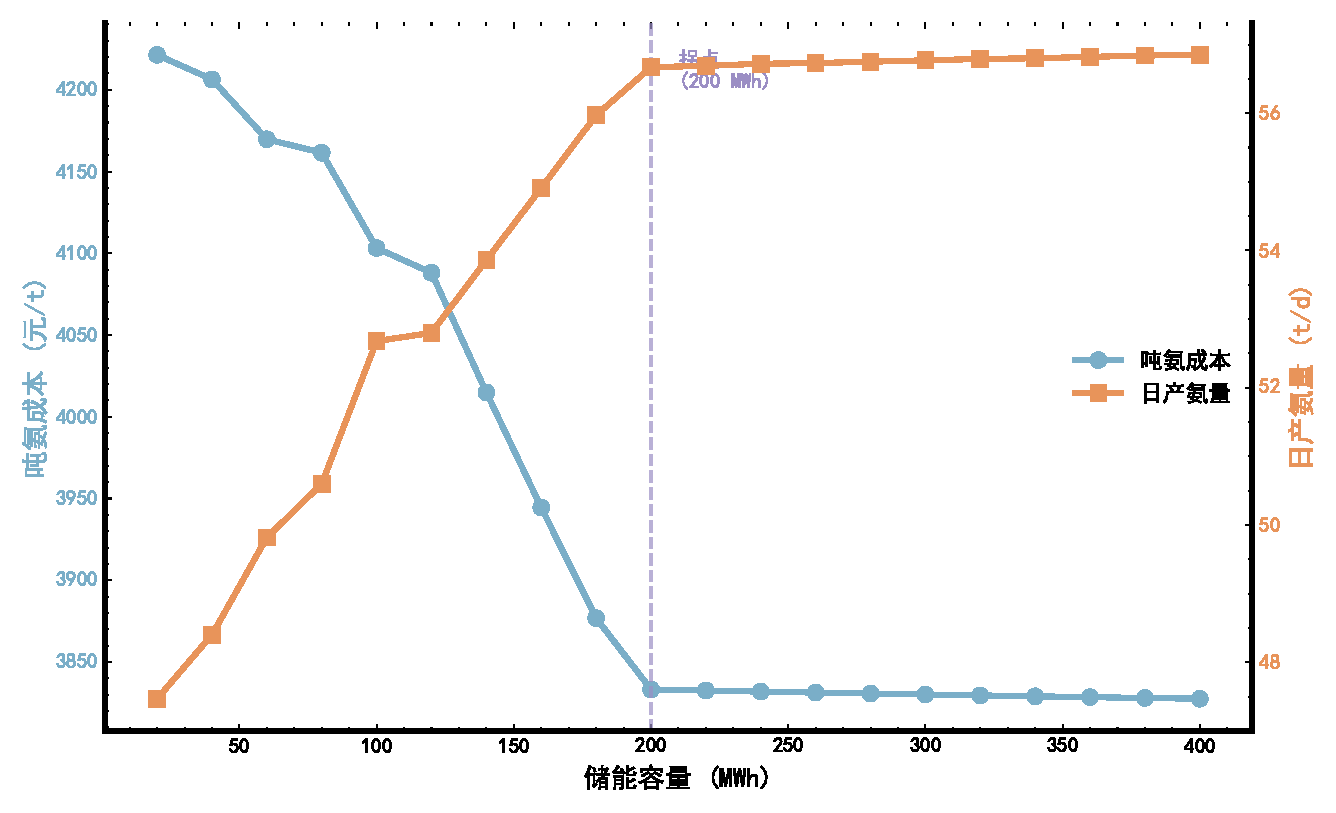
\includegraphics[width=0.82\textwidth]{figures/fig_q4_storage_optimization.pdf}
\caption{储能容量与吨氨成本、日产氨量关系曲线}
\label{fig:q4_storage_optimization}
\end{figure}

\begin{figure}[H]
\centering
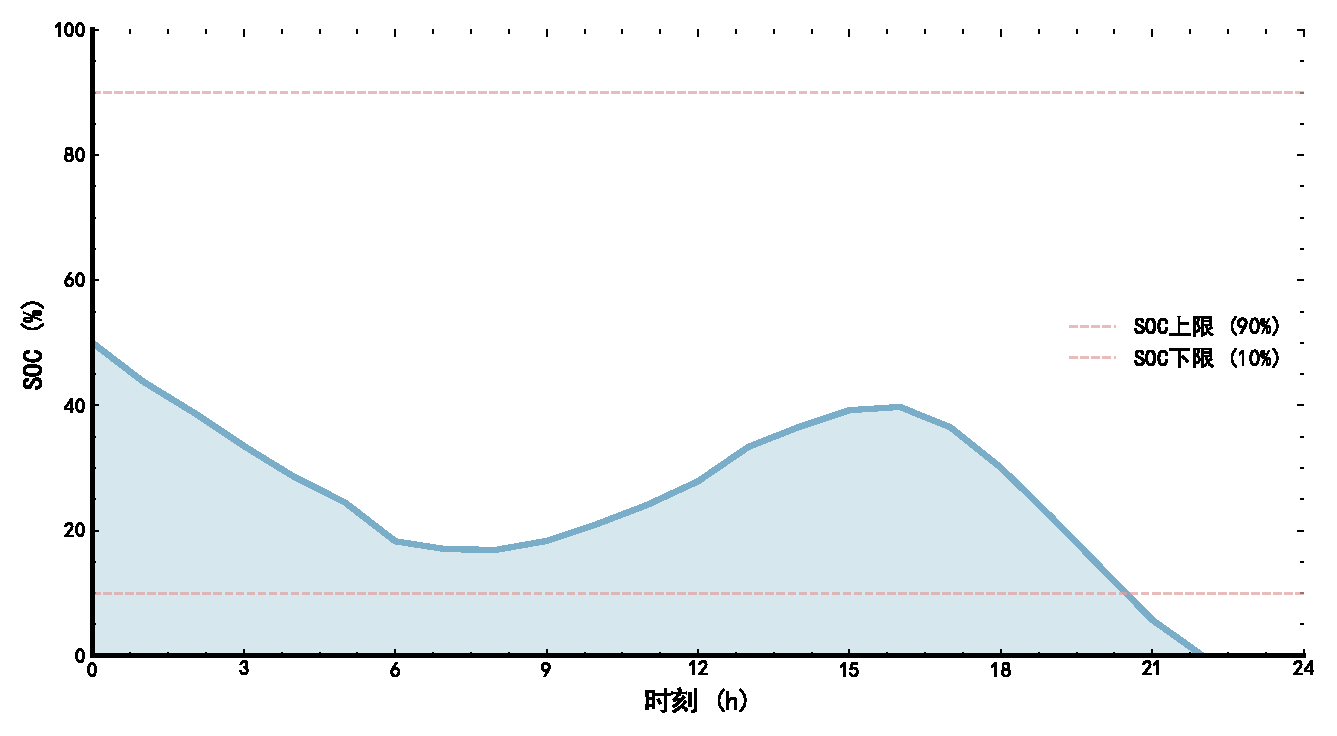
\includegraphics[width=0.82\textwidth]{figures/fig_q4_soc_curve.pdf}
\caption{最大弃电场景储能SOC变化曲线}
\label{fig:q4_soc_curve}
\end{figure}

\begin{figure}[H]
\centering
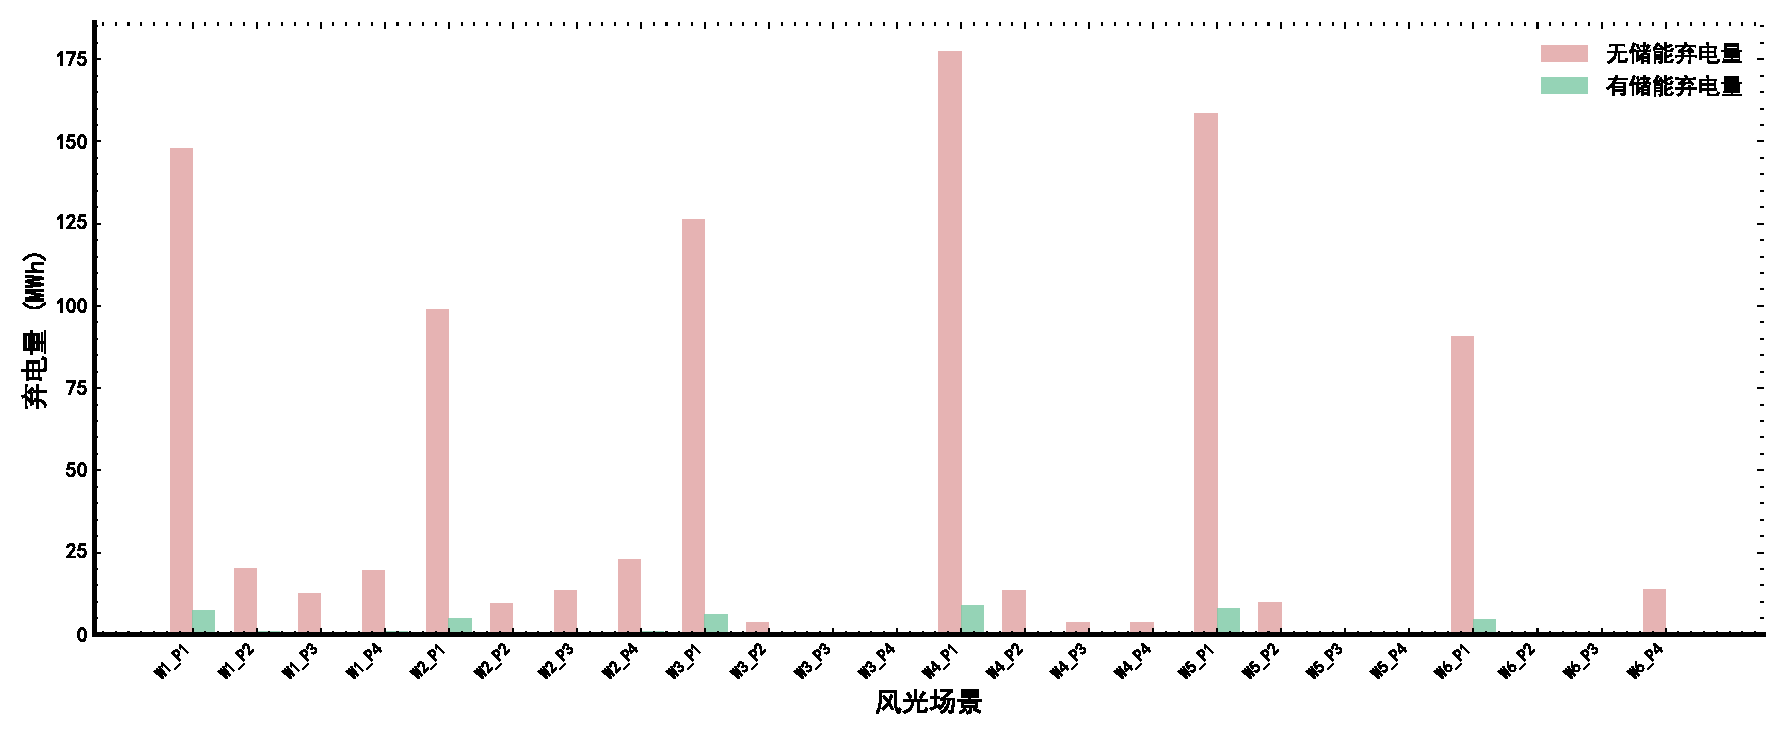
\includegraphics[width=0.95\textwidth]{figures/fig_q4_curtail_compare.pdf}
\caption{有无储能弃电量对比}
\label{fig:q4_curtail_compare}
\end{figure}

\begin{figure}[H]
\centering
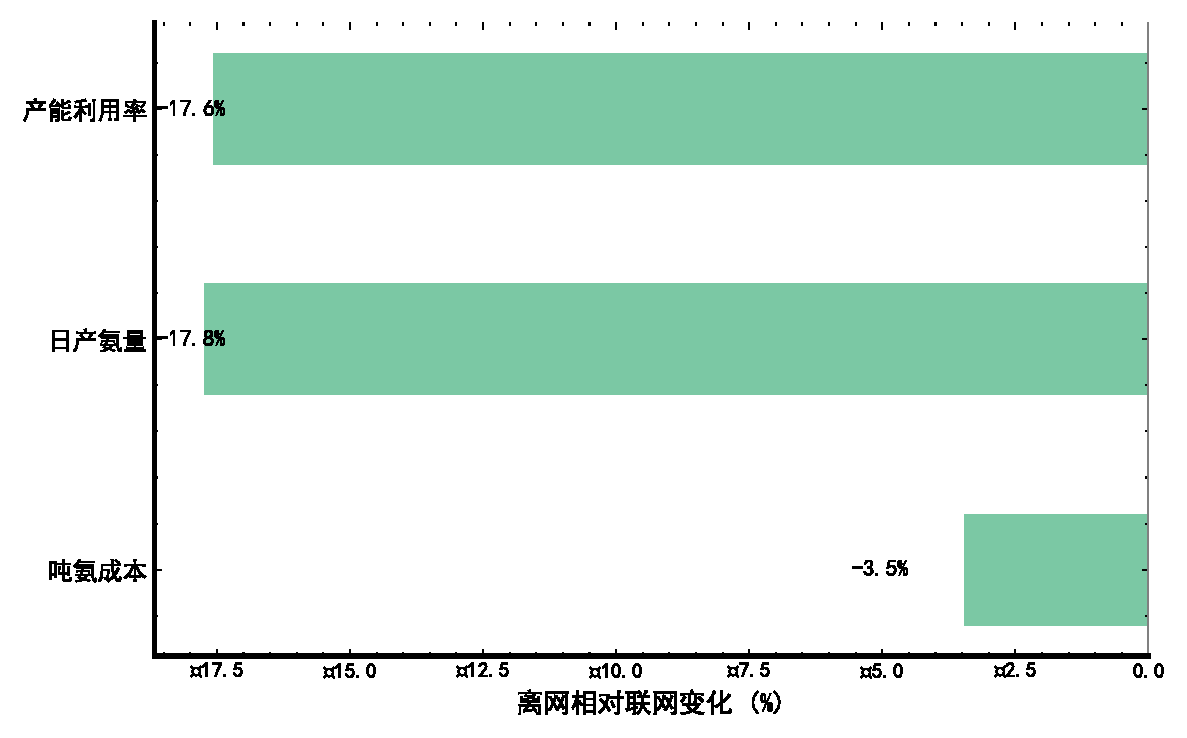
\includegraphics[width=0.75\textwidth]{figures/fig_q4_onoff_compare.pdf}
\caption{离网与联网运行模式经济性对比（发散柱状图）}
\label{fig:q4_onoff_compare}
\end{figure}

% ==================== 灵敏度分析 ====================

\begin{figure}[H]
\centering
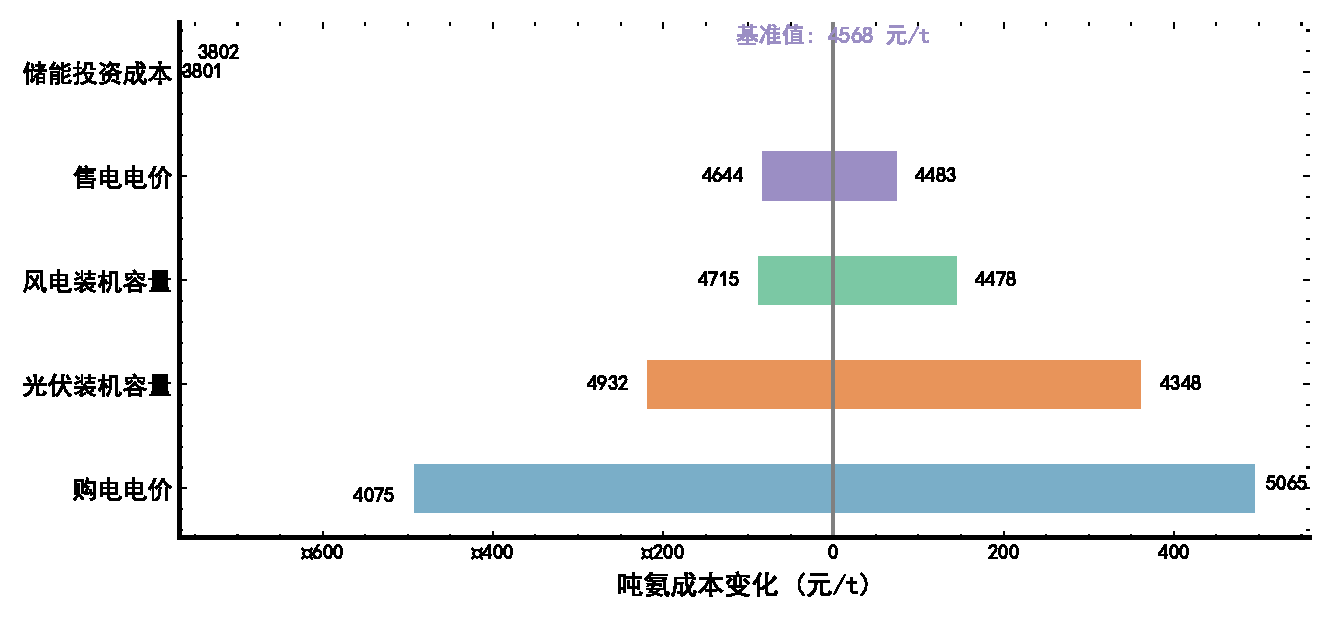
\includegraphics[width=0.82\textwidth]{figures/fig_sensitivity.pdf}
\caption{关键参数敏感性分析龙卷风图}
\label{fig:sensitivity}
\end{figure}

% ============================================================

% ==================== 技术路线图 ====================

\begin{figure}[H]
\centering
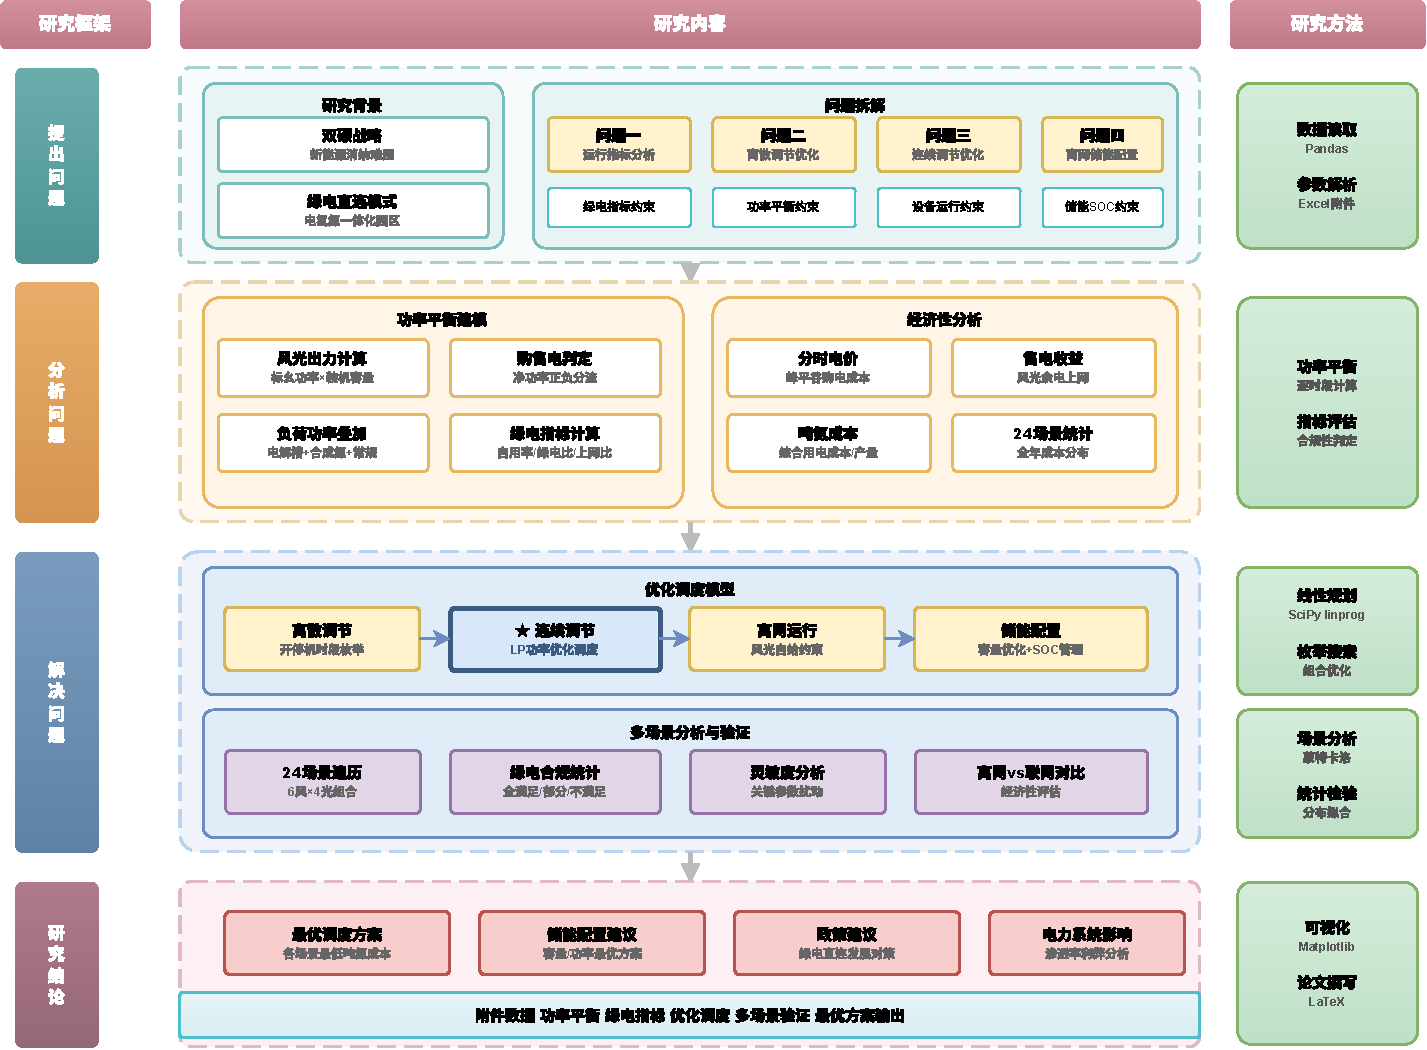
\includegraphics[width=\textwidth,height=0.45\textheight,keepaspectratio]{figures/fig_roadmap.pdf}
\caption{整体技术路线图}\label{fig:roadmap}
\end{figure}

% ==================== 园区系统架构图 ====================

\begin{figure}[H]
\centering
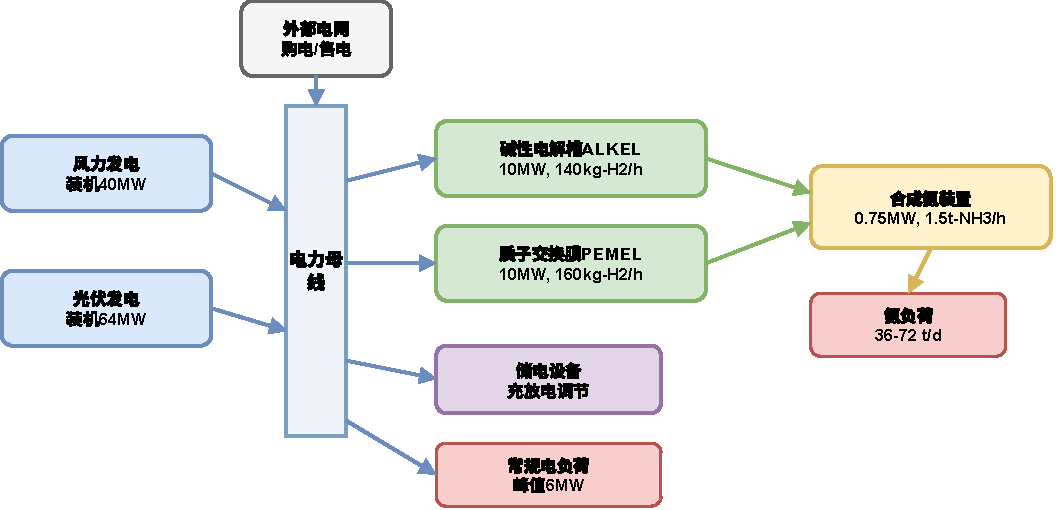
\includegraphics[width=0.9\textwidth,height=0.3\textheight,keepaspectratio]{figures/fig_system_arch.pdf}
\caption{绿电直连型电氢氨园区系统架构}\label{fig:system_arch}
\end{figure}

% ==================== 求解流程图 ====================

\begin{figure}[H]
\centering
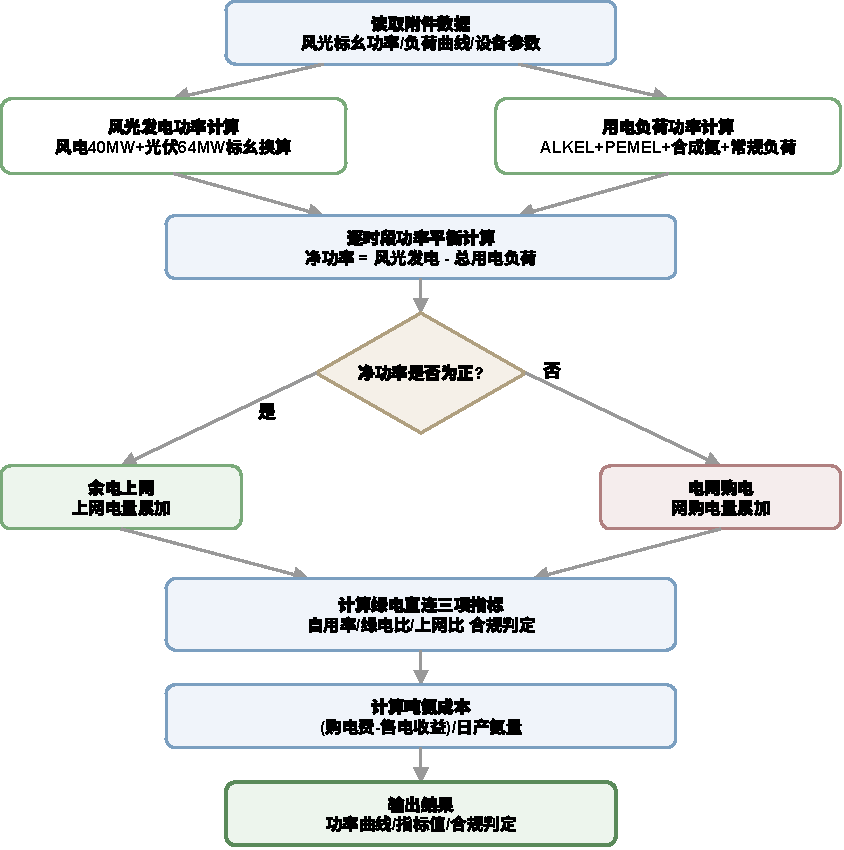
\includegraphics[width=0.85\textwidth,height=0.38\textheight,keepaspectratio]{figures/fig_flow_q1.pdf}
\caption{问题一求解流程图}\label{fig:flow_q1}
\end{figure}

\begin{figure}[H]
\centering
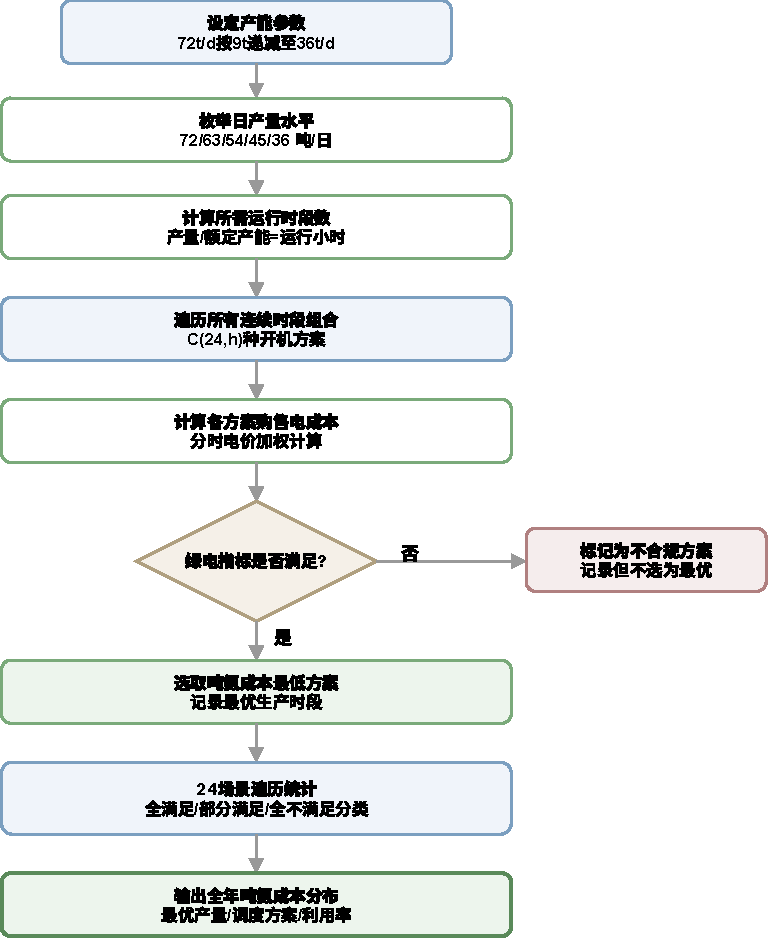
\includegraphics[width=0.85\textwidth,height=0.38\textheight,keepaspectratio]{figures/fig_flow_q2.pdf}
\caption{问题二求解流程图}\label{fig:flow_q2}
\end{figure}

\begin{figure}[H]
\centering
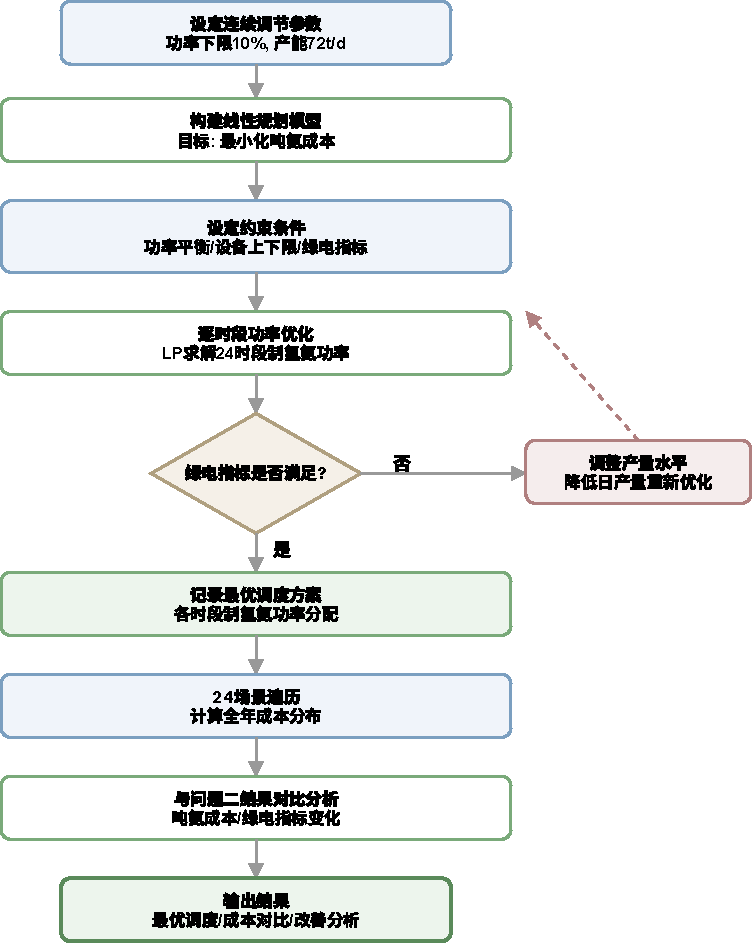
\includegraphics[width=0.85\textwidth,height=0.38\textheight,keepaspectratio]{figures/fig_flow_q3.pdf}
\caption{问题三求解流程图}\label{fig:flow_q3}
\end{figure}

\begin{figure}[H]
\centering
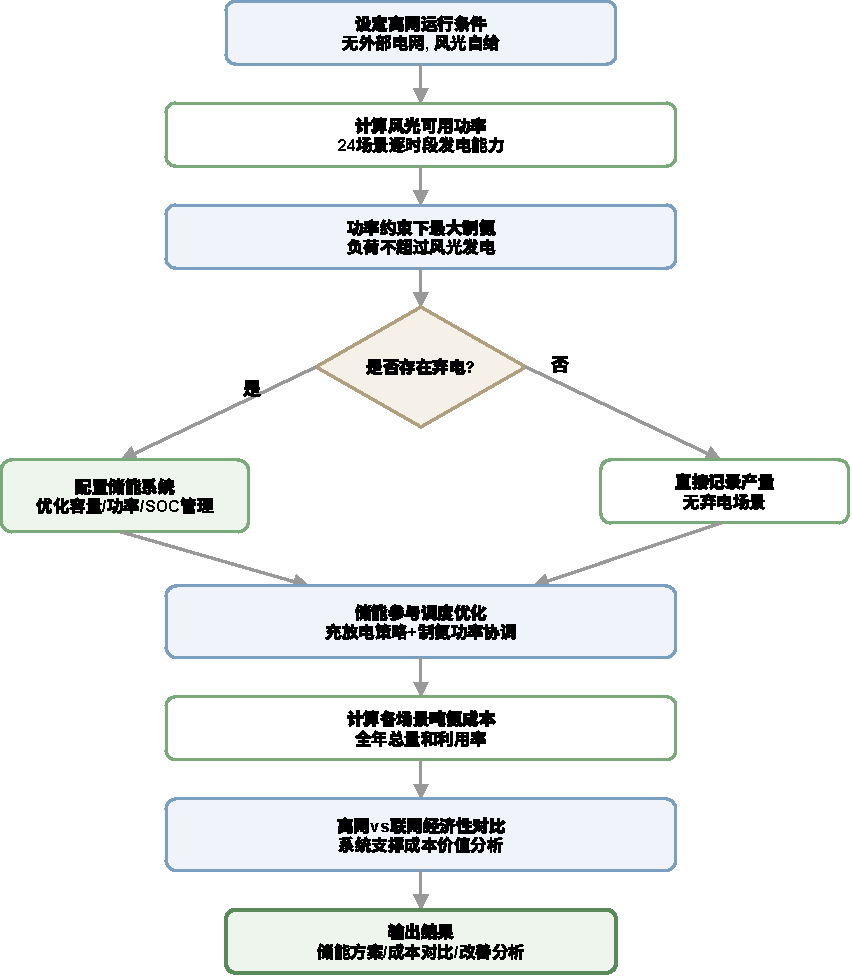
\includegraphics[width=0.85\textwidth,height=0.38\textheight,keepaspectratio]{figures/fig_flow_q4.pdf}
\caption{问题四求解流程图}\label{fig:flow_q4}
\end{figure}

% ==================== 问题一 ====================

\begin{figure}[H]
\centering
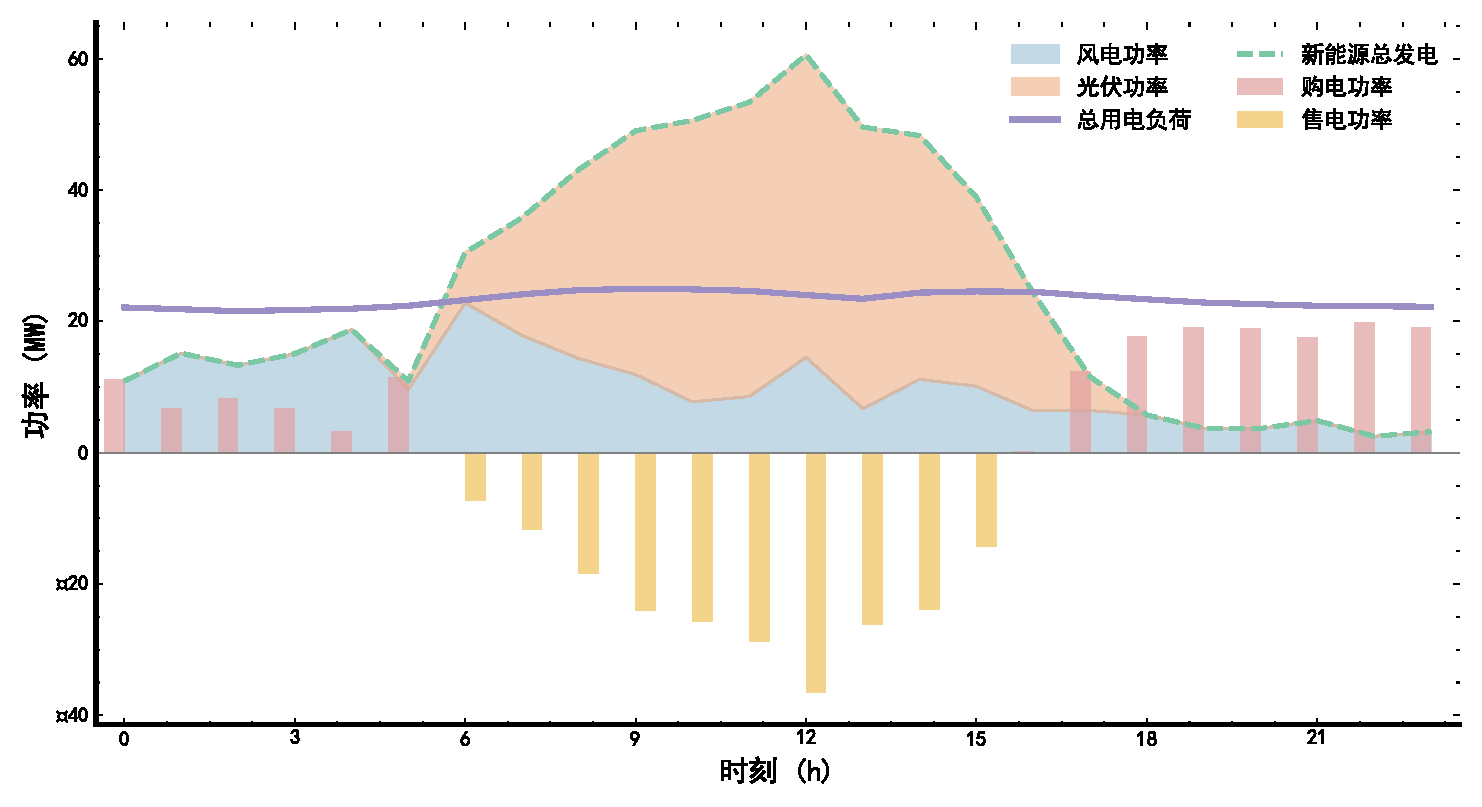
\includegraphics[width=0.95\textwidth]{figures/fig_q1_power_balance.pdf}
\caption{典型日功率平衡曲线（风电、光伏发电与负荷、购售电功率对比）}
\label{fig:q1_power_balance}
\end{figure}

\begin{figure}[H]
\centering
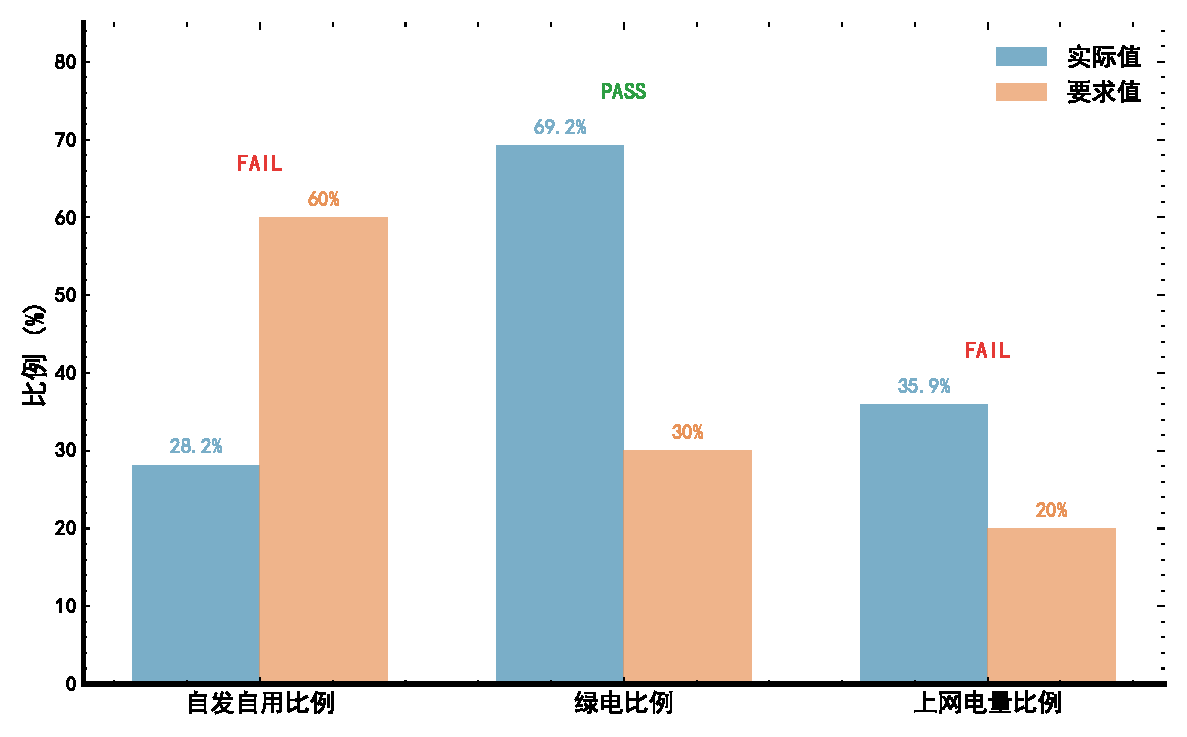
\includegraphics[width=0.75\textwidth]{figures/fig_q1_indicators.pdf}
\caption{绿电直连指标实际值与要求值对比}
\label{fig:q1_indicators}
\end{figure}

% ==================== 问题二 ====================

\begin{figure}[H]
\centering
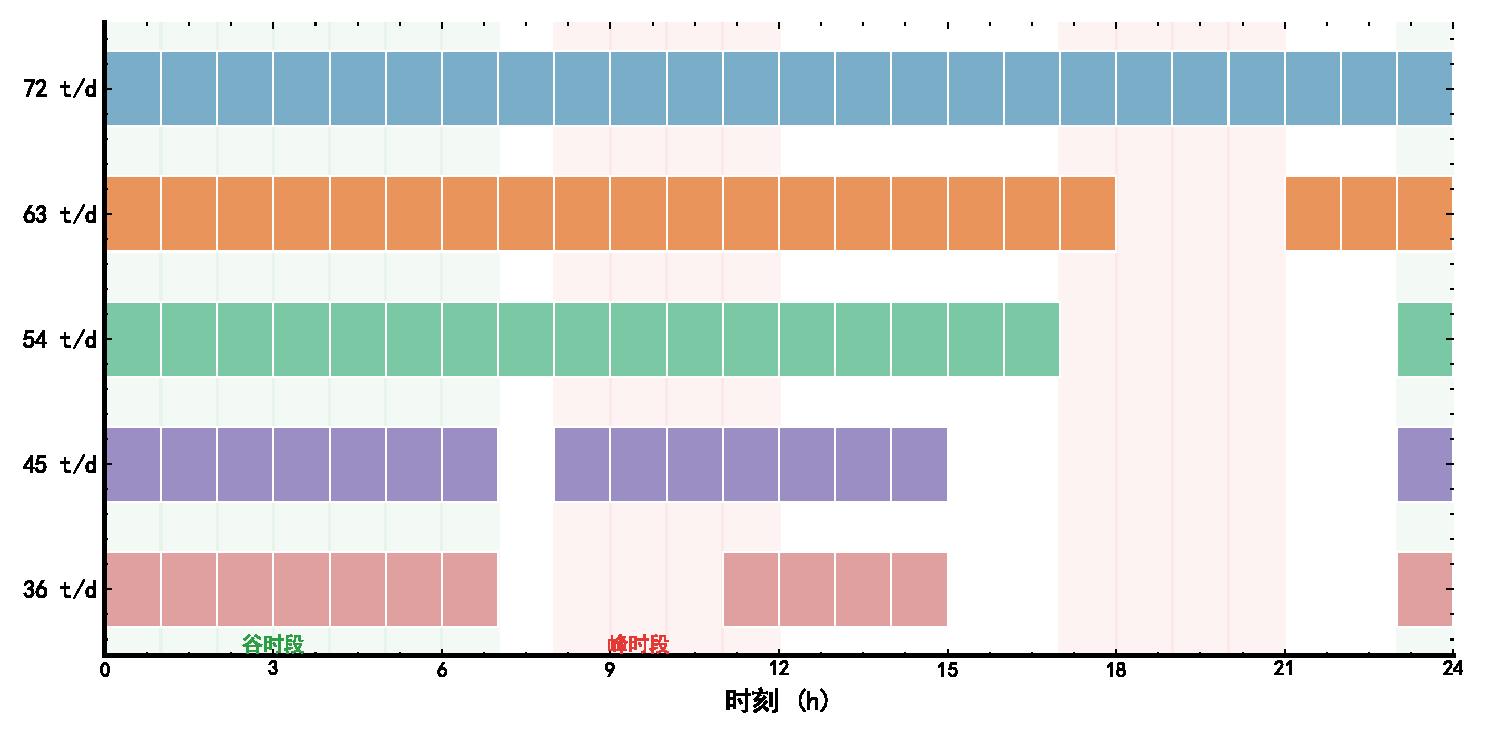
\includegraphics[width=0.92\textwidth]{figures/fig_q2_gantt.pdf}
\caption{不同产量下最优开机时段安排甘特图}
\label{fig:q2_gantt}
\end{figure}

\begin{figure}[H]
\centering
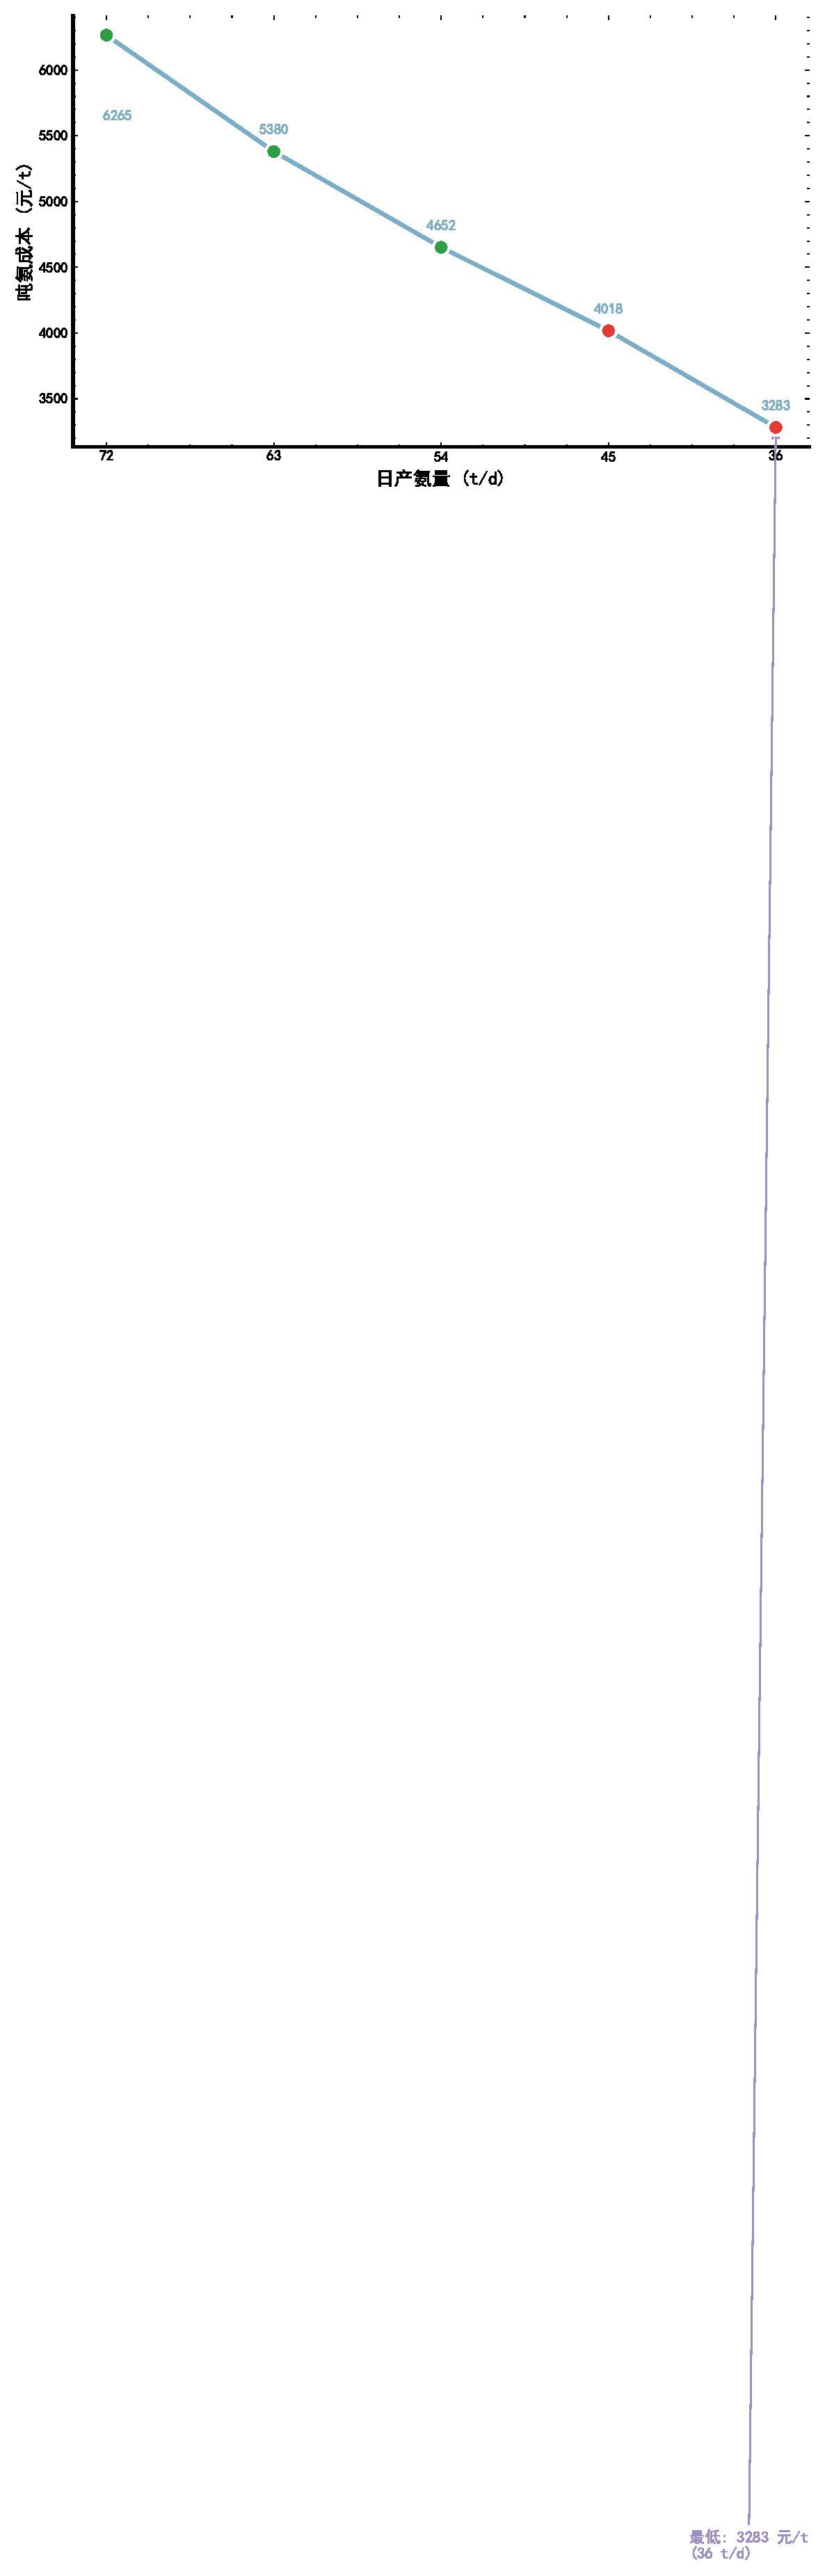
\includegraphics[width=0.78\textwidth]{figures/fig_q2_cost_vs_production.pdf}
\caption{吨氨成本随日产量变化曲线}
\label{fig:q2_cost_vs_production}
\end{figure}

\begin{figure}[H]
\centering
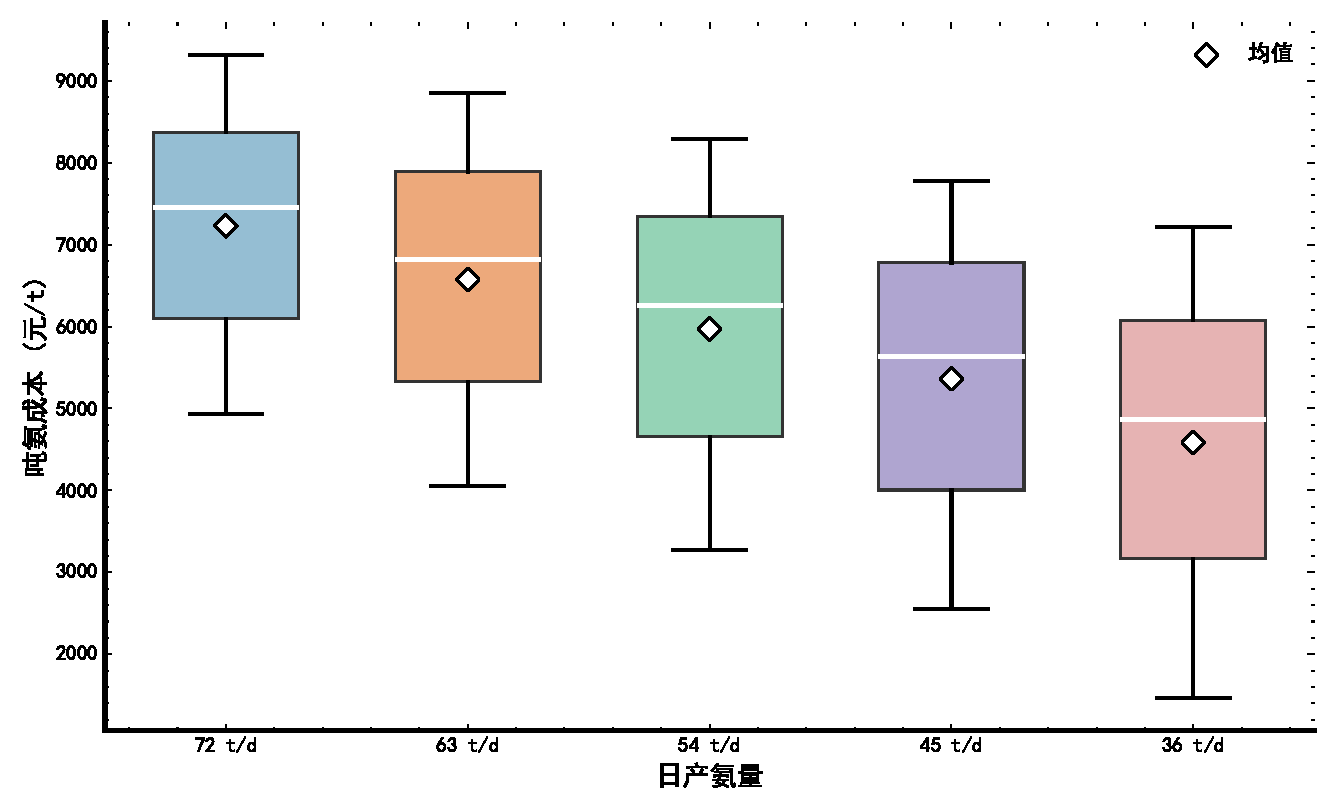
\includegraphics[width=0.82\textwidth]{figures/fig_q2_24scenes_cost.pdf}
\caption{24种风光场景下各产量吨氨成本分布箱线图}
\label{fig:q2_24scenes_cost}
\end{figure}

\begin{figure}[H]
\centering
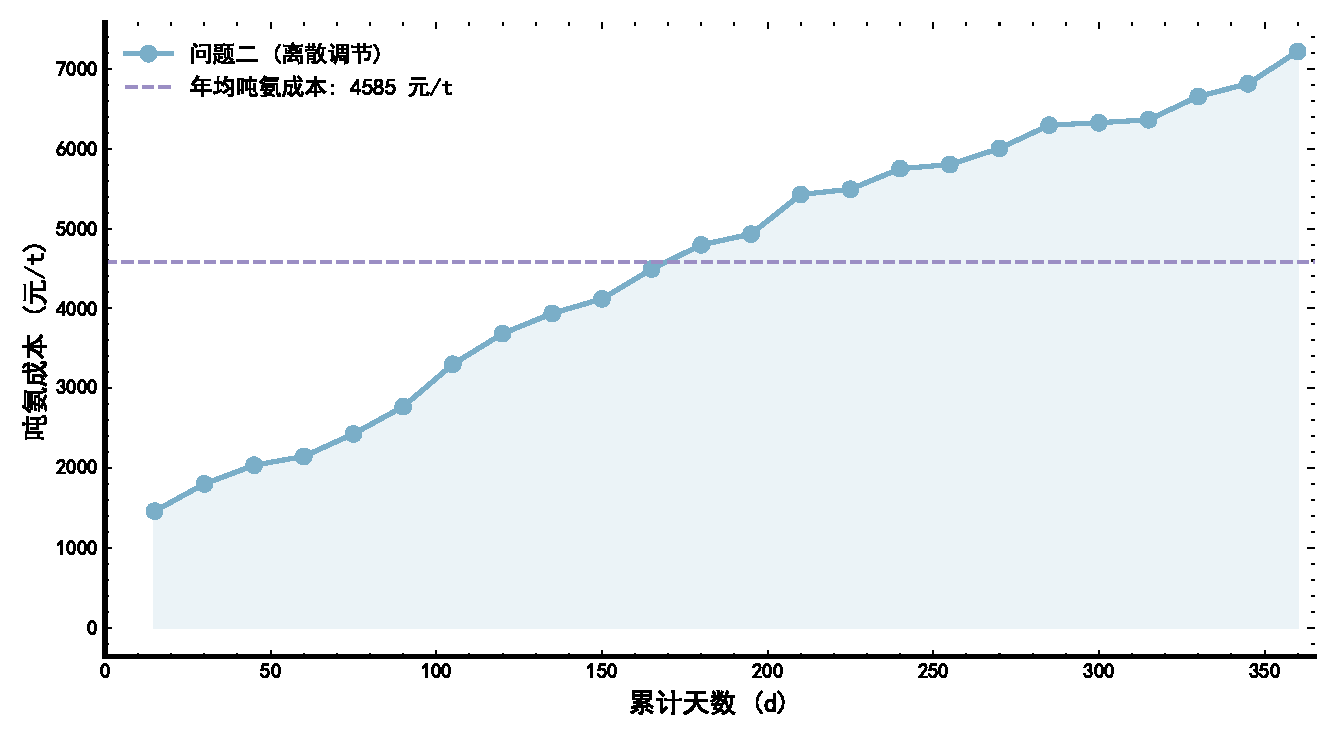
\includegraphics[width=0.85\textwidth]{figures/fig_q2_annual_cost.pdf}
\caption{全年吨氨成本分布曲线（问题二，离散调节，36 t/d）}
\label{fig:q2_annual_cost}
\end{figure}

\begin{figure}[H]
\centering
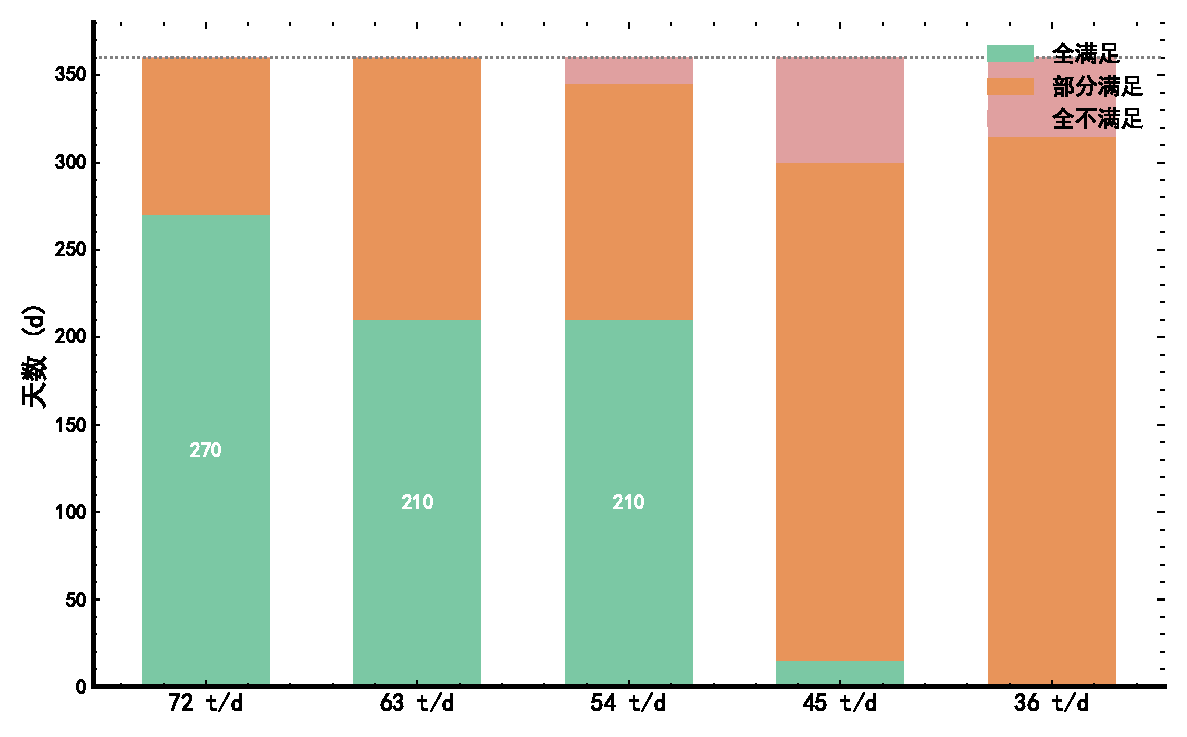
\includegraphics[width=0.78\textwidth]{figures/fig_q2_indicator_stats.pdf}
\caption{全年绿电直连指标满足情况统计}
\label{fig:q2_indicator_stats}
\end{figure}

% ==================== 问题三 ====================

\begin{figure}[H]
\centering
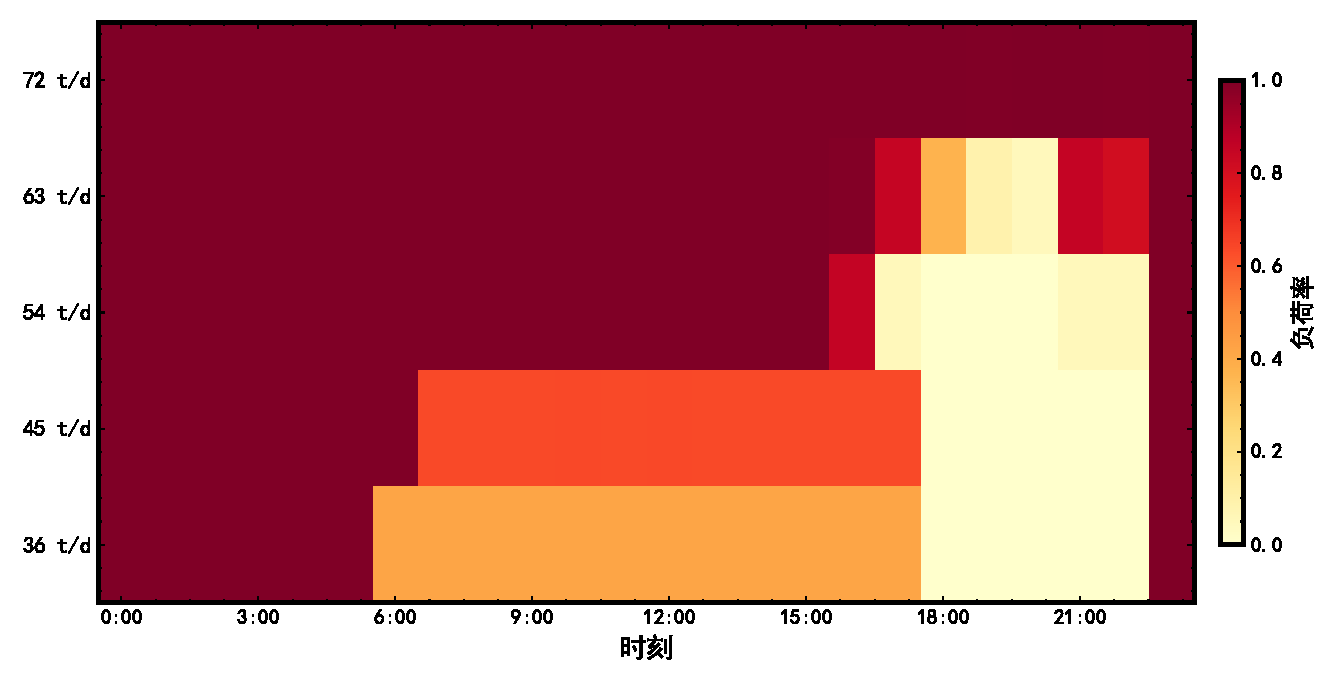
\includegraphics[width=0.92\textwidth]{figures/fig_q3_dispatch.pdf}
\caption{连续调节模式下各产量典型场景负荷率调度热力图}
\label{fig:q3_dispatch}
\end{figure}

\begin{figure}[H]
\centering
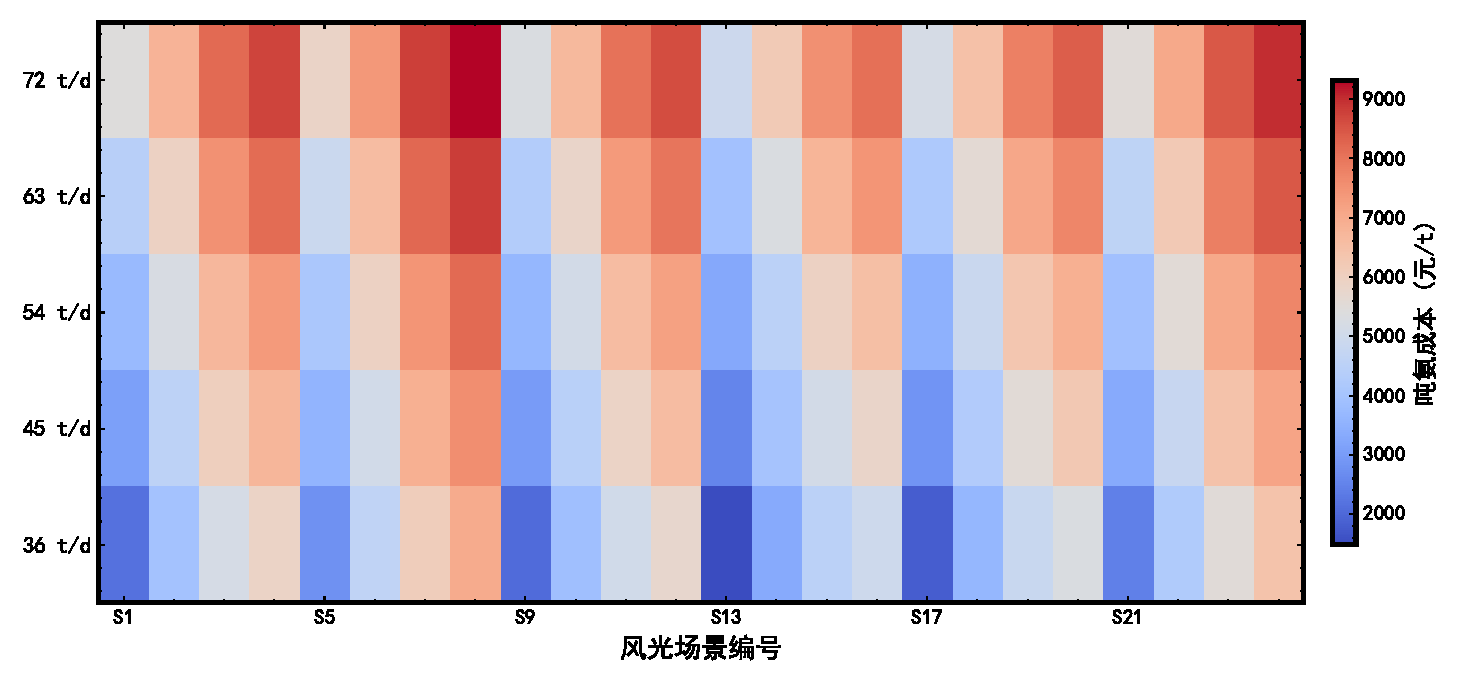
\includegraphics[width=0.92\textwidth]{figures/fig_q3_alpha_heatmap.pdf}
\caption{24种场景下各产量吨氨成本热力图}
\label{fig:q3_alpha_heatmap}
\end{figure}

\begin{figure}[H]
\centering
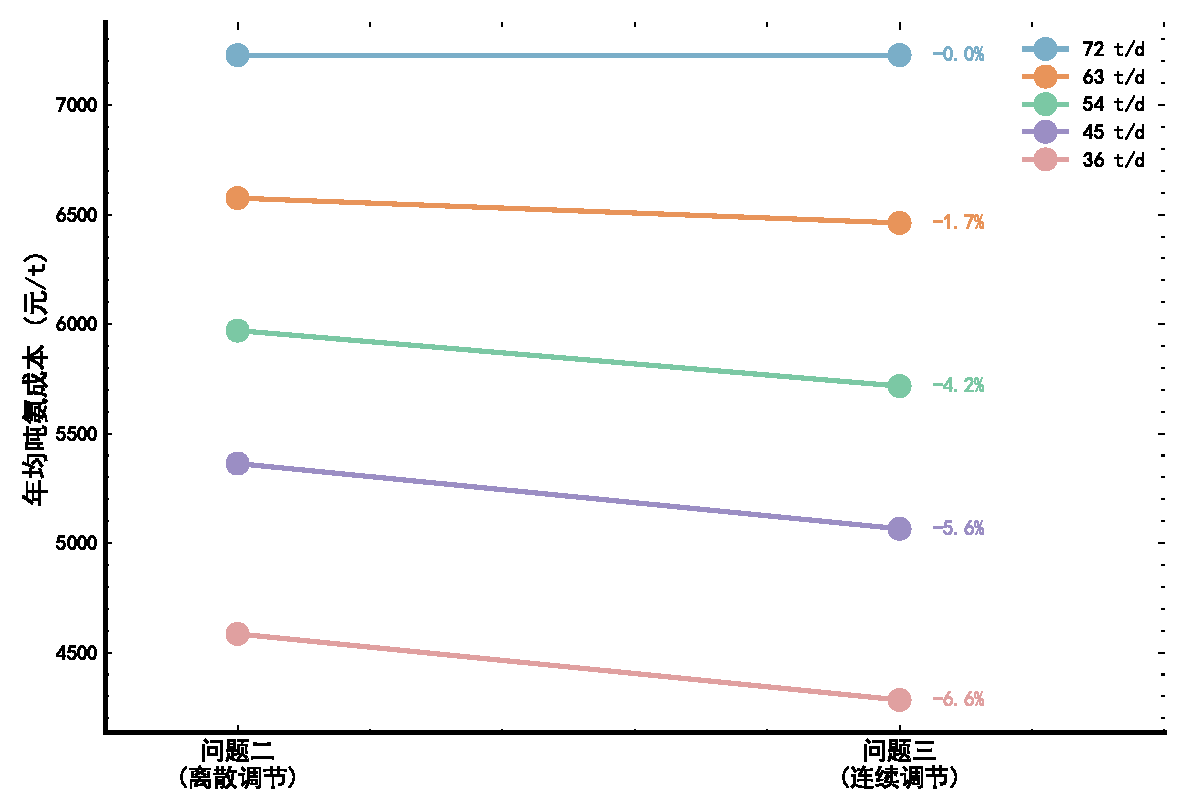
\includegraphics[width=0.78\textwidth]{figures/fig_q3_compare_q2.pdf}
\caption{问题三与问题二年均吨氨成本配对对比图}
\label{fig:q3_compare_q2}
\end{figure}

\begin{figure}[H]
\centering
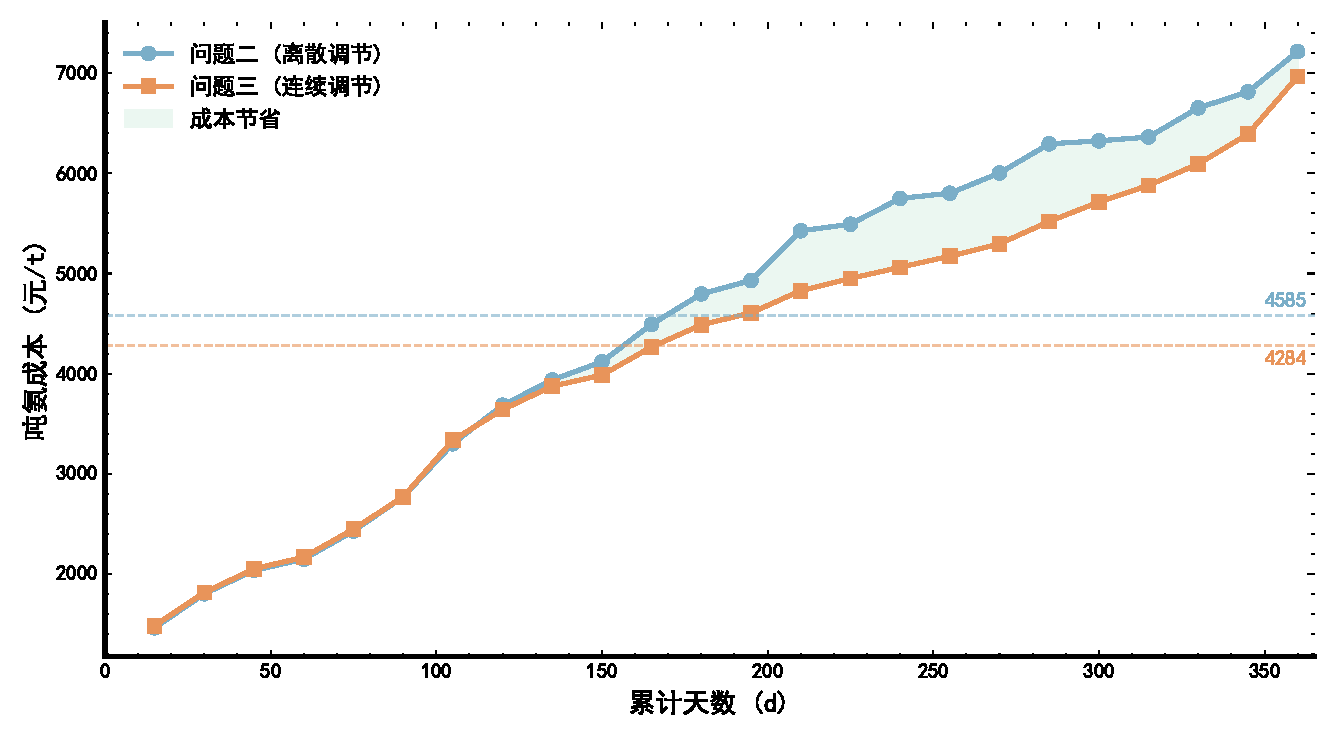
\includegraphics[width=0.85\textwidth]{figures/fig_q3_annual_cost.pdf}
\caption{全年吨氨成本分布曲线（问题二与问题三对比）}
\label{fig:q3_annual_cost}
\end{figure}

% ==================== 问题四 ====================

\begin{figure}[H]
\centering
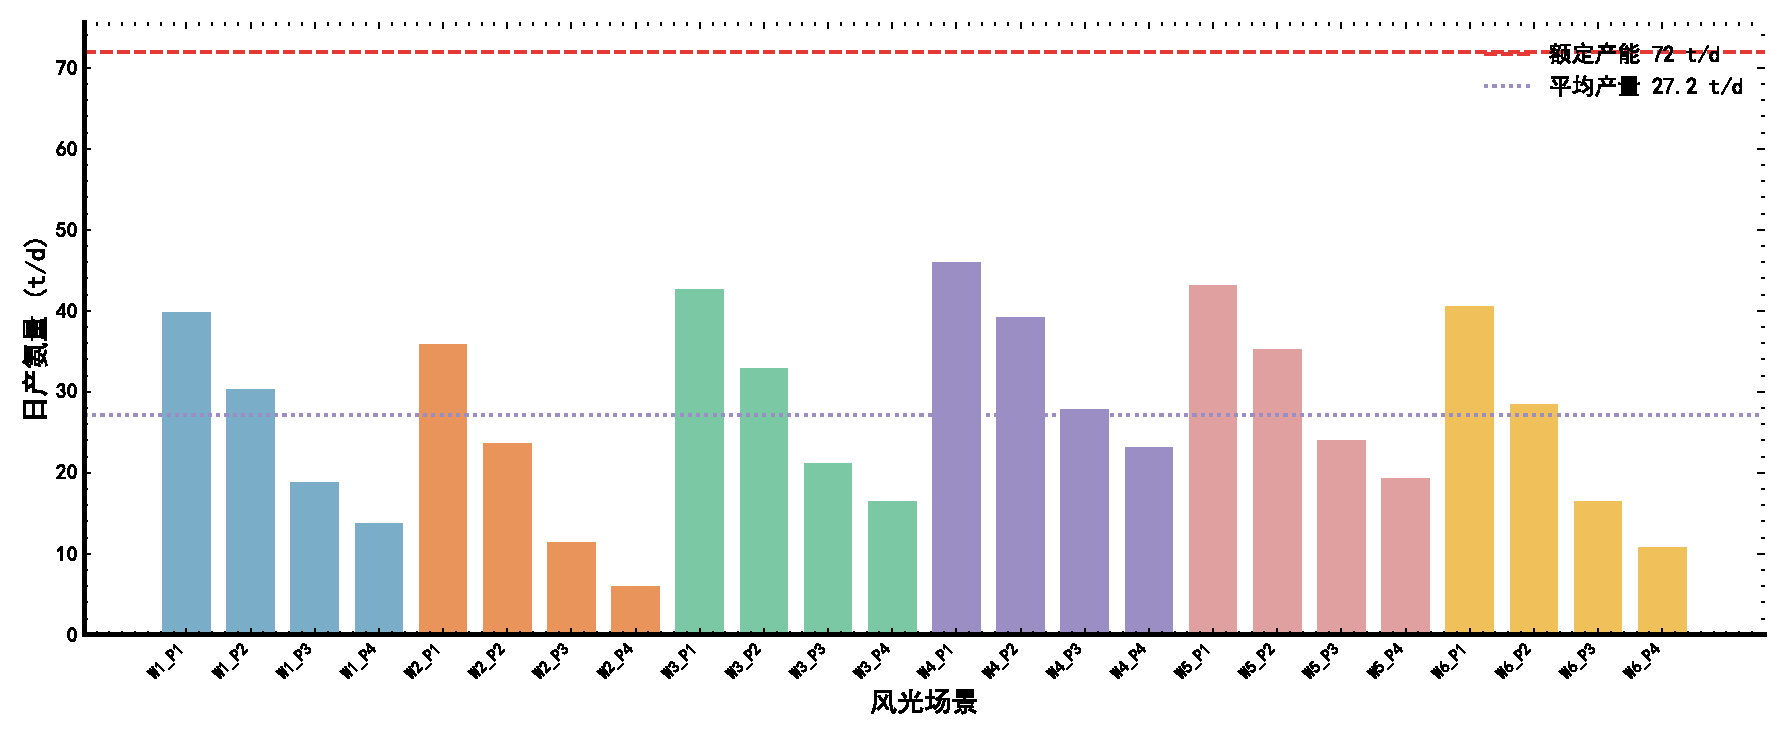
\includegraphics[width=0.95\textwidth]{figures/fig_q4_offgrid_production.pdf}
\caption{24种风光场景下离网运行日产氨量}
\label{fig:q4_offgrid_production}
\end{figure}

\begin{figure}[H]
\centering
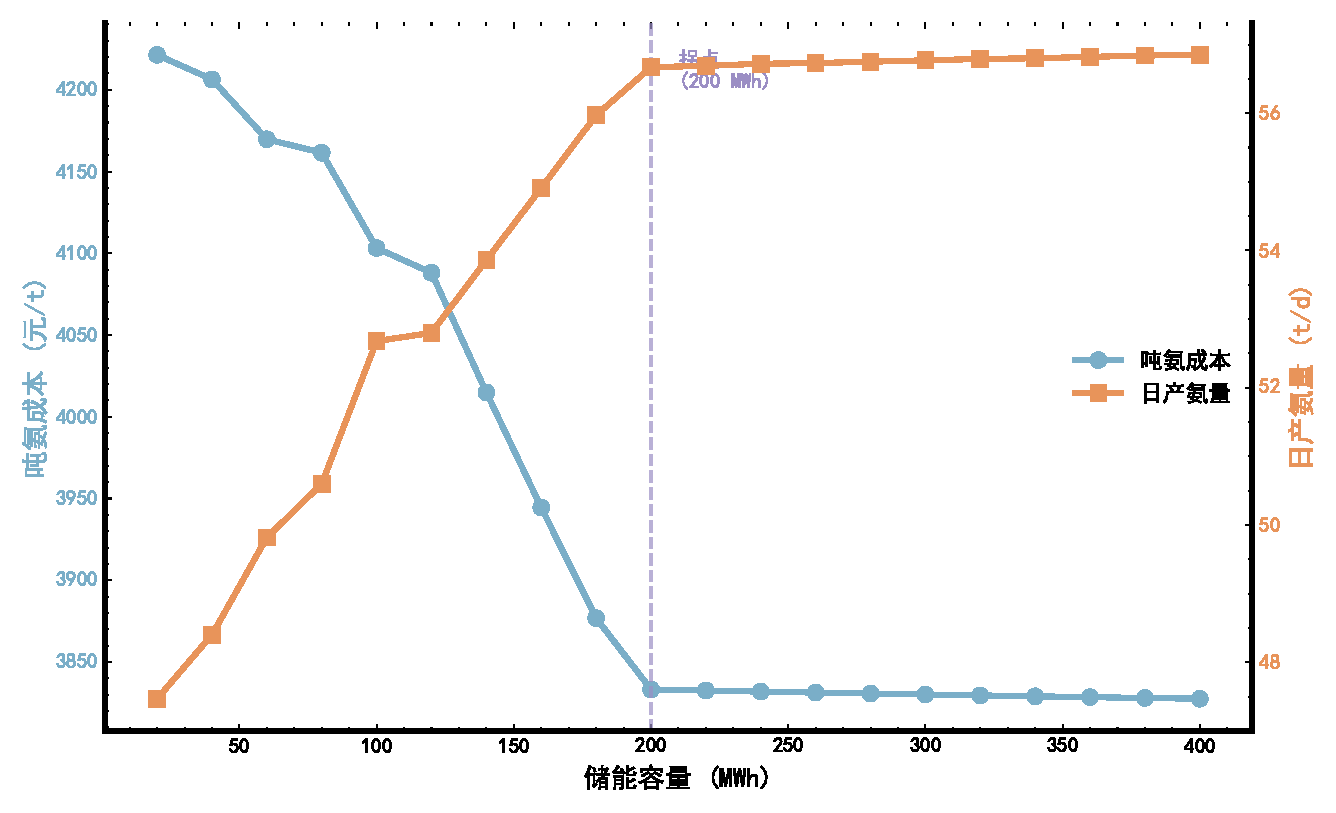
\includegraphics[width=0.82\textwidth]{figures/fig_q4_storage_optimization.pdf}
\caption{储能容量与吨氨成本、日产氨量关系曲线}
\label{fig:q4_storage_optimization}
\end{figure}

\begin{figure}[H]
\centering
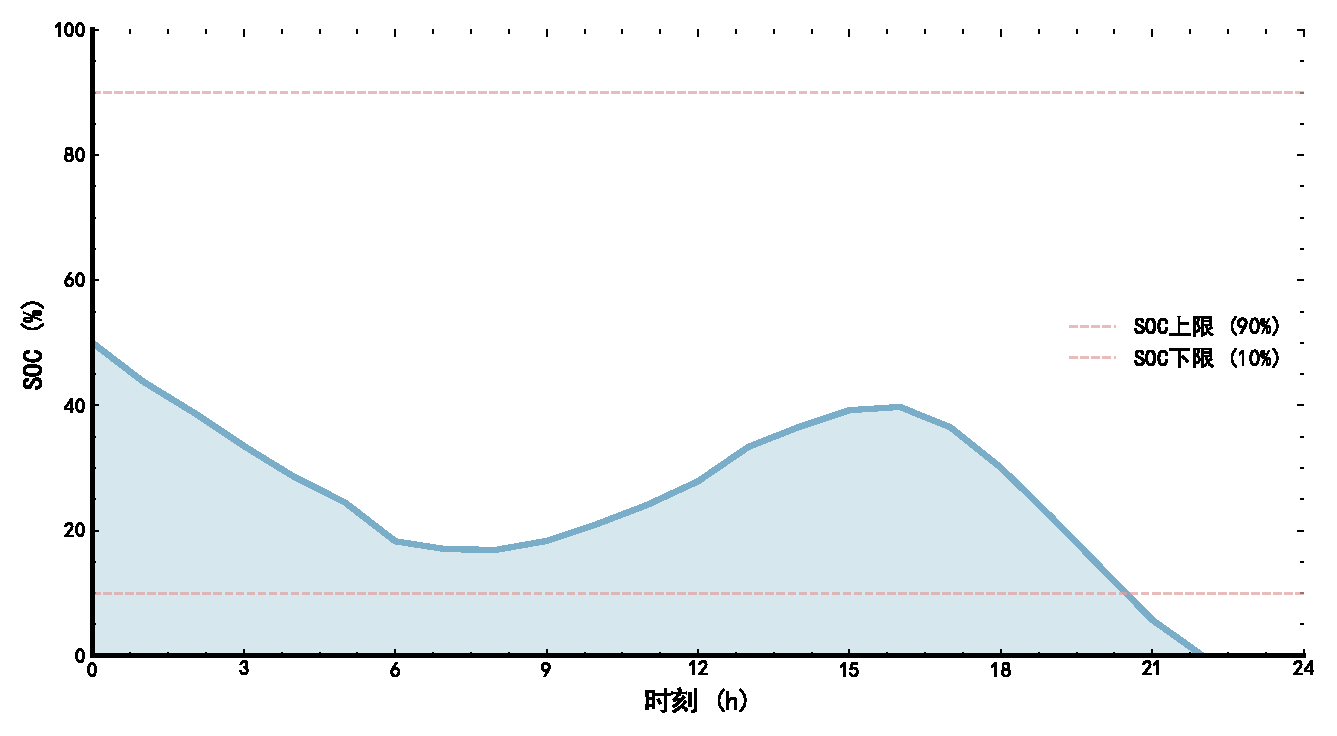
\includegraphics[width=0.82\textwidth]{figures/fig_q4_soc_curve.pdf}
\caption{最大弃电场景储能SOC变化曲线}
\label{fig:q4_soc_curve}
\end{figure}

\begin{figure}[H]
\centering
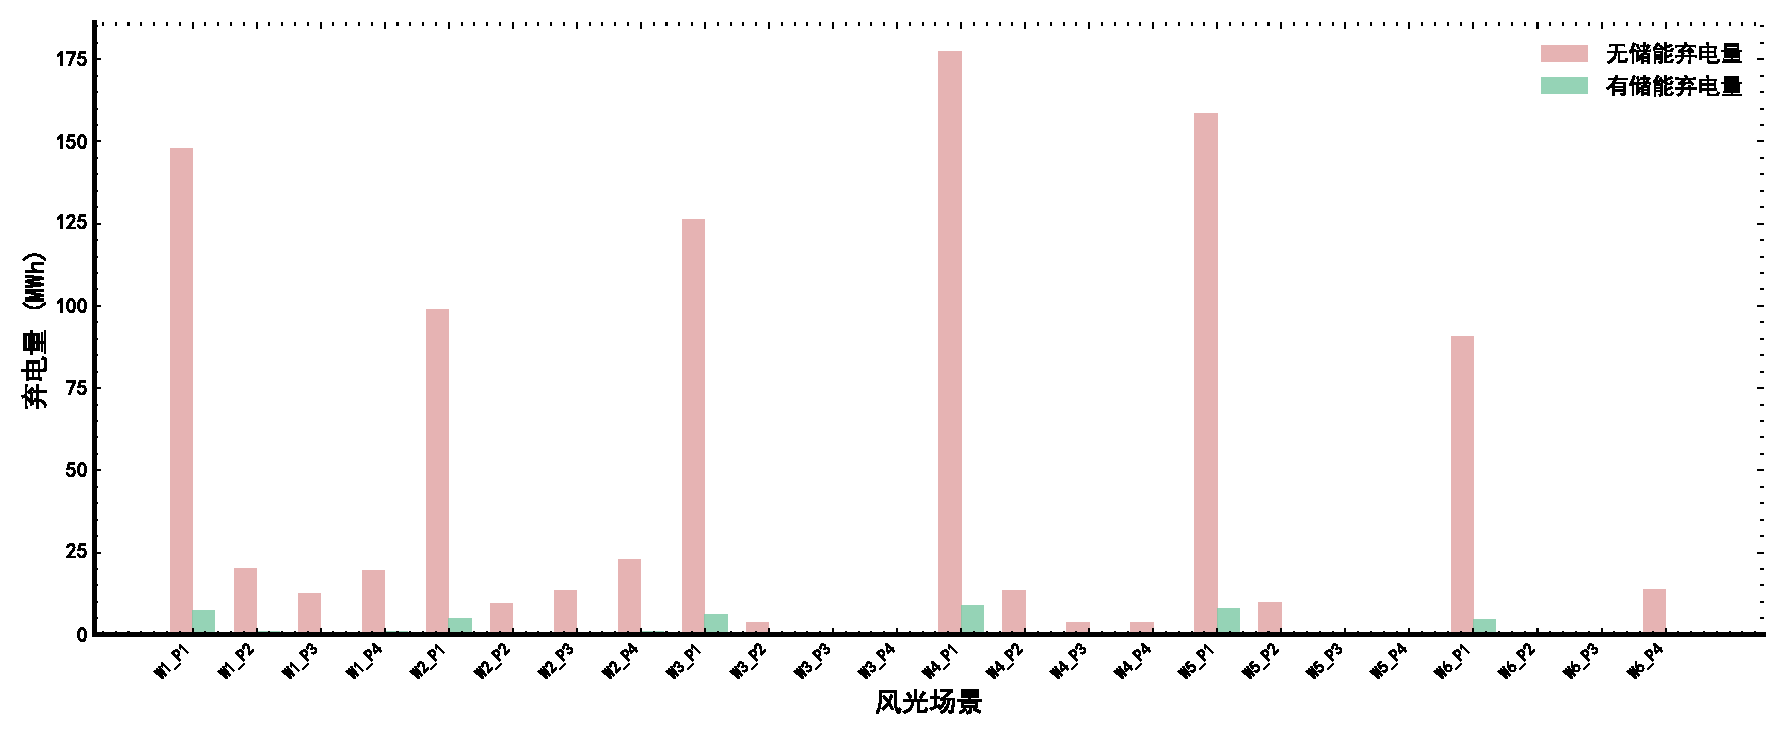
\includegraphics[width=0.95\textwidth]{figures/fig_q4_curtail_compare.pdf}
\caption{有无储能弃电量对比}
\label{fig:q4_curtail_compare}
\end{figure}

\begin{figure}[H]
\centering
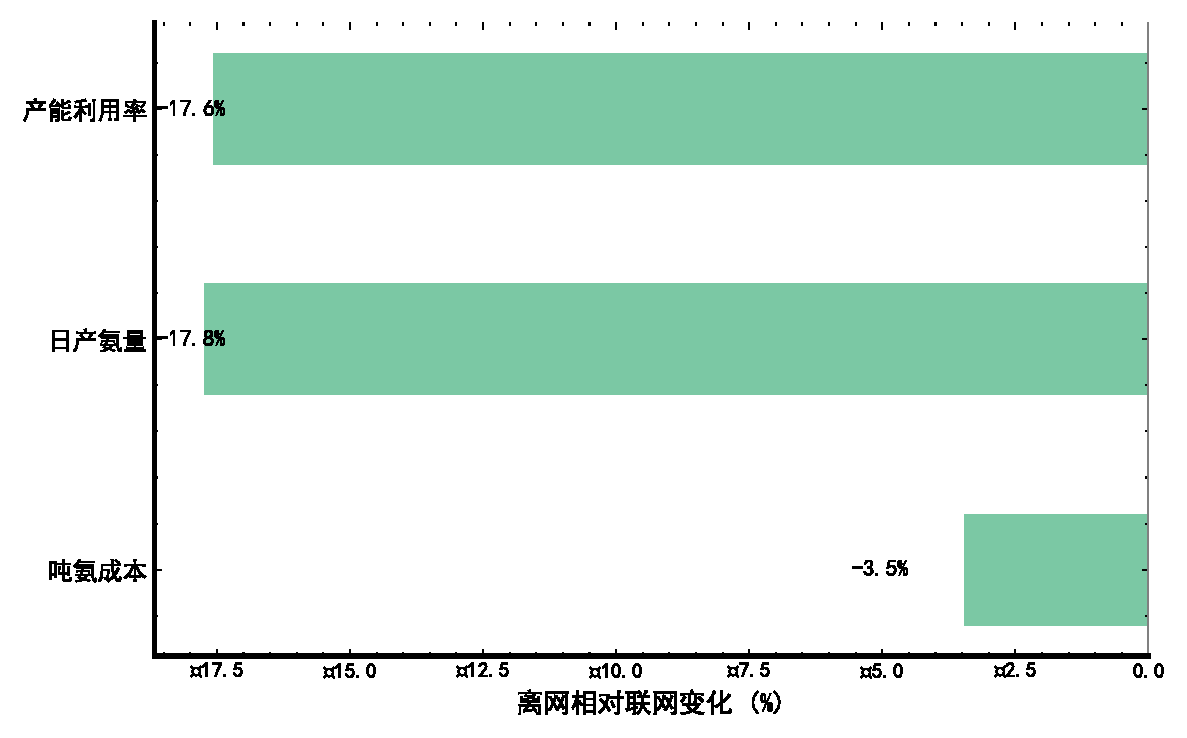
\includegraphics[width=0.75\textwidth]{figures/fig_q4_onoff_compare.pdf}
\caption{离网与联网运行模式经济性对比（发散柱状图）}
\label{fig:q4_onoff_compare}
\end{figure}

% ==================== 灵敏度分析 ====================

\begin{figure}[H]
\centering
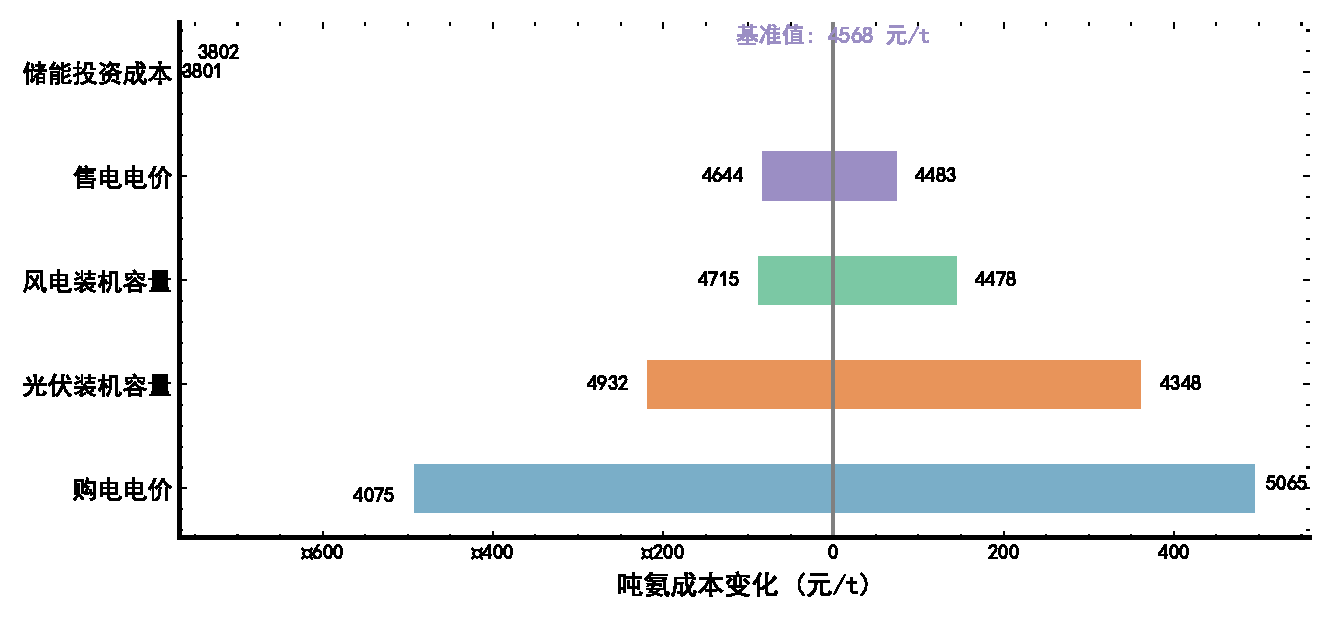
\includegraphics[width=0.82\textwidth]{figures/fig_sensitivity.pdf}
\caption{关键参数敏感性分析龙卷风图}
\label{fig:sensitivity}
\end{figure}
